% INSTRUCTIONS
% (1) Compile using LuaLatex (it is the successor of pdflatex). To check this on Overleaf, click on the Menu on the top left.
% (2) Complete the SETUP below

%%%%%%%%%%%%%%%%%%%%%%%%%%%%%%%%%%%%%%%
% DO NOT MODIFY FROM HERE ...
\documentclass[12pt,twosided]{ic_eee_thesis}


%... TO HERE
%%%%%%%%%%%%%%%%%%%%%%%%%%%%%%%%%%%%%%
% ADDITIONAL PACKAGES
% You can add your packages below. Note that the following packages are already loaded: pgfcore, geometry, bookmark, graphicx, setspace, kantlipsum, fontspec, polygrossia (default English), minitoc, silence, background, xpatch, tikzpagenodes, totcount, fancyhdr, titlesec and the tikz libraries calc, shapes.symbols and shapes.misc  

\usepackage[match]{luatexja-fontspec}
\setmainjfont{TakaoMincho}
\setsansjfont{TakaoGothic}
\bibliographystyle{ieeetr} %elsiver
\usepackage[figurename=Fig.,labelfont=bf,labelsep=period]{caption}
\usepackage{subcaption}
\usepackage{amsmath}
\usepackage{amsfonts} 
\usepackage{lmodern}
\usepackage{notoccite}


\hypersetup{
  colorlinks=true, % black,violet
  linkcolor=violet,  % 设置内部链接颜色 blue,teal
  citecolor=magenta, % 设置引用链接颜色 purple
  urlcolor=red     % 设置URL链接颜色 red
}



%%%%%%%%%%%%%%%%%%%%%%%%%%%%%%%%%%%%%%%
%%%%%%%%%%%%%%%%%%%%%%%%%%%%%%%%%%%%%%%
%%%%%%%%%%%%%%%% SETUP %%%%%%%%%%%%%%%%
%%%%%%%%%%%%%%%%%%%%%%%%%%%%%%%%%%%%%%%
% EDIT THE FOLLOWING INFORMATION WITH YOUR DATA
\title{Limit State Design Of Hybrid Joint With Slip-critical bolted joint and Bearing-type joint}
\subtitle{(摩擦と支圧を併用したハイブリッド継手の限界状態設計法に関する研究)} % use \subtitle{} to remove it
\author{Chen Yu}

\supervisor{Prof.Dr Takashi Yamaguchi \\[1mm] Prof. x Kitou} %UK: Dr no dot, prof has dot
\submityear{2024}
% PICK A DEGREE FROM THE LIST BELOW 
% DO NOT MODIFY THE NAMES
\course{Engineering}

\setboolean{list_of_figures}{true} % false or true 
\setboolean{list_of_tables}{false} % false or true 
\setboolean{acknowledgement}{true} % false or true 
\setboolean{acronyms}{true} % false or true - 

%%%%%%%%%%%%% END SETUP %%%%%%%%%%%%%%%
%%%%%%%%%%%%%%%%%%%%%%%%%%%%%%%%%%%%%%%

% ADDITIONAL COMMANDS
%Examples
\DeclareMathOperator{\diag}{diag}
\DeclareMathOperator{\vect}{vec}
%...


\begin{document}

\preamble % Do not change - required

% EDIT THE CONTENT OF THE FILES
% Abstract.tex
% OrigSta_Copyright.tex
% Acknowledgement.tex
% You can find them under the folder 
% "chapters" on the left column

% ADD AS MANY CHAPTERS AS NEEDED
% BY CREATING .TEX FILES IN THE FOLDER chapters
% AND ADDING \input{namechapter.tex} BELOW

\chapter{Introduction}
\label{ch1}

%%%%%%%%%%%%%%%%%%%%%%%%%%%%%%%%%%%%%%%
% IMPORTANT
\begin{spacing}{1.25} %THESE FOUR
\minitoc % LINES MUST APPEAR IN
\end{spacing} % EVERY
\onehalfspacing % CHAPTER
% COPY THEM IN ANY NEW CHAPTER
%%%%%%%%%%%%%%%%%%%%%%%%%%%%%%%%%%%%%%%

\section{Background}

Since the 18th century, iron, steel, and concrete have replaced timber and stone in the design, manufacture, and construction of large modern structures, including bridges. In the case of steel structures, components are factory-manufactured and then delivered to the construction site, where they are assembled or connected on site. Units are transported in members that are manufactured in factories. The members consist mostly of steel plates, and the main objective is to connect them together through a process called 'splicing'.

Steel bridges constructed between 1860 and 1955 were predominantly connected with riveted joints \cite{Quentin2012MorphogenesisStructures, COLLETTE2014, Ambroziak2023CASEANALYSIS, Collette2012Les18401940, Costa2013RehabilitationBridge}, as shown in Fig.\ref{fig-intro1} (Photo by Luca Upper \cite{lucaphoto}). In Japan, the period of cast iron started in 1897 which later shifted towards steel industry. The joints were riveted until the introduction of welding in the 1950s, where 40 kg grade SS39A and SS41 structural steel were used \cite{rivet1934}. This ancient type of joint allows secure connection of two or more metal sheets. Rivets are placed in the hole, then heated to high temperature by a pneumatic hammer which forms a head. After it cools down, a residual clamping force is created, making a riveted joint possible.

\begin{figure}[htbp]
    \centering
    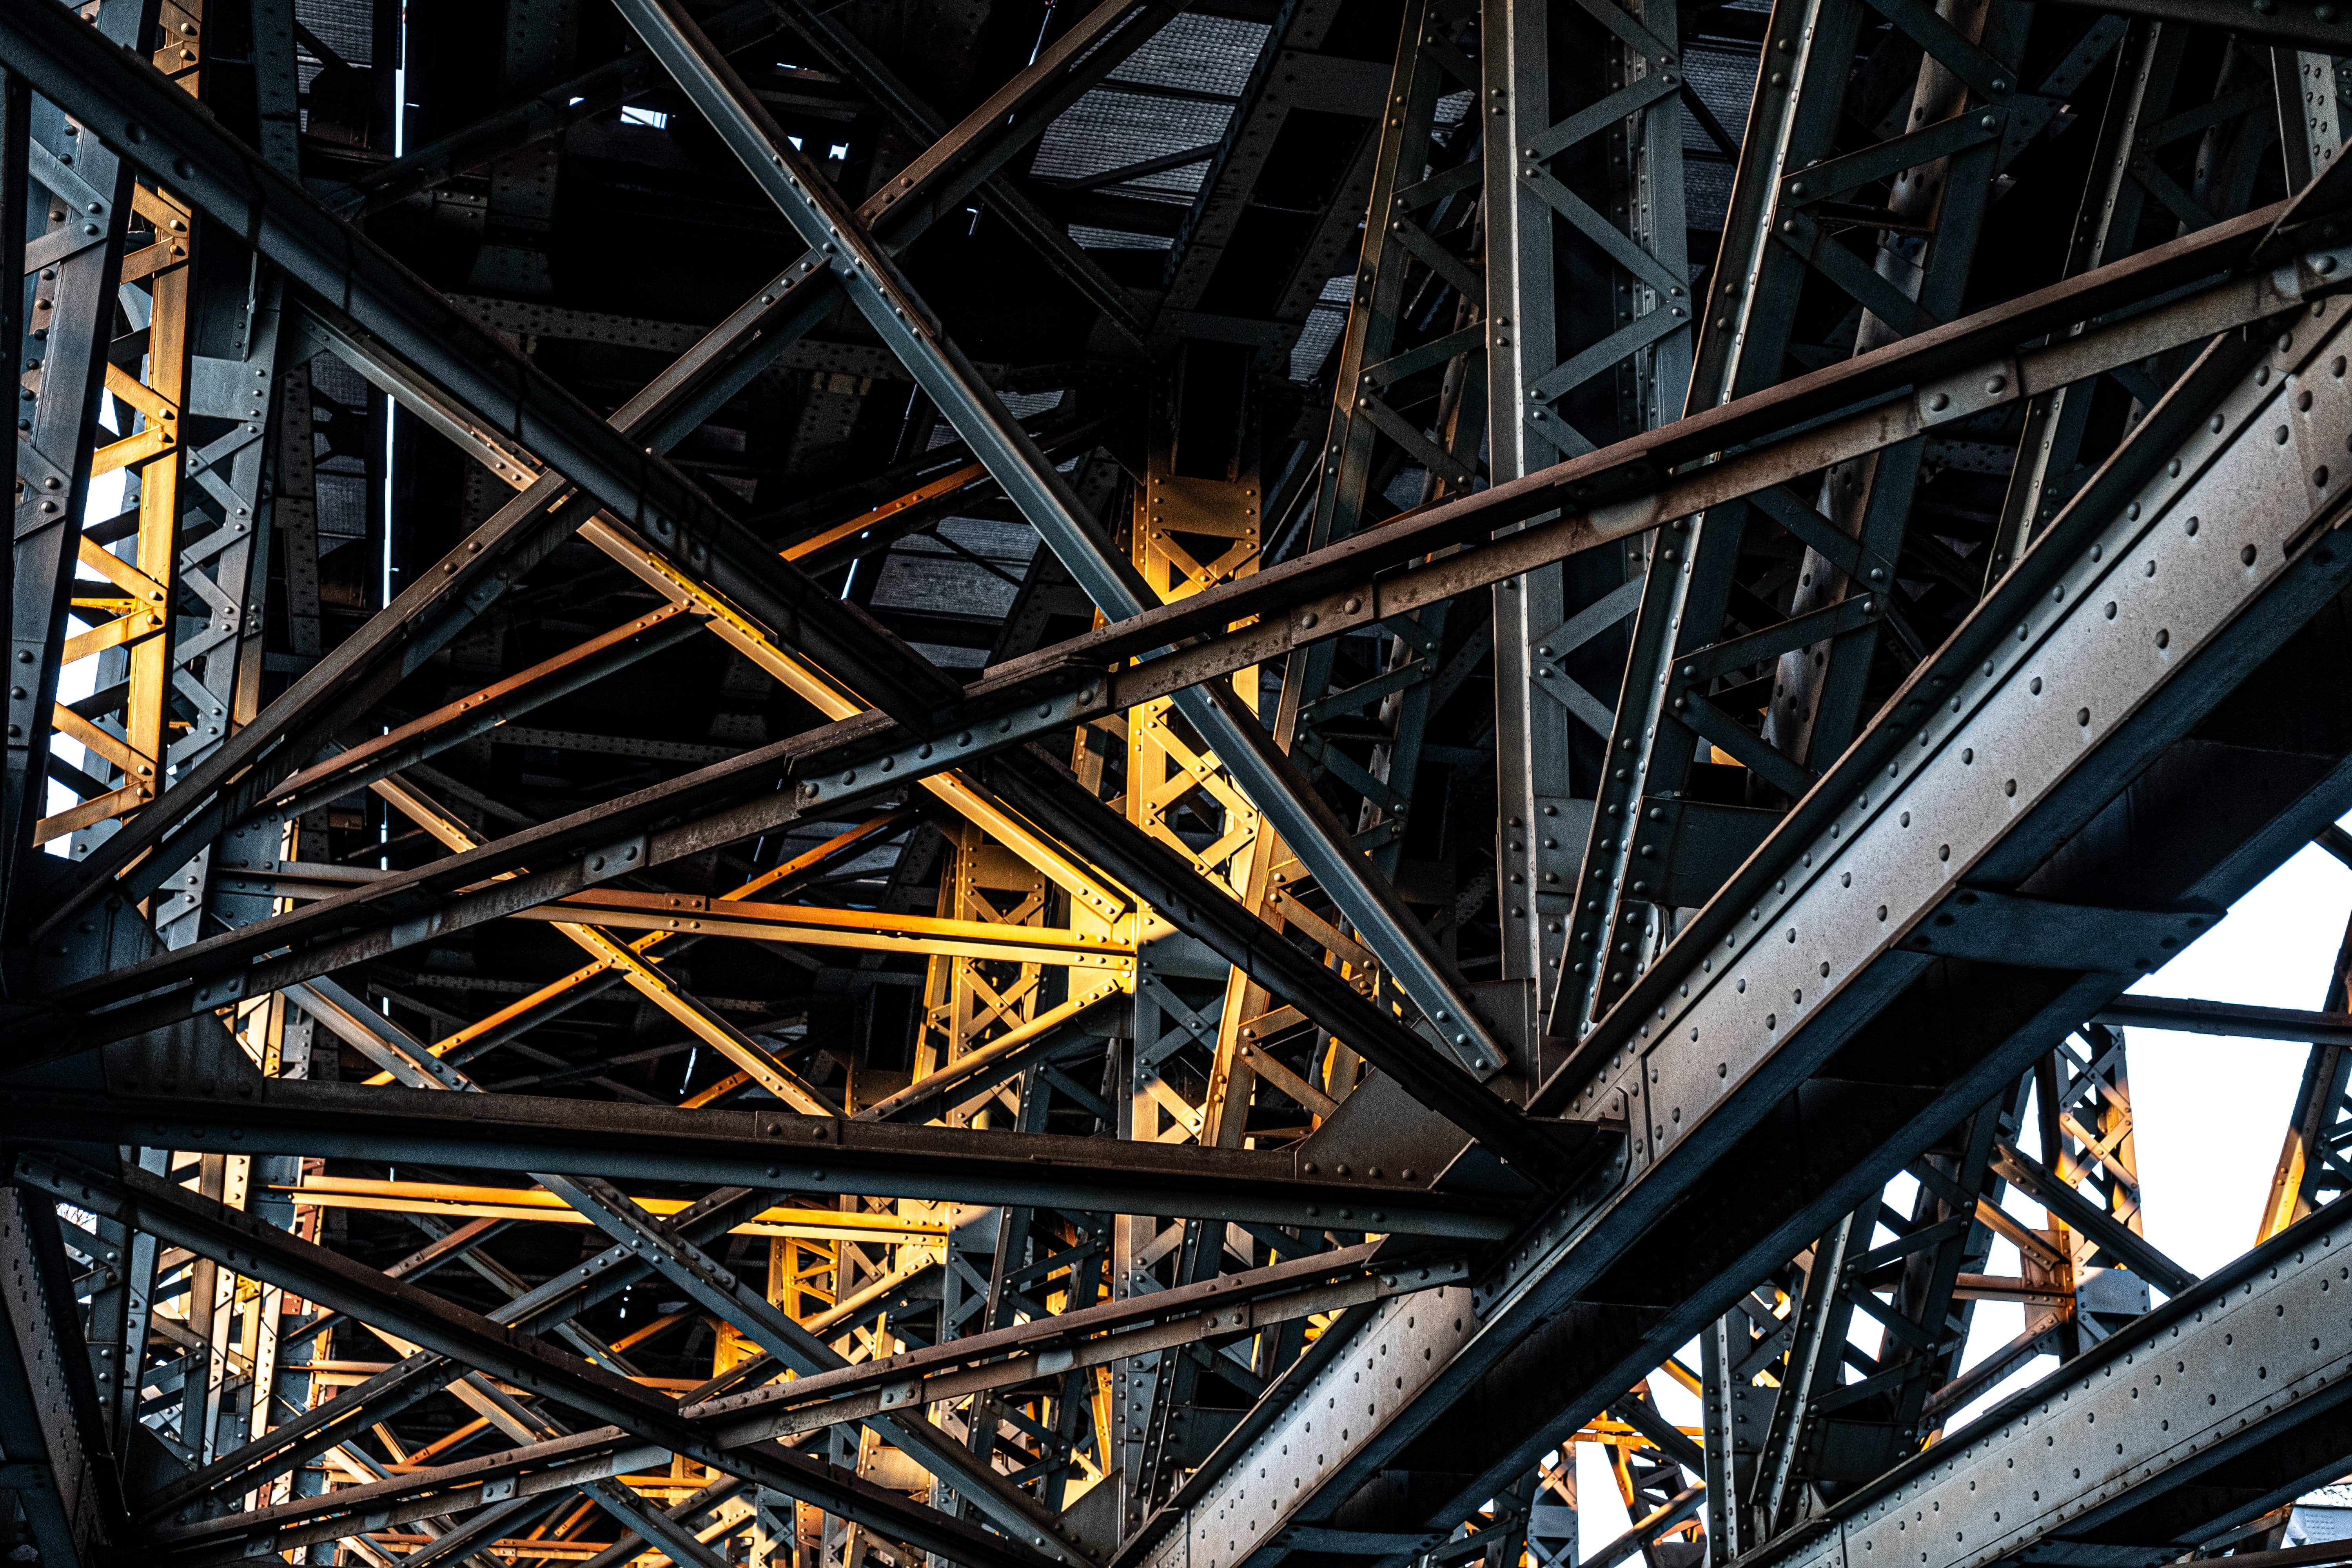
\includegraphics[width=0.85\textwidth]{imgs/intro/steel-structure.jpg}
    \caption{Riveted joint of railway bridge in Switzerland (Photo by Luca Upper)}
    \label{fig-intro1}
\end{figure}

After 1955, advancements in steel technology enabled the production of high-strength steel. As a result of the bolt's ease of construction and its reliable mechanical transmission mechanism, it quickly supplanted the rivet as the prevailing joining method.

\ac{HSB} have three types of connection: friction connection, bearing connection, and tension connection. Out of these, the friction connection is the most commonly used.

Friction type connections (also referred to as friction connections) involve joining materials that transmit stress through frictional resistance generated by the inter-material compressive force produced when the jointing materials are tightened using high-strength bolts. Stress is transferred via compressive forces between materials that are dispersed around the bolt, unlike in riveted joints where stress is transmitted through local bearing forces. This results in decreased stress concentration and smoother flow of stress. Another advantage is there is no misalignment between the joined materials until the application of a force which exceeds the frictional resistance can cause the friction to break and slip to occur, thus ensuring exceptionally high rigidity and fatigue strength.

Welding was first applied to steel bridges in the 1930s \cite{ALENCAR2019154}. And arc welding was first invented in the late 19th century, with high-density energies, like electron and laser beams, being applied to welding in the late 20th century. Welding conncetions are usually carried out in the factory due to the stringent construction conditions on site.

%todo!

%Insert 3 type of joint
Each of the three different types of connection has its own advantages and disadvantages, and no combination can completely replace any of them. And occasionally it is necessary to use two different types of joint at the same time, probably because of the lack of skilled labour (for repair riveted bridge, rivet combined with HSB), the inability of the joint surface to meet the required slip coefficients (Friction type combined with Bearing type connection) as well as the need to increase the strength of the joint to shorten the joint length (HSB combined with welded connection), etc.

%hybrid history


\begin{figure}
    \centering
    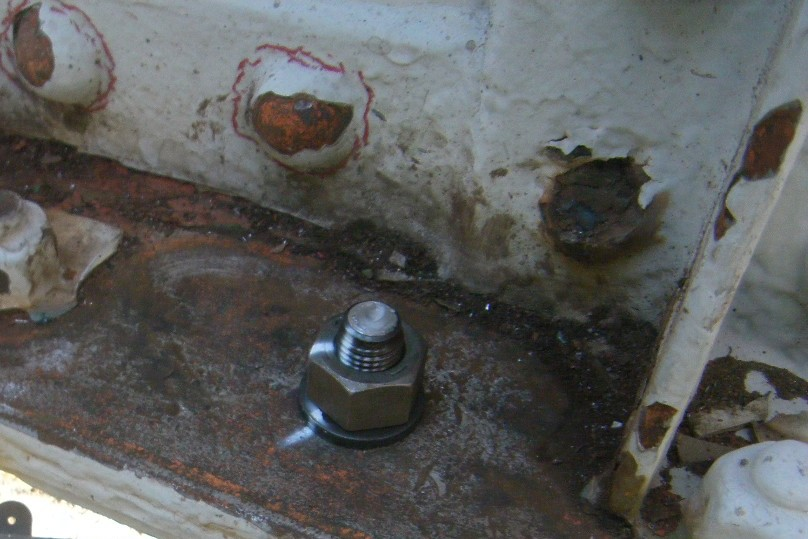
\includegraphics[width=0.8\textwidth]{imgs/intro/HSB-rivet.JPG}
    \caption{Rivet partially replaced by HSB of Hazukawa Riveted bridge in Fukui Japan}
    \label{fig-tprivet}
\end{figure}


\section{Technical Problem}

During the reconstruction projects following the Second World War, the combined use of diverse connection methods with varying principles presented challenges. For instance, when reinforcing aging riveted structures by welding or partially replacing them with \ac{HSB}, difficulties arose as shown in Fig. \ref{fig-tprivet}. Joining components with combined different load transfer mechanism connection methods results in a non-stationary structure, making it difficult to accurately calculate the sharing of loads in the past. As a result, only one of the two types was considered valid for design purposes at the time, ignoring the cooperative actions expected from their combined use.

The maintenance and repair of ageing bridges are expected to encounter growing obstacles in the near future. Bridges must achieve a compromise between suitable flexibility and rigidity. The addition of reinforcing elements to a completed bridge may upset this equilibrium and create problems. Consequently, post-construction reinforcement of a bridge may present a challenge by using hybrid connection.

In addition, for new structural components, the rational use of hybrid joints can effectively improve the strength of the joints and shorten the length of the joints as much as possible, while meeting the required strength to make the joint compact.  However, unlike the reinforcement of an existing structural component, new structural components raise issues of structural stability, durability and strict requirements for allowable deformation, and require a series of tests before they can be installed.

In summary, this work focuses on the following technical issues:

\begin{itemize}
    \item The primary technical challenge lies in the lack of understanding regarding the load transfer mechanism when combining connections with different mechanical principles.
    \item For the use of hybrid joints, not only to understand how the load is transmitted, but also to understand how the fasteners should be reasonably arranged. Different arrangements may produce different load transfer effects, so exploring the reasonable fastener arrangement scheme will be an important technical problem.
    \item The stiffness of Friction connection and bearing connection are different. In the case of a friction connection, there will be a small elastic dislocation (slip) before occurrence, which is a different mechanical mechanism from the elastic deformation of a bearing connection. Exploring the deformation capacity of the bearing and friction combination is also an important technical subject.
    \item After understanding the load transfer mechanism, strength and deformation performance of hybrid connections, it is necessary to define their limit states and to devise how to differentiate between the limit states and their corresponding strength equations.
    
\end{itemize}



\section{Aims and Scope}

This work is separated into two sections. The initial section entails repairing and enhancing aging riveted bridge through the replacement of damaged rivets with high-strength bolts using a friction connection. This technique is deployed to create hybrid joints that can jointly resist loads. The second section discusses the use of hybrid joints in the construction of new bridges. Such bridges encounter various design challenges, including the need to enhance component strength in response to increased external live loads without enlarging the structure size. These adjustments have become necessary in recent years, coinciding with the emergence and use of high-strength steels. The joints should be designed to withstand the increased strength of the steel components. However, the strength of friction joints is dependent on the number of bolts and slip coefficient. Enhancing the slip coefficient can effectively increase the joint strength, but this is an uncontrollable factor with significant construction costs. Therefore, it is imperative to suggest a cost-effective means of enhancing joint strength in high-strength steel structures without enlarging the joint size.
%本工作大体分为两个部分,第一个部分为(现存)老旧铆钉桥接头的补修补强,通过用高强螺栓替换部分已经损坏的铆钉以达到混合接头共同抵抗载荷的作用。第二部分为新建桥梁混合连接的应用,新建桥梁会面临很多设计合理性的问题,比如在外部活荷载日益增多的情况下如何在不增大桥梁结构的同时增强其部件的强度是近几年需要面临的调整,伴随着高强度钢的出现与应用,其接头也应当随着钢部件强度的上升而提高,然而摩擦接合的强度取决于螺栓的数量和滑移系数,滑移系数的提高能有效增强接头的强度,然而滑移系数是不可控且施工成本很高。因此需要提出一种低廉的可以增强接头强度的接合方法来应对高强度钢结构。

Investigating the riveted joint contact surfaces of aging riveted bridges is necessary to provide a reliable slip coefficient for the friction connection, which is essential in calculating the strength of hybrid joints consisting of rivets and high-strength bolts in existing steel structures. This is because high-strength bolt friction connections resist loads through friction at the interface. When replacing the rivets, it is important to take special care during removal as the rivets may still be sharing part of the load, particularly in areas where there is more load sharing. It must be ensured that the load originally resisted by the rivets is appropriately transferred to other rivets to avoid potential damage to neighbouring rivets. Hence, an examination of the method by which the load is distributed within riveted joints, both with and without a specific damaged rivet, and replacing it with high-strength bolts is essential. The removal of a rivet affects the mechanism of load redistribution, necessitating careful consideration in the bolt arrangement to ensure that high-strength bolts can aptly withstand external forces.  Once the principle of redistributing the load after removing individual rivets is understood, it becomes necessary to systematically arrange high-strength bolts and explore the load transfer mechanism of the hybrid joint. The high-strength bolts exhibit high stiffness and distinct deformation performance from riveted joints, necessitating an investigation into the deformation performance of the Rivet-HSB hybrid connection. Also, it is essential to investigate the load-carrying capacity of hybrid connections and establish a limit state in accordance with the allowable deformation value.

For hybrid connections composed of a combination of rivets and high-strength bolts, this study concentrates on achieving the following aims:

\begin{enumerate}
    \item Provide reliable slip coefficients for riveted connections
    \item Investigate the mechanism of load redistribution after removing individual rivets
    \item Investigate the load transfer mechanism and deformation performance of hybrid rivet-\ac{HSB} connections
    \item Differentiation of limit states and proposal of strength calculation formulas
\end{enumerate}
%首先是对于现存钢结构的铆钉和高强螺栓的混合接头,由于高强螺栓摩擦接头是通过界面的摩擦来抵抗载荷的,因此调查老旧铆钉桥的接合面是有必要的,需要为摩擦结合提供一个可靠的滑移系数以计算接头的强度。然后再更换铆钉时,由于铆钉可能仍然分担着一部分力,特别是对于载荷分担比较多的区域,在拆除铆钉时需要特别注意原本铆钉抵抗的这部分力会转移到其他铆钉上,这有可能会造成相邻铆钉发生损坏,因此,在用高强螺栓部分更换铆钉时有必要调查清楚铆钉接头的载荷分担方式以及拆除某一个铆钉时,载荷会如何进行再分配,从而可以更好的进行配置高强螺栓,使得高强螺栓能合理的承载尽可能多的外力。了解了拆除个别铆钉后才分配原理之后,就需要合理的进行安排高强螺栓,并探讨结合了高强螺栓的混合接头的力学传递机理以及其变形能力,由于组合了刚度较高的高强螺栓,因此其变形能力和铆钉接头会有所区别,探讨其承载能力以及根据形变量来定义一个极限状态是必须的。
%对于铆钉和高强螺栓组合成的混合接头,本工作着重解决以下几个目标:
%1. 铆钉接合面的滑移系数
%2. 拆除铆钉时,铆接的再分配原理
%3. 铆钉-高强螺栓混合接头的力学传递机理及其变形能力
%4. 极限状态的区分以及强度计算式的提案

Secondly, for newly constructed steel bridges, bearing-type connections as substitutes for rivets have emerged as interference-fit bolts. In recent years, research on injection bolts and high-strength mechanical rivets has also progressed. This work focuses on the discussion of interference-fit bolts as bearing-type connections and a combination of high-strength bolt friction connections. The development and proposal of such hybrid connections were the main research objectives of this work. The feasibility of the hybrid connection will be explored first through numerical analysis, where, although the mechanical transmission mechanism is unknown, the approximate joint strength can still be obtained through simple accumulation of each fastener (unlike the hybrid connection of welding and high-strength bolts, the connection strength cannot be calculated by accumulation, which will be explained in detail in Section \ref{sec-hsbweld}). Secondly, if pretension is applied to the interference fit bolts,the bolts are tightened, and the tensioned part of the shaft may produce small gaps with the bolt hole wall. The mechanism by which pretension affects the bearing resistance of the interference fit bolts needs to be explored. Similar to the hybrid connection between rivets and high-strength bolts, the deformation capability of IFB and HSB hybrid joints also needs to be discussed. Owing to the higher pretension applied to the IFB and its different material properties compared to rivets, the deformation performance may vary. The purpose of this work is to explore the deformation performance of the connection, define its ultimate state, and propose a strength calculation equation based on theoretical, experimental, and analytical results.

%其次是对于新建钢结构来说,承压型接作为铆钉的替代过盈配合螺栓最早出现,近几年注射螺栓以及机械式高强铆钉的研究也出现了进展,本工作着重探讨过盈配合螺栓作为承压型连接和高强螺栓摩擦连接组合成混合连接,发展并提案此类混合连接是本工作的重点研究,研究首先会通过数值解析探讨混合连接的可行性,尽管不知道力学传递机理,但是依然可以通过简单的承载力累加得出大概的接头强度(这与焊接和高强螺栓的混合连接不同,后者无法通过累加的方式来计算获得接头的强度,在之后的章节\ref{sec-hsbweld}会进行详细的解释)。其次如果对过盈配合螺栓如果施加预紧力,螺栓则会产生紧缩效应,轴部紧缩后的螺栓可能会与螺栓孔壁产生微小的缝隙,预紧力是否会影响过瘾配合螺栓承压抵抗的机理有待探讨。和铆钉-高强螺栓混合接头一样,IFB和HSB的混合接头一样需要讨论其接头的形变能力,由于IFB会施加较高的预紧力,且其材料特性和铆钉不太一样,因此形变能力也会有所差别,探讨接头的变形能力,定义其极限状态,并通过理论,实验,解析结果分析并提案一个强度计算式是本工作的目的。

%对于IFB和HSB组合的混合接头,本工作着重解决以下几个目标:
%1. 混合接头的可行性研究
%2. IFB施加预紧力给承压连接带来的影响
%3. 探讨IFB-HSB混合接头的力学传递机理,及其形变能力,并给出最合适的螺栓配置方案。
%4. 极限状态的区分以及强度计算式的提案

%最后需要总结两种不同的承压连接和摩擦连接的混合接头,并总结分析提出一个混合接头的极限状态设计法是本工作的最终目标。

For the hybrid connection of IFB and HSB, this work focuses on the following objectives: 

\begin{enumerate}
    \item Feasibility study of the hybrid connection. 
    \item Investigation of the effects of preload for IFB on bearing-type connections.
    \item Exploration of the load transmission mechanism and deformation performance of the IFB-HSB hybrid connection, and provision of the most suitable bolt arrangement plan.
    \item Differentiation of the limit state and proposal of a strength calculation formula.
\end{enumerate}

Lastly, it is necessary to summarize and analyze the hybrid connections of the two different bearing-type connections and friction-type connections, and to propose a design method for the limit state of the hybrid connection and the strength calculation formula. This is the ultimate goal of this work.





\section{Research Approach And Thesis Outline}

Firstly, the theoretical background on bearing-type and friction-type connections will be reviewed, followed by an exploration of installation methods and material properties of fasteners.

Based on this literature review, a preliminary selection will be made on the important parameters in the choice of alternative products to be further investigated, such as the type of fastener. Then, taking the information from literature as a basis, the conditions required for hybrid joints are explored in detail and a computational model is proposed to evaluate the method for strength calculation as well as the mechanical distribution mechanism of hybrid joints.

The main body of this research project is based on the fundamental approach of numerical analysis and experiment. Conduct a finite element analysis project to investigate the load transmission mechanism using Abaqus analysis software. Test hybrid joints with partially replaced HSB under riveted joints and hybrid joints with high strength bolts combined with IF bolts to validate the analysis results. This will be performed by testing double lap shear connections with Rivet \& \ac{HSB} or \ac{IFB} \& HSB in the Osaka Metropolitan University Mechanical Laboratory.

Finally, the results obtained from the double lap shear tests and analysis are processed to gain the load transfer mechanism, hybrid joint strength and the condition of limit state.

Lastly, the test results obtained will be used to propose a limit state design method for the hybrid joint combined bearing and friction type connection.

The study's purpose was broadly categorised into three objectives: 1) Clarify the Mechanics Behaviour of Bearing and Friction Hybrid Joint, 2) Define the limit state for the hybrid joint, and 3) Propose design methods and strength equations. An overview of the steps taken in this research project is shown in the diagram on the following page as shown Fig. \ref{fig-rflow}.

%research flow
\begin{figure}
    \centering
    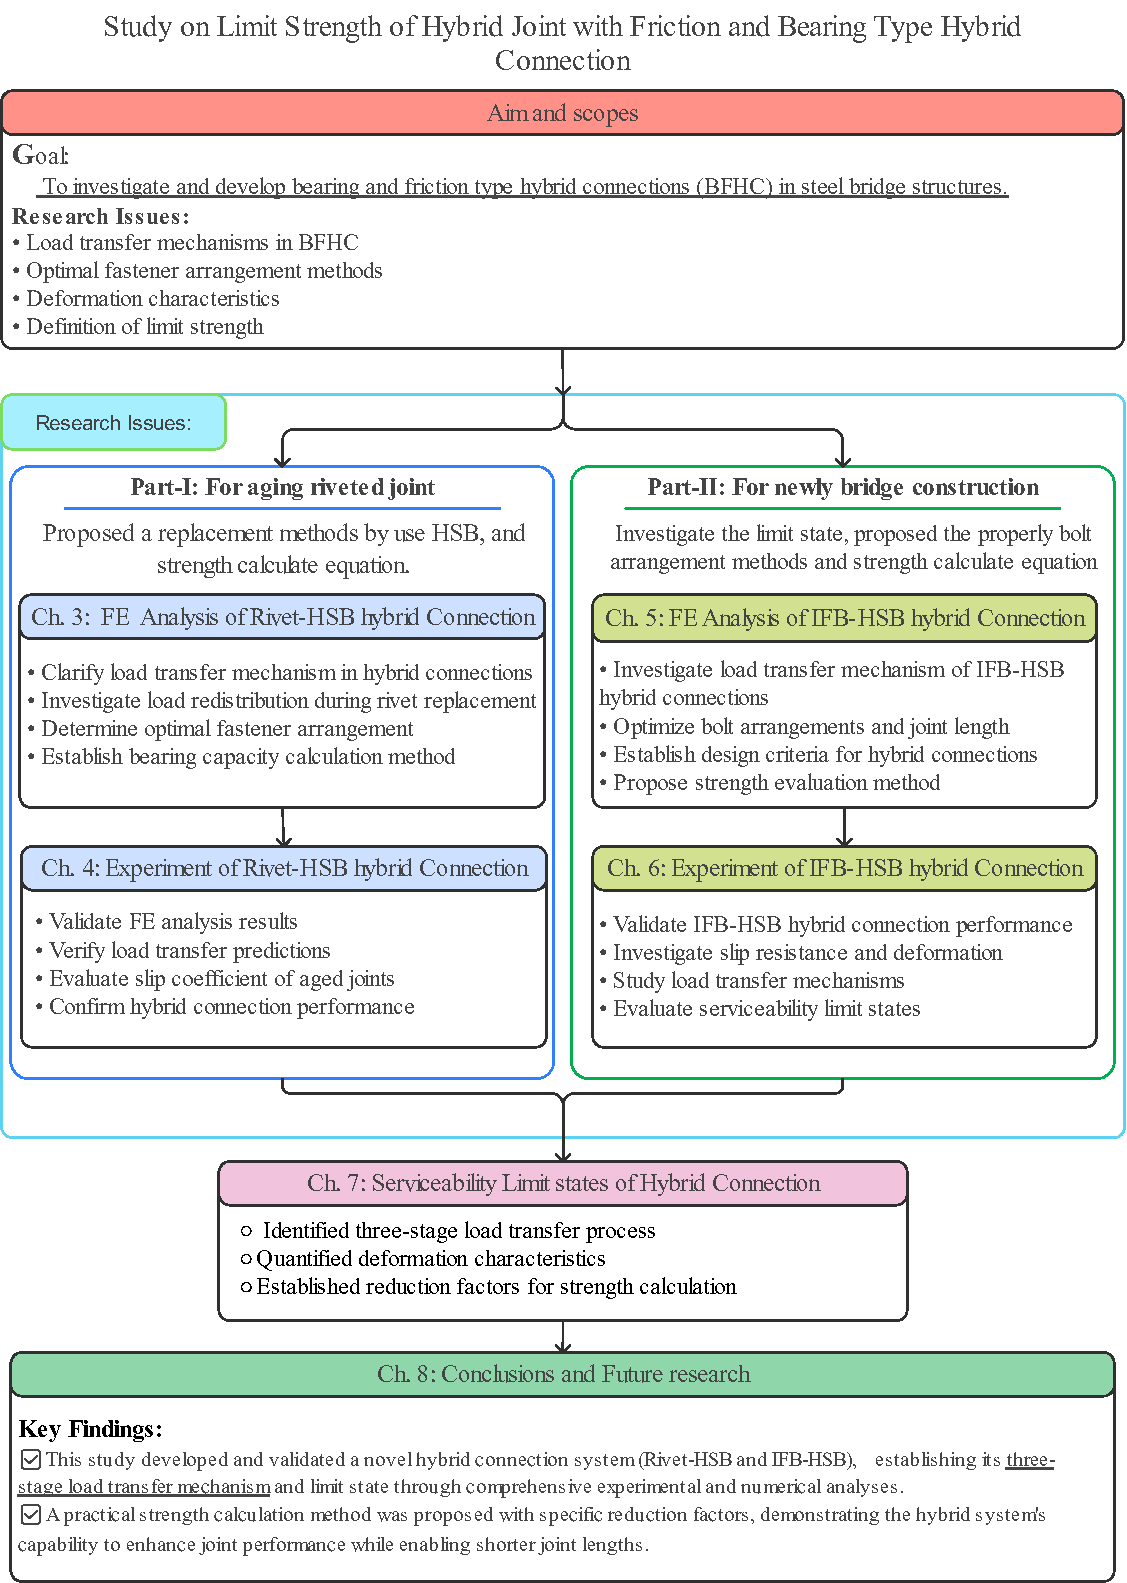
\includegraphics[width=\textwidth]{imgs/intro/research-flow.pdf}
    \caption{Overview of work flow of this research project}
    \label{fig-rflow}
\end{figure}
\chapter{State of the Art}
\label{ch2}

%%%%%%%%%%%%%%%%%%%%%%%%%%%%%%%%%%%%%%%
% IMPORTANT
\begin{spacing}{1.25} %THESE FOUR
\minitoc % LINES MUST APPEAR IN
\end{spacing} % EVERY
\onehalfspacing % CHAPTER
% COPY THEM IN ANY NEW CHAPTER
%%%%%%%%%%%%%%%%%%%%%%%%%%%%%%%%%%%%%%%

\section{Riveted connection}

Before the development of welding technology and \ac{HSB}, rivets were commonly used to join steel structures. In particular, steel bridges built between 1860 and 1950 were almost exclusively riveted. In Japan, the era of cast iron began in 1897 and gave way to the era of steel. Until the introduction of welding in the 1950, riveted joints were used with 40 kg class structural steel (SS39A, SS41)\cite{rivet1934}. This oldest type of joint allows two or more metal sheets to be joined together. After being heated to a high temperature, the rivets are placed in the hole and a pneumatic hammer is used to form the other head. The rivet is then cooled to create a residual clamping force, thus realising the riveted joint.

However, riveting requires skilled techniques and has problems and hazards such as noise and fire, so it is rarely used for new structures and is no longer described in the Road and Bridge Specifications after 1980. Welding, on the other hand, became the main method of fabricating members in factories around 1955 due to advances in welding technology and economic efficiency. Rivets also ceased to be used on site around 1965 due to a reduction in the number of riveters and noise problems, and were replaced by high-strength bolts.

Steel riveted bridges have significant cultural and historical value as part of our constructive heritage from the previous century. Numerous iron and steel riveted bridges are of historical importance, requiring restoration and preservation, and ongoing use. A large number of riveted bridges have been rebuilt due to age and corrosion, but many riveted bridges are still in service \cite{COLLETTE2014}. Most of the riveted bridges that remain today are more than 60 years old from the time of construction and, although it depends on the maintenance method, some age-related deterioration has been reported, including corrosion as shown in Fig.\ref{fig-corriv} where almost all rivet heads have disappeared, fatigue cracking and rivet loosening as shown in Fig.\ref{fig-losriv} and Fig. \ref{fig-rivetisu}.

\begin{figure}[htbp]
    \centering
    \begin{subfigure}[t]{0.85\linewidth}
        \centering
        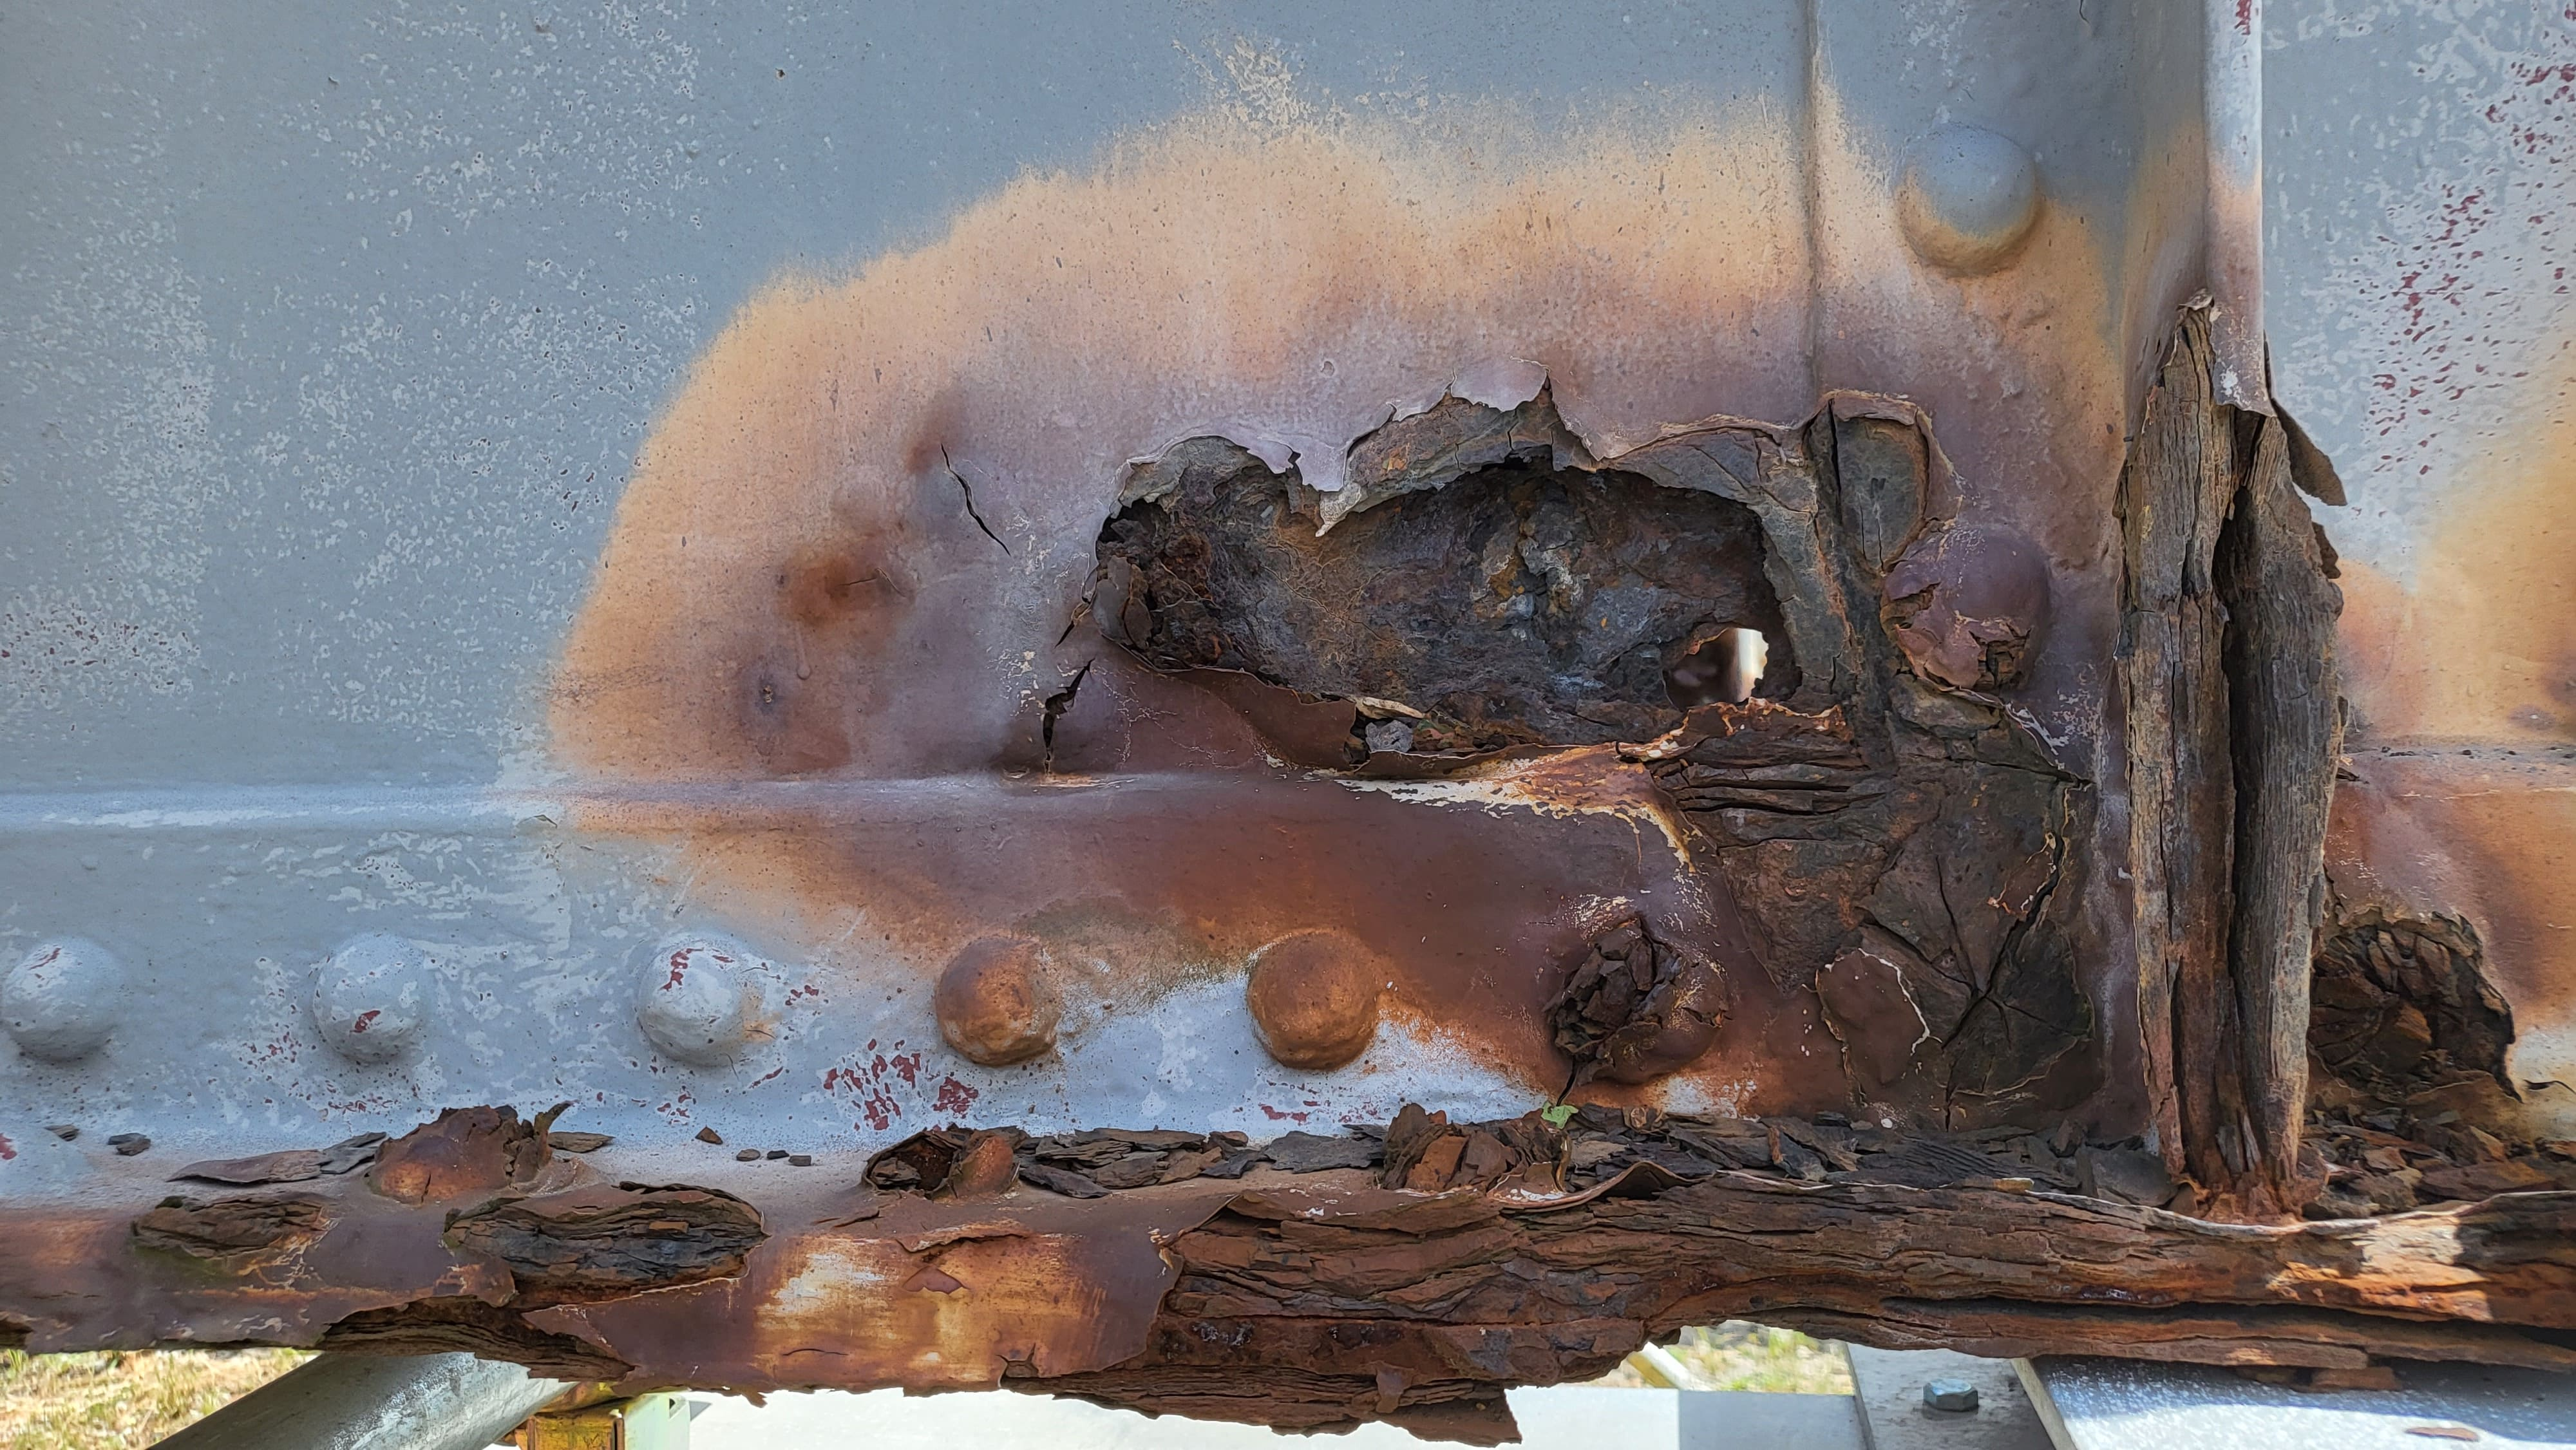
\includegraphics[width=\textwidth]{imgs/ch2/rivet-cor-1.jpg}%rivet-cor.png
        \caption{Corrosion of rivet}
        \label{fig-corriv}
    \end{subfigure}
    
    \begin{subfigure}[t]{0.85\linewidth}
        \centering
        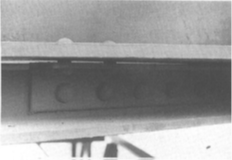
\includegraphics[width=\textwidth]{imgs/ch2/rivet-loss.png}
        \caption{Loosing of rivet \cite{rivet1977}}
        \label{fig-losriv}
    \end{subfigure}
    \caption{Aging condition of rivet}
\end{figure}


\begin{figure}[htbp]
    \centering
    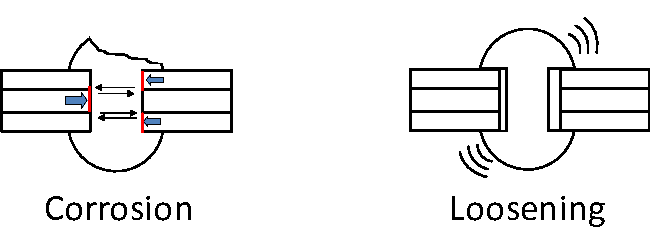
\includegraphics[width=0.8\textwidth]{imgs/ch2/rivet-issue.pdf}
    \caption{corrosion and loosing of aging rivet}
    \label{fig-rivetisu}
\end{figure}

\subsection{Mechanical behavior of riveted joint}

There are three types of resistance present in a riveted joint: friction, bearing, and shear. When it comes to force transfer utilizing a single rivet, there are two types: single-lap and double-lap as shown in Fig.\ref{fig-lapconnec}. Although an increase in the number of plates results in multi-sided shear, these two types are the fundamental structures of riveted joints in terms of force action. The forces transferred by the rivet only take into account the forces perpendicular to the rivet axis, such as direct tensile force. They do not consider the impact of axial tensile forces on the rivet head or its design. When two plates are joined by riveting, frictional forces transmit the load and restrict plate movement. This enhances the joint's strength, although it is not considered during the design process. Fig.\ref{fig-rsdisri} illustrates that the stress distribution, encompassing the rivet and the plate, is highly intricate. However, for practical purposes, it can be simplified into the following three types to facilitate design calculation for engineering.

\subsection{Design methods}

Riveted joints can be classified into approximately five types of failure model, depending on the strength of the rivet and the strength of the steel. Fig. \ref{fig-beafalmode} shows a fracture image of a single shear rivet. However, since the fracture of the main plate can be prevented by considering the placement of the rivets (model c--e), the shear strength of the rivets and the bearing strength are considered, and the strength of the bearing type connection is calculated using the smaller of the two values. 

\begin{figure}[htbp]
    \centering
    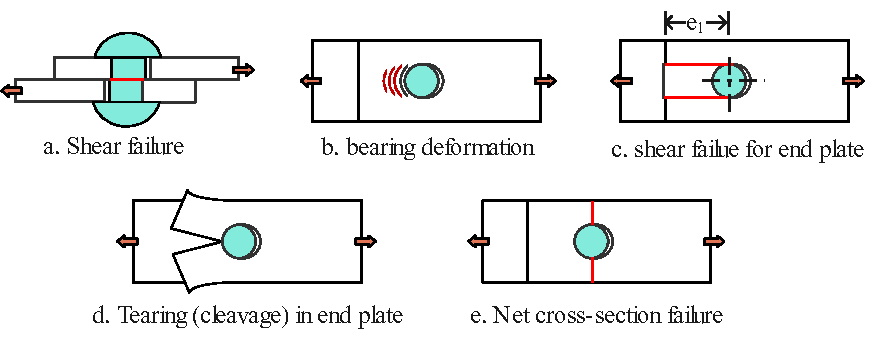
\includegraphics{imgs/ch2/failure-mode-bea.pdf}
    \caption{Failure mode of bearing type connection}
    \label{fig-beafalmode}
\end{figure}

For strength calculations of rivets, refer to Section \ref{secbc} on bearing type bolted connections, where national benchmarks use approximately the same calculation method for both rivets and bolts.


\subsection{Literature review}

Research has shown that riveted connections have been extensively studied in various countries in the past. However, most of the research has focused on the study of sound riveted connections, while studies on the deterioration of connections over time have evaluated the relationship between the structural integrity of the riveted structure and the service life, and have reported on the occurrence of damage and component performance degradation. The residual carrying capacity of corroded riveted beams and the estimation formulas for their carrying capacity have been specifically assessed through experiments and finite element analysis. However, these studies primarily focus on the residual carrying capacity of riveted connections and the residual performance of materials. There is less research on the repair and strengthening methods of riveted bridges, especially when rivets are replaced by high-strength bolts due to corrosion, and the changes in joint performance and load transfer mechanisms are not yet well understood.

\begin{figure}[htbp]
    \centering
    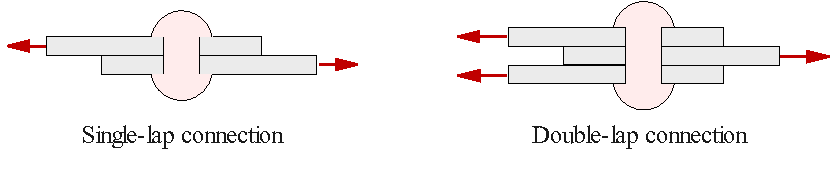
\includegraphics[width=0.85\textwidth]{imgs/ch2/lap-connec.pdf}
    \caption{Single \& Double lap connection}
    \label{fig-lapconnec}
\end{figure}


\begin{figure}[htbp]
    \centering
    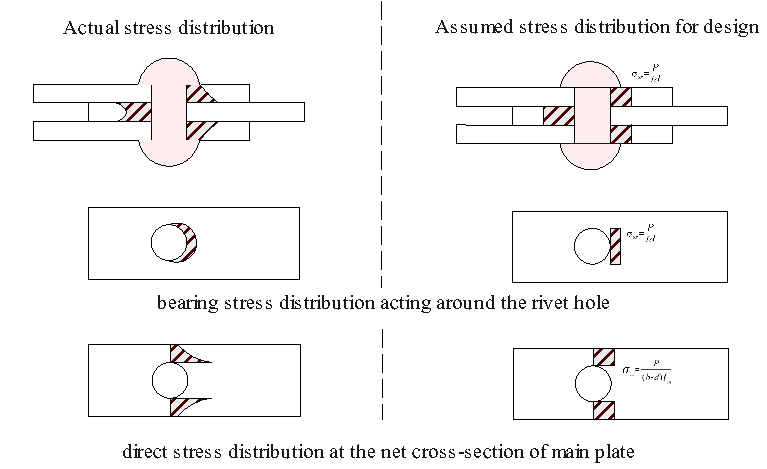
\includegraphics[width=0.85\textwidth]{imgs/ch2/bstressdistr-0.pdf}
    \caption{Stress distribution of double-lap riveted connection}
    \label{fig-rsdisri}
\end{figure}





\subsubsection{Assessment of riveted bridge: fatigue, strength, corrosion}
Extensive research on riveted joints has been conducted in numerous countries in the past. However, the majority of these studies focused on the examination of intact riveted joints. Haghani et al.\cite{haghani2012} conducted a comprehensive review of fatigue damage cases in over 100 bridges. Hołowaty et al. \cite{holowaty2022} examined the structural condition of 13 aged steel bridges constructed between 1873 and 1890, as well as 17 bridges spanning from 1907 to 1983.
Bacinskas et al. \cite{BACINSKAS2013136} conducted a study on the structural condition and behavior of a riveted steel truss bridge using full-scale static and dynamic testing. Aktan et al. \cite{aktan1994destructive} conducted a comprehensive series of nondestructive and destructive tests on two 80-year-old steel truss bridges that had been decommissioned, and the results show that, after completing each destructive test, no evidence of distortion or failure was found in the retrofitted connections. The effectiveness of the retrofit was demonstrated under the heavy concentrated loads experienced during destructive testing. Consequently, it can be deduced that similar bridges can be retrofitted to acceptable levels of safety with minimal effort and cost. Wang et al. \cite{wang2012} conducted a series of tests on an original steel angle obtained from a riveted truss Lanzhou Zhongshan Bridge, which was constructed in 1909. These tests examined the material mechanics, fracture behavior, and fatigue properties of the angle. Kossakowski \cite{kossakowski2013fatigue} presented the research findings on the fatigue strength of steel extracted from a railway bridge that had been in service for over a hundred years. The study focuses on analyzing and investigating the corrosion rate and assessing steel degradation. Małgorzata \cite{Skorupa2015InvestigationJoint} conducted experiments to investigate the load transfer mechanism of single-lap riveted joints and proposed a straightforward model to explain the transfer process. Gocál and Odrobiňák \cite{Gocal2020OnBridges} examines the influence of atmospheric corrosion on the load-carrying capacity of old riveted bridge structures. It analyzes the results and discusses the importance of long-term in situ corrosion measurements, as well as regular inspections for existing bridges. Reichle \cite{Reichle1999} analyzes the behavior of corroded rivets used in the connections of structural steel members. In particular, the material loss caused by corrosion is quantified using finite element analysis. And the findings of a parametric study and offers recommendations for deciding when to replace corroded rivets were presented. Zice \cite{Zice2023} conducted to investigate influences of the corrosion extent of rivet heads with artificial corrosion damage on the mechanical behaviour.

Numerous studies\cite{imam2008,Ryoichi2013,1987163,hisanori1991} have assessed the structural integrity of aging riveted connections in relation to their service life, and have reported on the correlation between the rate of damage and the decline in member performance. Through experiments and \ac{FEM} analyzes\cite{nakata2016, Yurika2019,chen2022jp,cheniabse2022,Pipinato2014ResidualApproach,Bertolesi2021FatigueApproach}, the assessment of the remaining load bearing capacity of corroded riveted girders and the development of formulas for estimating said capacity have also been clarified. 

\subsubsection{Repair and reinforcement}
Lima et al.\cite{lima2008} presented the rehabilitation process of a century-old steel truss bridge with riveted connections in Canada. Kääriäinen \& Pulkkinen \cite{kaaria2002} documented the rehabilitation of the Tornionjoki steel truss bridge. Kimura et al.\cite{kimura2009} performed static loading tests to evaluate the strength of corroded rivet parts as well as the replaced parts using high-strength bolts. These components were obtained from a steel railway bridge that had been decommissioned, as well as from highway bridges. Siwowski \cite{siwowski2013} documented the rehabilitation of a continuous Warren-type steel truss bridge consisting of five spans, constructed in 1961. Gheitasi et al. \cite{Gheitasi2022} documented the rehabilitation of a historic steel truss bridge, which was 133 years old. The rehabilitation process involved partial dismantling, temporary relocation, and retrofitting, with a focus on various aspects of design and construction. Heydarinouri et al. \cite{Heydarinouri2021} presented a retrofit system that utilized pre-stressed CFRP bars to strengthen the double-angle connections between the stringers and floor beams of a riveted railway bridge in Switzerland, which had been in service for 92 years.



\subsection{Clamping force (Preload) of rivet}

When the heated rivet cools and hardens, the shrinkage of the rivet shaft introduces a significantly higher clamping force. In the past, there have been few studies to assess the clamping force of rivets due to limitations in measurement techniques. In the past, it was believed that the rivet would provide a clamping force equivalent to the yield point of the steel \cite{VanMaarschalkerwaart1982FatigueJoints}. However, subsequent experiments have shown that a clamping force of the yield point of the shaft part can be achieved by incorporating a relatively long rivet shaft ($>100 mm$). In contrast, when a short rivet shaft is present, the mean value of the clamping force introduced is lower, and the dispersion is also higher \cite{Zhou1994FatigueMembers, Baron1953TheJoints}. The deviation of the rivet head is believed to have a significant impact on the clamping force for short rivet axes.

Previous research findings \cite{Zhou1994FatigueMembers} indicate that the clamping force is dependent on the steel grade, particularly for rivets with a diameter of 24.5 mm. Therefore, Åkesson \cite{Akesson2010} refers to the nominal tensile stress caused by the clamping force in the axial section of the rivet as the clamping stress. The clamping stress to yield stress ratio of the rivet material was a crucial parameter in assessing the rivet clamping force. The average ratios were 0.61 and 0.77 for the rivet shaft lengths of 75 mm and 125 mm respectively. K{\"u}hn \cite{Kuhn2008AssessmentLife} have shown that the tightening force of st52 material rivets is lower than that of st37 material rivets. Heinemeyer \cite{Heinemeyer2011TheConnections} presents recent investigations on the impact of rivet head corrosion on the pre-stressing of the rivet, achieved through milling the rivet's head and conducting numerical simulations. It also presents fatigue tests that provide initial results for assessing the remaining lifespan of a riveted connection with reduced rivet stress.

The above mentioned previous studies mainly conducted tests in laboratory settings utilizing relatively long rivet shafts. Nevertheless, the actual clamping force introduced during riveting real bridges, particularly in-situ, differs to some extent from these experimental findings due to mistakes made during the riveting operation. A previous study8) removed rivets from real bridge girders and flanges to measure the residual rivet clamping force. Akesson \cite{Akesson2010} and Baron \& Larsson \cite{Baron1953TheJoints} reported comparable outcomes. Both sets of experimental data indicated that the length of the rivet shaft had a significant impact on the clamping force. Fig.\ref{fig-preload-rivet}  showed that a relatively long rivet shaft increased the average clamping force while decreasing its variance. Moreover, Leonetti \cite{Leonetti2020RivetBridges} also found that the number of plates also had an influence on the clamping force of the rivet. The misalignment of the holes of the plates has been reported to be caused by construction errors.

\begin{figure}[htbp]
    \centering
    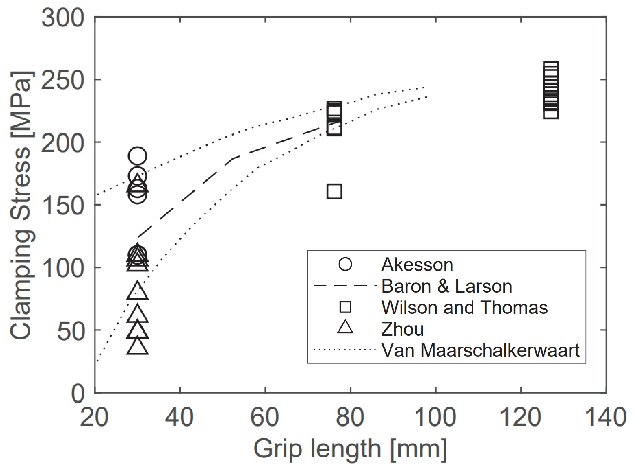
\includegraphics[width=0.8\textwidth]{imgs/ch2/preload-rivet.pdf}
    \caption[The variability of the clamping stress as a function of the grip length for carbon steels.]{The variability of the clamping stress as a function of the grip length for carbon steels. (figure cite from \cite{Leonetti2020RivetBridges}, experimental data from Åkesson \cite{Akesson2010},Wilson and Thomas \cite{Wilson1938FatigueJoints}, and Zhou \cite{Zhou1994FatigueMembers}. Also the average trend from Baron \& Larson \cite{Baron1953TheJoints}, and upper and lower bounds from van Maarschalkerwaart \cite{VanMaarschalkerwaart1982FatigueJoints} are reported.)}
    \label{fig-preload-rivet}
\end{figure}


\subsection{Remaining issue}
However, the primary focus of these studies is on the residual carrying capacity of riveted connections and the residual performance of materials. Insufficient research has been conducted on the repair and strengthening methods of riveted bridges, especially in cases where corrosion leads to the substitution of rivets with high-strength bolts, resulting in limited understanding of the alterations in joint performance and load transfer mechanisms. Steel riveted bridges hold significant cultural and historical value as a part of our constructive heritage from the previous century. Numerous iron and steel riveted bridges are of historical importance, requiring restoration and preservation, and are currently operational.

\section{Friction type bolted connection}

\subsection{Background}

Friction-type High-strength bolt connections have been widely used in building steel structures recently due to their ease of installation, higher bearing capacity, and superior anti-fatigue performance. The high-strength bolt connection can be classified into bearing type and friction type based on the difference in force transmission patterns as shown in \ref{fig-fricandbearing}. In the case of the bearing type, the connection's bearing capacity depends on the resistance of the hole wall and the shear resistance of the bolts. In the case of the friction type, the force is transmitted through friction between the faying surfaces of the plates. The resistance of the bearing type connection is typically higher than that of the friction type. However, the bearing type connection is not directly suitable for fatigue and dynamic loads.

\begin{figure}[htbp]
    \centering
    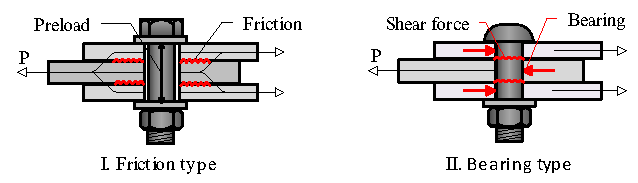
\includegraphics[width=0.85\textwidth]{imgs/ch2/fricandbearing.pdf}
    \caption{Schematic of load transmit mechanism of friction-type and bearing-type bolted connection}
    \label{fig-fricandbearing}
\end{figure}

The mechanical properties of bolted joints have a direct impact on their load-bearing capacity. The spacing, strength, and stress state of bolts all play a crucial role in determining the mechanical properties of high-strength bolted joints. Extensive research has been conducted over the years to investigate the various factors that affect these properties \cite{peng2015,Lyu2019NumericalSteels,Brian1996EdgeOcnnections,wang2020interface,hirashima2004experimental}. This research has helped identify ways to optimize the performance of bolted joints, ensuring the safety and longevity of structures in diverse applications. Understanding the factors that influence these properties enables engineers and designers to make informed decisions regarding material selection and structural design to meet specific performance requirements.

The construction of new bridges often entails several design challenges. Among these challenges is the requirement to enhance the strength of bridge components to withstand increased external live loads, without necessitating a larger overall structure. This necessity for adjustments has gained prominence in recent years, coinciding with the growing utilization of high-strength steels in bridge construction.

To fulfill this requirement, the bolted joints within the steel bridge structure must be engineered to endure the augmented strength of the steel components. However, the strength of friction-type joints is influenced by two primary factors: the quantity of bolts employed and the slip coefficient. 

Increasing the number of bolts is a simple and effective measure. However, an increase in the number of bolts means that the size of the joint will become larger, resulting in added weight. Large joints bring about several disadvantages, such as decreased load-carrying capacity with increasing side length of the joint. Additionally, an increase in the number of bolts complicates the management and maintenance of the bolt group, thereby increasing the maintenance costs of the bridge.

\subsection{Design methods}

%各国设计标准对于slip resistance的计算方法都一样可以通过式子-ch2fs计算得出。然而,对于一些折减系数的定义各国标准略有不同,例如对于孔大小的折减等,这里就不做探讨了。

\begin{equation} \label{ch2fs}
    F_s=\mu m N_0
\end{equation}

where, m is the number of friction planes, $\mu$ is the slip coefficient of faying surface, $N_0$ is the initial preload before loading, $n_0$ also can be calculated by $0.7f_{ub}A_s$

\subsection{Long bolted joint}
As a joint length increases, problems arise when using  long or large bolted joints. First, owing to the presence of secondary members in the vicinity of the joint (e.g., stiffener and diaphragm), excessively long joints can interfere with secondary members. Therefore, it is necessary to shorten the length of the joint while maintaining design strength. Typically, a slip-critical joint combined with a weld is used to satisfy the design strength requirements of a joint. Previous studies have demonstrated that slip-critical bolted joints combined with welds are reliable and feasible \cite{solodov2021,Thomas2000,Chang2019361,KHANDEL2022107036}. Combinations of welded--bolted connections are widely used in steel structures. However, some environments, such as those offering insufficient space or requiring work at height, are not conducive to welding during onsite bridge construction. Welding also destroys the original coating of steel parts, which necessitates repainting the joints. As a result, the construction of combined welded--bolted connections is very difficult for steel bridge joints that require onsite joining. Appropriate methods are required to shorten the bolted joint without reducing its strength. \par

Second, as the length of the joint (defined as the spacing between the first and last fasteners in a joint) increases, the resistance that can bolt provide decreases to a value lower than the slip strength because the distribution of the bolts inside the joint becomes uneven. As the joint length increases with an increasing number of bolts in a line, the differential deformations in the main plate causes shear failure at the end bolts before all bolts can develop their full shearing strength. This ''unbuttoning'' phenomenon has been observed for all types of fasteners including rivets \cite{fisher1965behavior}. Bendigo et al.\cite{bendigo1963long} concluded that for longer connections, end bolts are sheared before all the bolts can develop their full shear strength. For short connections, the average shear stress is approximately 85\% that of a single bolt; however, for a 52.5 inch long connection, bolts only develop 60\% of their strength. Kamei et al. \cite{KAMEI2000} also showed that the serviceability limit strength decreases by approximately 2.5 $\%$ for each additional row.  Tan et al.\cite{Tan2022} considered that when the number of rows of bolts is more than 5, the force transmission ratio of the end bolt is 0.389.

Owing to the above issues, specifications for long-bolted joints, such as AASHTO, Eurocode, as well as Japanese and Chinese, all provide a reduction factor based on the length of the bolted joint\cite{AASHTO2020,eccs1985,isohtb,eurocode3-21,douji2017}. Furthermore, owing to uneven load sharing, the bolts cannot simultaneously fracture, and the ultimate limit bearing capacity decreases \cite{Takai2021BoltUnbuttoning,Peng2013FeaDimensions,peng2010,longstainless2022}. 

The European Convention for Constructional Steelwork (ECCS), and ISO/TC specify that the resistance should be reduced by a factor of $\beta_{rd}$ when the spacing between the first and last bolt in a joint is larger than 15d as shown in Eq.\ref{ch2eq1} \cite{eccs1985,isohtb}. AASHTO \cite{AASHTO2020} provides the nominal shear resistance of bolts in joints longer than 38.0 in. must be reduced by an additional factor of 0.83 or 0.75/0.9\par

\begin{equation}
    \beta_{rd} = \begin{cases}1 & (L \leq 15 d) \\ 1.08-L /(200 d) & (15 d<L \leq 65 d) \\ 0.75 & (65 d<L)\end{cases}
    \label{ch2eq1}
\end{equation}

Eurocode 3 (EN 1993-1-8:2005) \cite{eurocode3-21} provisions that where the distance $L_j$ between the centers of the end fasteners in a joint, measured in the direction of force transfer is more than 15d, the design shear resistance of all the fasteners should be reduced by multiplying it by a reduction factor $\beta_{Lf}$:
\begin{equation}
    \beta_{Lf}=1-\frac{L_j - 15d}{200d}
\end{equation}

Japanese Specification for Highway Bridge (JSHB) \cite{douji2017} published by Japan Road Association states that when the number of row exceeds 8 in bolted joint, a reduction factor must be applied to the slip strength, as shown in Table \ref{tab-jpredu}.
\begin{table}[h]
    \centering
    \caption{Reduction of slip strength of bolted joint of JSHB-JRA}
    \begin{tabular}{cccccc}
    \toprule
        Number of Row &  8 & 9 & 10 & 11 & 12 \\ \midrule
        Reduction factor & 1.00 & 0.98 & 0.96 & 0.94 & 0.92 \\ \bottomrule
    \end{tabular}
    \label{tab-jpredu}
\end{table}

Furthermore, due to the non-uniformity of load distribution, the bolts are unable to fracture simultaneously, consequently leading to a reduction in the ultimate limit bearing capacity.\cite{Takai2021BoltUnbuttoning,Peng2013FeaDimensions,peng2010}.

Considering the installation space requirements and strength problems associated with long-bolted joints, a rational compact joint must be developed to allow the use of fewer bolts to transmit more load, which could also improve the serviceability limit capacity of the joints.

\subsection{Technical Problem}
Problems arise when utilizing long or large friction-type bolted joints as the joint length increases. Firstly, these excessively \ac{long bolted joints} can cause interference with secondary members, such as stiffeners and diaphragms, located in close proximity to the joint as shown in Fig. \ref{fig-boxhsbinter}. Therefore, it becomes necessary to reduce the joint length while maintaining the design strength. Typically, a friction-type bolted joint combined with a weld is employed to meet the design strength requirements of a joint. Previous studies have demonstrated the reliability and feasibility of friction-type bolted joints combined with welds \cite{solodov2021,Thomas2000,Chang2019361,KHANDEL2022107036}. Combinations of welded-bolted connections are sometimes utilized in steel structures to improve their strength. However, However, this combination methods is inefficient in terms of load bearing capacity enhancement, also the certain environments, such as those with limited space or requiring work at height, are not conducive to onsite welding during bridge construction. Additionally, welding destroys the original coating of steel parts, necessitating reapplication of the protective paint to the joints. Consequently, the construction of combined welded-bolted connections for steel bridge joints that require onsite joining becomes highly challenging. Thus, suitable approaches are required to reduce the length of bolted joints without compromising their strength.

\begin{figure}[htbp]
    \centering
    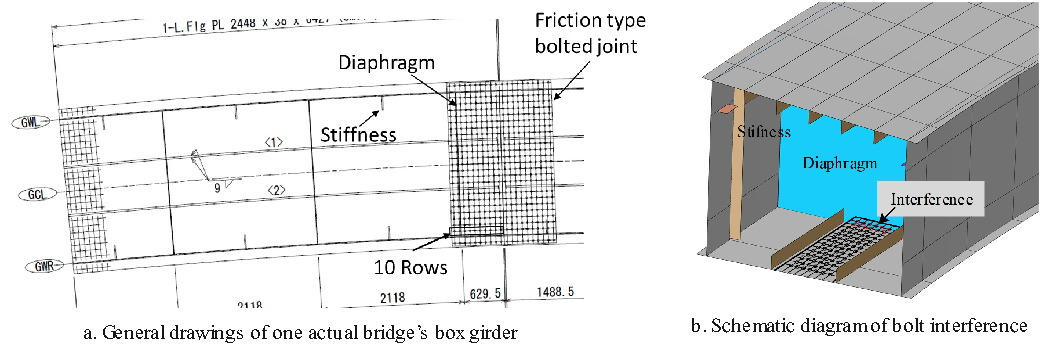
\includegraphics[width=1\linewidth]{imgs//ch2/boxhsbinter.pdf}
    \caption{Actual engineer case of the need of hybrid joint: the joint of box girder}
    \label{fig-boxhsbinter}
\end{figure}

Second, as the length of the joint (defined as the spacing between the first and last fasteners in a joint) increases, the resistance that can bolt provide decreases to a value lower than the slip strength because the distribution of the bolts inside the joint becomes uneven. As the joint length increases with an increasing number of bolts in a line, the differential deformations in the main plate causes shear failure at the end bolts before all bolts can develop their full shearing strength. This "unbuttoning" phenomenon has been observed for all types of fasteners including rivets \cite{fisher1965behavior}. Bendigo et al.\cite{bendigo1963long} concluded that for longer connections, end bolts are sheared before all the bolts can develop their full shear strength. For short connections, the average shear stress is approximately 85\% that of a single bolt; however, for a 52.5 inch long connection, bolts only develop 60\% of their strength. Kamei et al. \cite{KAMEI2000} also showed that the serviceability limit strength decreases by approximately 2.5 $\%$ for each additional row.  Tan et al.\cite{Tan2022} considered that when the number of rows of bolts is more than 5, the force transmission ratio of the end bolt is 0.389.

Owing to the above issues, specifications for long-bolted joints, such as AASHTO \cite{AASHTO2020}, Eurocode3 \cite{eurocode3-21}, as well as Japanese and Chinese, all provide a reduction factor based on the length of the bolted joint \cite{eccs1985,isohtb,douji2017}. Furthermore, owing to uneven load sharing, the bolts cannot simultaneously fracture, and the ultimate limit bearing capacity decreases \cite{Takai2021BoltUnbuttoning,Peng2013FeaDimensions,peng2010,longstainless2022}. 

Considering the installation space requirements and strength problems associated with long-bolted joints, a rational compact joint must be developed to allow the use of fewer bolts to transmit more load, which could also improve the service limit capacity of the joints.

\section{Bearing type bolted connection} \label{secbc}

\subsection{Background}

The HSB bearing type connection is a connection method based on the idea that, as in the case of friction connections, a preload is usually introduced into the bolt and frictional resistance is used for normal loads, while shear resistance of the bolt shaft and bearing resistance of the base metal and the connecting plate are expected for emergency loads, such as an earthquake \cite{rivet1977}. There are four types of bolt that can be used for support connections: those with a shape similar to that of a friction connection, those with an interference fit (hammered-in type), and the resin-injected bolt or the mechanical bolt-rivet. These bolts are characterised by their method of load transmission, relying primarily on bearing against the sides of holes in the fasteners and friction to transmit forces in a hybrid manner.

Bearing bolts operate on a simple mechanical principle: When a load is applied to the connected structure, it induces direct bearing forces on the bolt shank. These forces, in turn, are transferred to the material surrounding the bolt holes by bearing stress. These bolts are not designed to be preloaded; they operate as soon as the load causes the connected elements to press against the bolt. For optimum performance, the hole diameter is made slightly larger than the diameter of the bolt for ease of installation; however, this clearance must be minimal to maintain load transfer without yielding or excessive deformation. ASTM standards \cite{ASTM-bolt} and others provide guidelines for these tolerances to ensure proper function.

In recent years, the use of bearing type connections has been reported\cite{morikawa2002} in cases where the required performance of the friction faying surface is not satisfied, such as in the case of a reinforce method for fatigue cracks at the corner of steel piers, but the number of applications to actual bridge main members is extremely small. 

Although the bearing-type connection can offer much higher strength compared to the friction-type connection \cite{Li2020bbolt,perry1981bearing,kim1999bearing}, it also faces a series of issues such as poor construction performance and high precision requirements, their application comes with inherent challenges. First, the precise required tolerances between the bolts and the holes. Since load transfer depends on the bearing of the bolt against the edge of the hole, any significant misalignment or incorrect size can lead to reduced load capacity or even structural failure. Furthermore, these connections are susceptible to slipping when exposed to dynamic or cyclic loads, necessitating careful consideration of the slip coefficients of the connected materials and the potential for fatigue.

Moreover, in environments prone to corrosion or where long-term durability is a concern, protective measures must be implemented to preserve the integrity of the bearing-type bolts. Regular inspections are vital to detect any signs of wear, corrosion, or loosening that could compromise the connection's integrity.

In summary, it can be expected that in the future bearing type bolts will be a fundamental element in the design of steel structures, offering a balance between strength, ease of assembly and cost effectiveness.

\subsection{Design resistance}

\subsubsection{Bearing resistance at fastener hole}

In Japan, the latest 2017 edition of the \ac{JSHB} by \ac{JRA} \cite{douji2017} states that bearing type connections can be designed according to the service limit, and the serviceability limit state is determined by checking the shear yield strength of the bolt shaft, and the bearing strength of the main plate.

The bearing strength by JSHB shall be taken as:

\begin{equation}
    F_{b,JSHB} = 1.7 f_y dt
\end{equation}

On the other hand, \ac{JSRS} by \ac{RTRI} \cite{rtri2009Design} states that the area subjected to bearing stresses is less likely to experience plastic flow with yielding due to the surrounding restraints, and that strength above the yield point can be expected. The bearing strength is 50\% above the yield point of the jointed material, as shown in Eq. \ref{eqfbjsrs}.

\begin{equation}\label{eqfbjsrs}
    F_{b,JSRS} = 1.5 f_y dt
\end{equation}


Where, $d$ is nominal diameter of the bolt, $t$ is thickness of the main plate, $f_y$ is the yield strength for main plate.

AASHTO MBE \cite{aashtombe2018Manual} states that the design of rivets can be directly referred to \ac{AASHTO} \ac{LRFD} BDS for bearing type connection, and the specifications states that the effective bearing area $A_{b}$ of a fastener is its diameter $d$ multiplied by the thickness of the main plate $t$ on which it rests, and should be designed for strength limit states。 The bearing strengths are as follows:

AASHTO LRFD BDS 9th editions:

When clear distance between fastener hole $L_c$ is not less than 2d, and with a clear end distance $e_1$ not less than 2.0d:

\begin{equation}
    F_{b,AASHTO} = 2.4dtf_u
\end{equation}

When fastener spacing $L_c$ is less than 2d, and with a clear end distance $e_1$ less than 2.0d:
\begin{equation}
    F_{b,AASHTO} = 1.2L_ctf_u
\end{equation}

Where, $f_u$ is tensile strength stress for the main plate, $L_c$ is clear distance between fastener holes, $e_1$ is the distance between end of plate and the end fastener hole center.

Eurocode 3 \cite{eurocode3-21} states that the bearing type connection (Category A) should be design as ultimate limit state \cite{ec1993-1-1-2020} and can be used without regard to the application of preload and the requirements of the joint faying surface, and that the bearing strength of the bearing type connection can be calculated in accordance with the following formula:

\begin{equation}
    F_{b,EC3} = k_m\alpha_bf_udt
\end{equation}

Where, for steel grades equal to or higher than S460 $k_m$ is 0.9, otherwise $k_m$ is 1

- for end bolts: $\quad \alpha_{\mathrm{b}}=\min \left(\frac{e_1}{d_0} ; 3 \frac{f_{\mathrm{ub}}}{f_{\mathrm{u}}} ; 3\right)$

- for inner bolts: $\quad \alpha_{\mathrm{b}}=\min \left(\frac{p_1}{d_0}-\frac{1}{2} ; 3 \frac{f_{\mathrm{ub}}}{f_{\mathrm{u}}} ; 3\right)$

The Chinese national standard of steel structure \ac{CSSS} GB50017-2017 \cite{gb50017-2017} stipulates that the SLS of bearing type connection can be used in accordance with the friction type connection calculation, while the bearing strength $F_{b,CS}$ is stipulated as the strength limit state, which can be obtained by the following formula calculation:

\begin{equation}
    F_{b,CS}=1.26 f_u dt
\end{equation}

\subsubsection{Shear resistance at fastener shaft}

The \ac{JSHB} stipulates that the shear strength of the bearing type connection for the main plate can be designed as the Serviceability limit strength and Ultimate limit strength respectively, which are calculated by the following formula.

For the SLS:

\begin{equation}
    F_{vf,JSHB,SLS} = f_{yf}/\sqrt{3}A_s
\end{equation}

For the ULS:

\begin{equation}
    F_{vf,JSHB,ULS} = f_{uf}/\sqrt{3}A_s
\end{equation}


Where, $f_{yf}$ is the yield strength stress of fastener. $f_{uf}$ is the ultimate strength stress of fastener. $A_s$ is the effective area of fastener shaft, can be calculated as $A_s = \frac{\pi d^2}{4}$.

\ac{AASHTO} \cite{AASHTO2020} state that the nominal shear resistance of a HSB at ultimate limit state in joints whose length between extreme fasteners measured parallel to the line of action of the force is less than or equal to 38.0 in. And the nominal shear resistance of bolts in joints longer than 38.0 in. must be further reduced by an additional factor of 0.83 or 0.75/0.90.
The shear resistance at fastener shaft can be calculate as following formula:

- Where threads are excluded from the shear plane:

\begin{equation}
    F_{vf,AASHTO} = 0.56f_{uf}A_s
\end{equation}

- Where threads are include in the shear plane:

\begin{equation}
    F_{vf,AASHTO} = 0.45f_{uf}A_s
\end{equation}

Eurocode 3 states that the  shear resistance at fastener shaft can be calculate as following formula:

- Where threads are excluded from the shear plane:
\begin{equation}
    F_{vf,EC3} = \alpha_v f_{uf}A_s
\end{equation}

- Where threads are excluded from the shear plane (Rivets are also calculated according to this formula):
\begin{equation}
    F_{vf,EC3} = 0.6 f_{uf}A_s
\end{equation}

Where, For property of the bolt is classes 4.6, 5.6 and 8.8, $\alpha_v$ is 0.6. For property of the bolt is classes 4.8, 5.8 and 10.9, $\alpha_v$ is 0.5.

Chinese standrad \cite{gb50017-2017} \ac{CSSS} states that the  shear resistance at fastener shaft can be calculate as following formula:

\begin{equation}
    F_{vf,CSSS} = 0.3 f_{uf}A_s
\end{equation}

Where, when the bolt class is lower or equal to the class 8.8, the shear resistance should be taken as $0.4f_{uf}A_s$


\subsubsection{Shear resistance at main plate}

In addition to calculating the above two types of resistance of bearing, the general calculation of load bearing strength should also confirm that the main plate will not occur in the end shear failure, the main plate should be prevented from occurring in Fig. \ref{fig-beafalmode}, such as c. end shear, and d. end tearing failure occurs.

The \ac{AIJ} \cite{AIJ2012AIJStructures} provides two methods for calculating the edge shear resistance $F_{vp,AIJ-1}$ : one is to calculate the shear plane based on the effective cross-sectional area $A_{vp}$, and the other is to calculate it based on the equivalent shear cross-sectional area $A_{vp2}$.

- For the effective cross-sectional area:

\begin{equation}
    F_{vp1,AIJ-ef} = 0.5 A_{vp}f_u
\end{equation}
Where, 

\begin{equation}
    A_{vp} = 2 {e_1 + (n-1)p}t
\end{equation}

- For the equivalent cross-sectional area:

\begin{equation}
    F_{vp1,AIJ-2} = A_{vp2}\sqrt{3}f_u
\end{equation}

Where,

\begin{equation}
A_{vp2}=2\left[\left\{e_1-\frac{\sqrt{2}-1}{2} d\right\}+\left\{p_1+(\sqrt{2}-1) d\right\}(n-1)\right] t
\end{equation}

On the other hand, Kulak \cite{Kulak1988guide} states that the maximum bearing capacity can be expressed by the following Eq. \ref{eqfkulak} based on the experimental results of end-failure joints. The reason why an upper limit is specified for the maximum proof stress is that the failure mode is not end failure (Fig. \ref{fig-beafalmode}-c) but bearing failure (Fig. \ref{fig-beafalmode}-b) when the load exceeds this limit.

\begin{equation}\label{eqfkulak}
    F_{vp,kulak}=2t(e_1-2/d)(0.7f_u)
\end{equation}

\begin{equation}
    F_{b,kulak}=3dtf_fu
\end{equation}

The definition of each symbol for the joint is shown in the following Fig. \ref{fig-symbol}.

\begin{figure}[htbp]
    \centering
    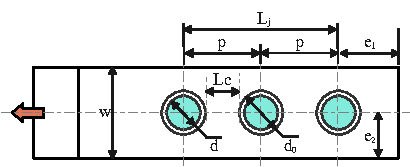
\includegraphics[width=0.7\linewidth]{imgs//ch2/symbol.pdf}
    \caption{The use of the symbols}
    \label{fig-symbol}
\end{figure}

Eurocode 3 also state that the block tearing should be avoided. For a bolt group where the tension stress on the tension area is uniform as shown in Fig. \ref{ch2figeu5-13}, the design block tearing resistance $v_{eff,1}$ should be taken as:

\begin{equation}
    v=[A_{nt}f_u+min(\frac{A_{gv}f_y}{\sqrt{3}}; \frac{A_{nv}f_u}{\sqrt{3}})]/\gamma_{M2}
\end{equation}

where, $A_{nt}$ is the net area subjected to tension, $A_{gv}$ is the gross area subjected to shear, $A_{nv}$ is the net area subjected to shear.

\begin{figure}[htbp]
    \centering
    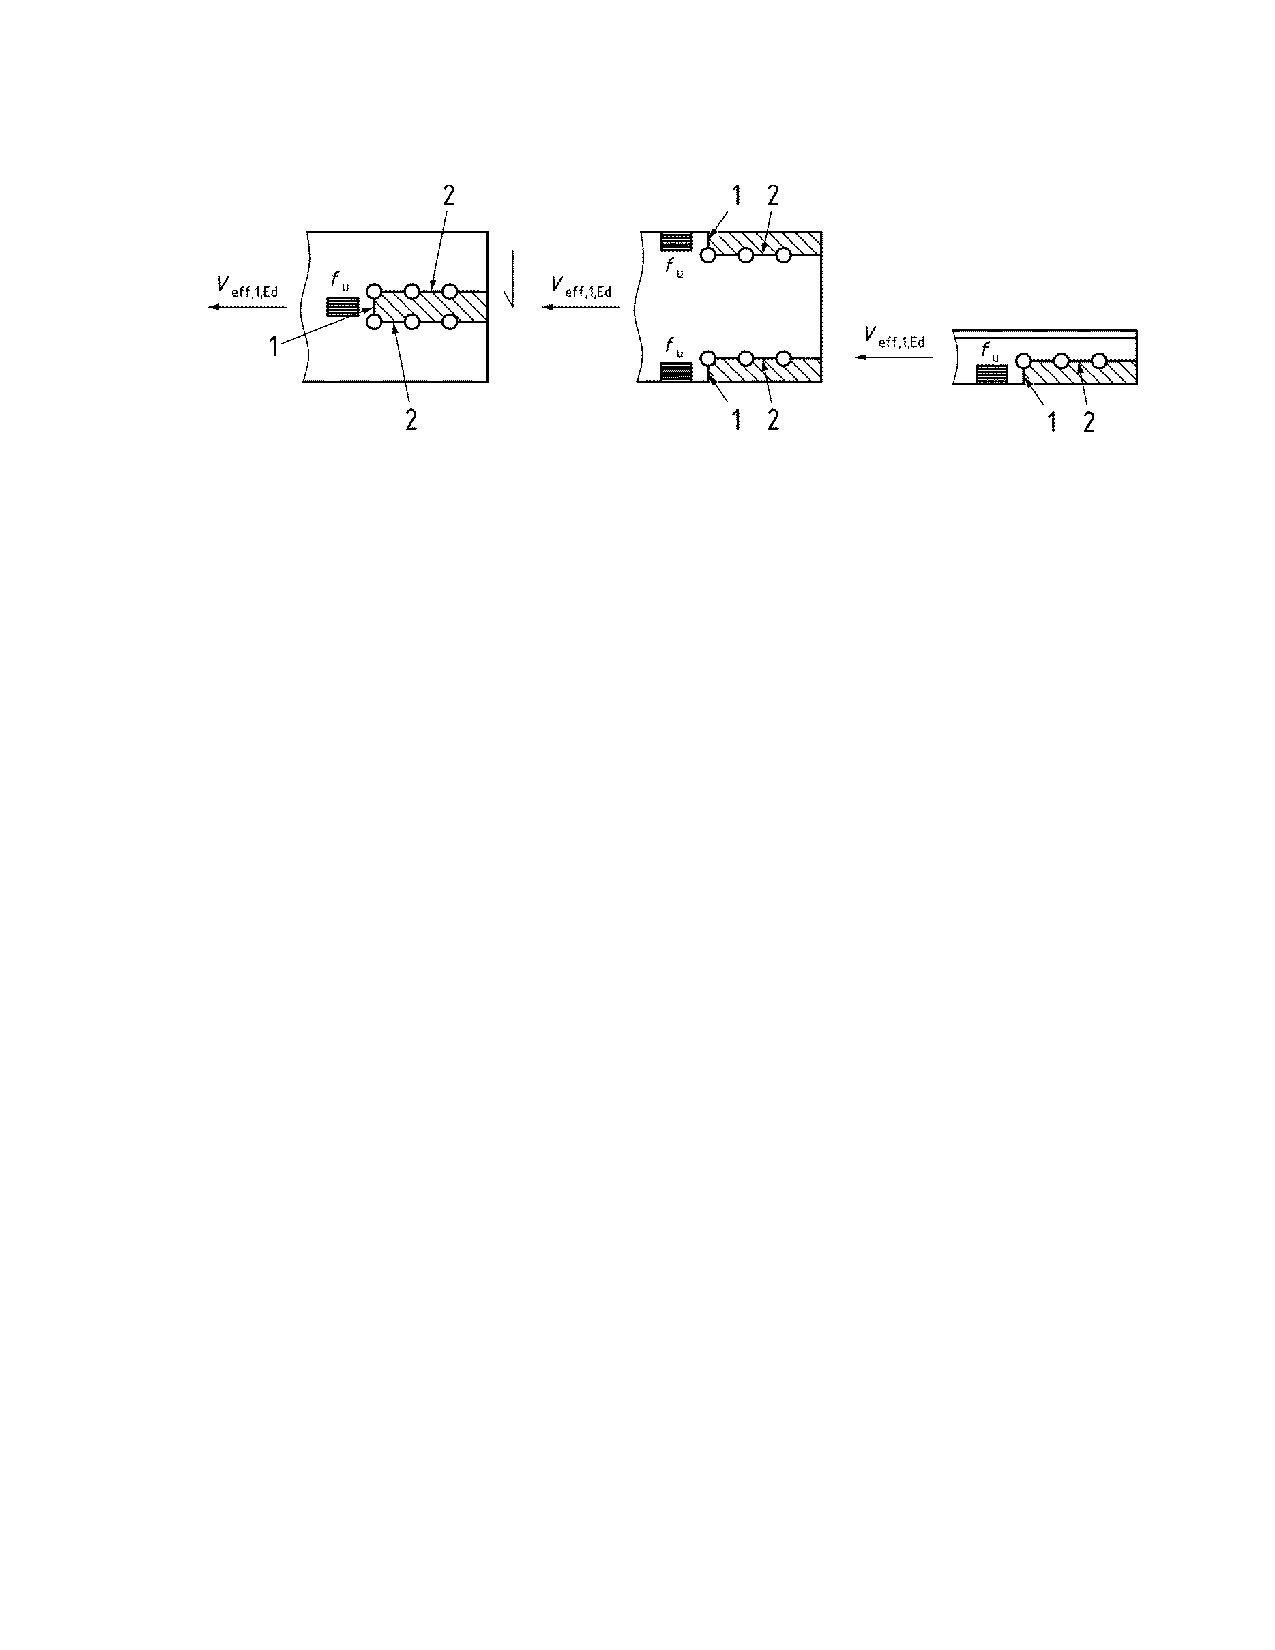
\includegraphics[width=0.7\linewidth]{imgs/ch2/ch2figeu5-13.pdf}
    \caption{The use of the symbols \cite{eurocode3-21}}
    \label{ch2figeu5-13}
\end{figure}


\subsection{Interference fit bolt}

A specialized high-strength bolt for bearing-type connection is present, the bolt have rib around the bolt shaft, the outermost diameter include rib should be over than the bolt hole, so when hanmer into the bolt, the rib will have occur plastic deformation and general interference fit effect, hereafter known as the Interference fit bolt \cite{Kulak1988guide,bolt-bearing,Chen2023MechanicalConnections} as shown in Fig. \ref{fig-onebbolt-ch1}. The B10T grade interference fit bolts were used (courtesy of Kobelco Bolt, Ltd.) and meets the strength requirements of an F10T bolt according to the JIS-B1186 standard \cite{jis2018JIS}, which is equivalent to ASTM-A490 \cite{ASTM-bolt} \& Grade 10.9 \cite{ISO-bolt} and possesses the unique feature of an axially ribbed shank. When the bolt is hammered into a hole, the rib undergoes plastic deformation to ensure a tight fit and prevents excessive slipping. Interference fitting bolts are used to retrofit steel bridge piers that have fatigue damage or corrosion by attaching the patch plate \cite{Anami-bbolt-ate}. This is because initial imperfections or corrosion leads to uneven steel plate surfaces, making it impossible for the patch plate of the friction type bolted connection to effectively contact the steel surface and transmit force. And Interference fit bolts also can reduce the fatigue damage in bolt holes, and increasing their fatigue strength \cite{Guo20205}. However, interference fit bolts are rarely used on other bridge parts due to their stringent installation requirements. 

\begin{figure}[htbp]
    \centering
    \includegraphics[width=0.7\linewidth]{imgs/ch2/oneBbolt.png}
    \caption{Bearing-type Inteference fit bolt (M22, Diameter = 23.5mm), Made in Kobelco Bolt, Ltd.}
    \label{fig-onebbolt-ch1}
\end{figure}

Fig.\ref{fig-cs-b1} shows the cross-sectional diagram of the inteference fit bolt, The cross-sectional diagram was obtained from the hybrid joint that underwent a load of up to 1800kN. Revealing that the deformation of the rib on the non-bearing side is very small as observed in the magnified portion of bolt \#1 on the right side. It has been discovered that despite accurately drilled bolt holes, the interference fit of the rib is not behaving as expected, resulting in a small gap that directly impacts load transfer efficiency. The method of interference fit requires further exploration.

\begin{figure}[htbp]
    \centering
    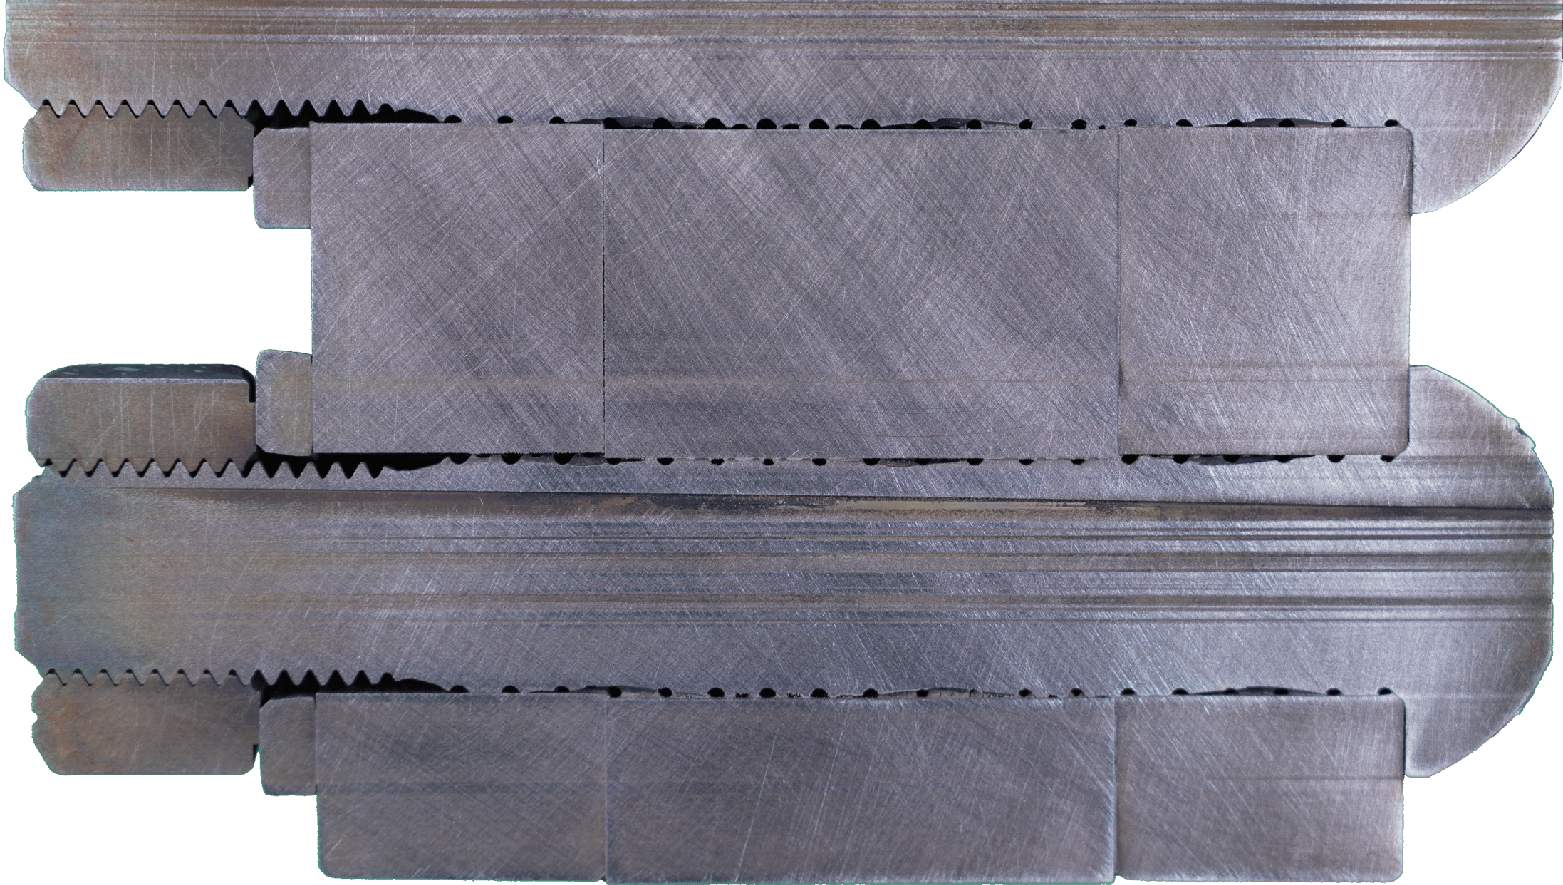
\includegraphics[width=0.8\linewidth]{imgs/ch2/cs-b1.pdf}
    \caption{Sawed-throug cross-section view of interference fit bolt}
    \label{fig-cs-b1}
\end{figure}

Eurocode 3 state that the fit bolt should be desgined using the same methods as the normal High strength bolt,
CSSS consider the bearing resistance of the fit bolt could be expected, the fit bolt also could be using slip resistance designed as the serviceability limit state.

In the JSHB, there only have bearing type connection design methods, but not for interference fit bot, for more effectively use this bolt to provide higher resistance.


\subsection{Resin injected bolt}

Resin-injected bolts are fasteners in which the gap created by the clearance between the bolt and the wall of the hole is filled with a two-component resin as shown in \ref{fig-resinbolt}. They are an effective alternative for bolts fitted with high-strength friction grip bolts in shear connections where slip is not allowed. Injection bolts are a reliable and relatively low-cost option for repairing and improving existing structures \cite{gresnigt1996injbolt}. They are also being used successfully in constructing new structures. The clearance of an injection bolt is filled via a small hole in its head. Once the resin injection is complete and cures completely, the connection becomes slip-resistant. Bearing and shear of the bolt transfer the shear load. In addition, standard structural bolts can be used to fabricate injection bolts. The bolts and washers have been modified to facilitate the injection of resin. The recommendations of ECCS and the Eurocode3 \cite{eurocode3-21,EN14399}for executing steel structures establish the design and execution regulations for injection bolts.

This particular bolt is utilized and analyzed in Europe \cite{pedrosa2022injbolt-mec,kolstein2017injbolt-mec,pedrosa2020injbolt-fati,pedrosa2021injbolt-fati,gresnigt2000injtbolt-use,ungermann2023injbolt-mec}; however, there is no examination or usage of it in Asia. A small quantity of research exists regarding this bolt type within Japan \cite{fujino2010resbolt,Ryota2018resbolt}.

\begin{figure}[htbp]
    \centering
    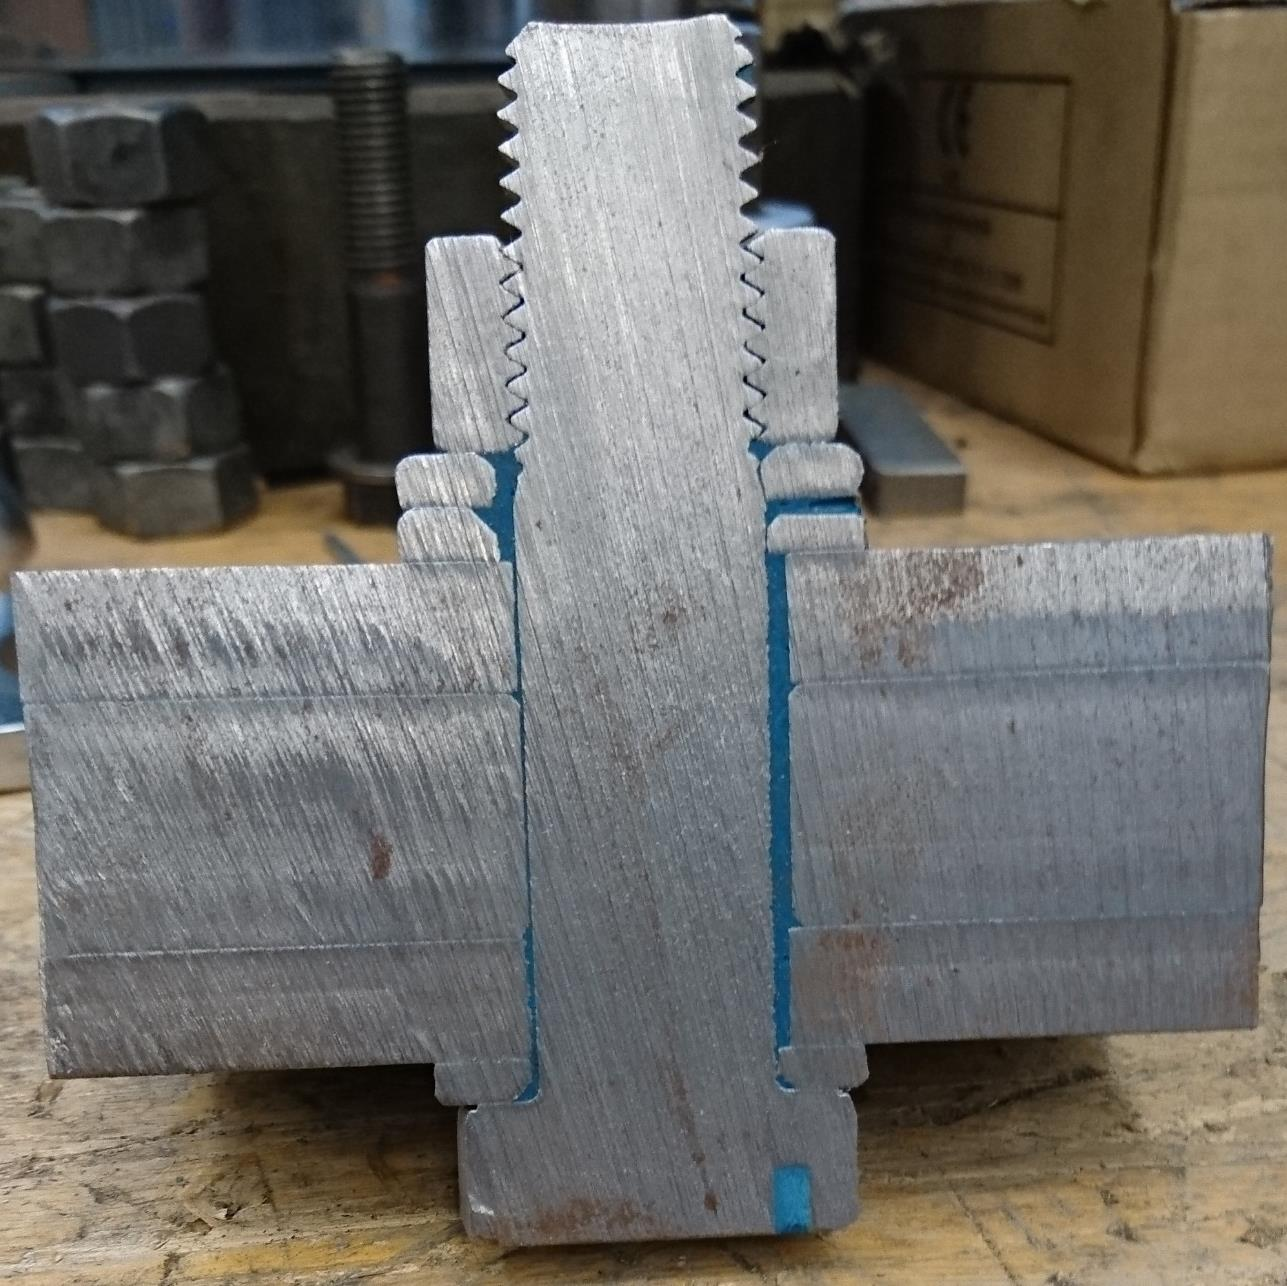
\includegraphics[width=0.65\linewidth]{imgs//ch2/resin-bolt.jpg}
    \caption{Sawed-through (resin) injection bolt connection \cite{Axel2017injbolt}}
    \label{fig-resinbolt}
\end{figure}

\subsubsection{resistance for the resin injection bolt}

For the resin injection bolt, Eurocode 3 state that the strength could be calclutated by sum of 
bearing resistance for the resin and the slip resistance. Although this equation still should be improve, because the resistance between slip and bearing could not simply add, such as the effect of load sharing.


\begin{equation}
    F_{Rd,ser,EC3}=F_s+F_{b,resin}
\end{equation}   

The bearing resistance of resin shall taken as:

\begin{equation}
    F_{b,resin}=\beta dt_{b,resin}f_{b,resin}
\end{equation}

where, $\beta$ is a coefficient depending on the thickness ratio of the main plates. $t_{b,resin}$ is the effective bearing thickness of the resin. 


\subsection{Other: Mechanical bearing blind rivet-bolt}

The above two types of bolted connections have been used in actual steel construction, in addition to these two types of connection, this year Nakamoto et al. (2022) \cite{Nakamoto2022MBBRB} also proposed the \ac{MBBRB}, which can be installed on one side and transmits the load through the bearing force between the bolt and the wall of the bolt hole, as well as the friction force on the joint surface as shown in Fig. \ref{fig-MBBRB}. The load-displacement relationship of the \ac{MBBRB} is equivalent to that of the frictional joint using M22F8T up to the slip load. Therefore, the same service limit state can be applied to the MBBRB joint as to the frictional joint.


\begin{figure}[htbp]
    \centering
    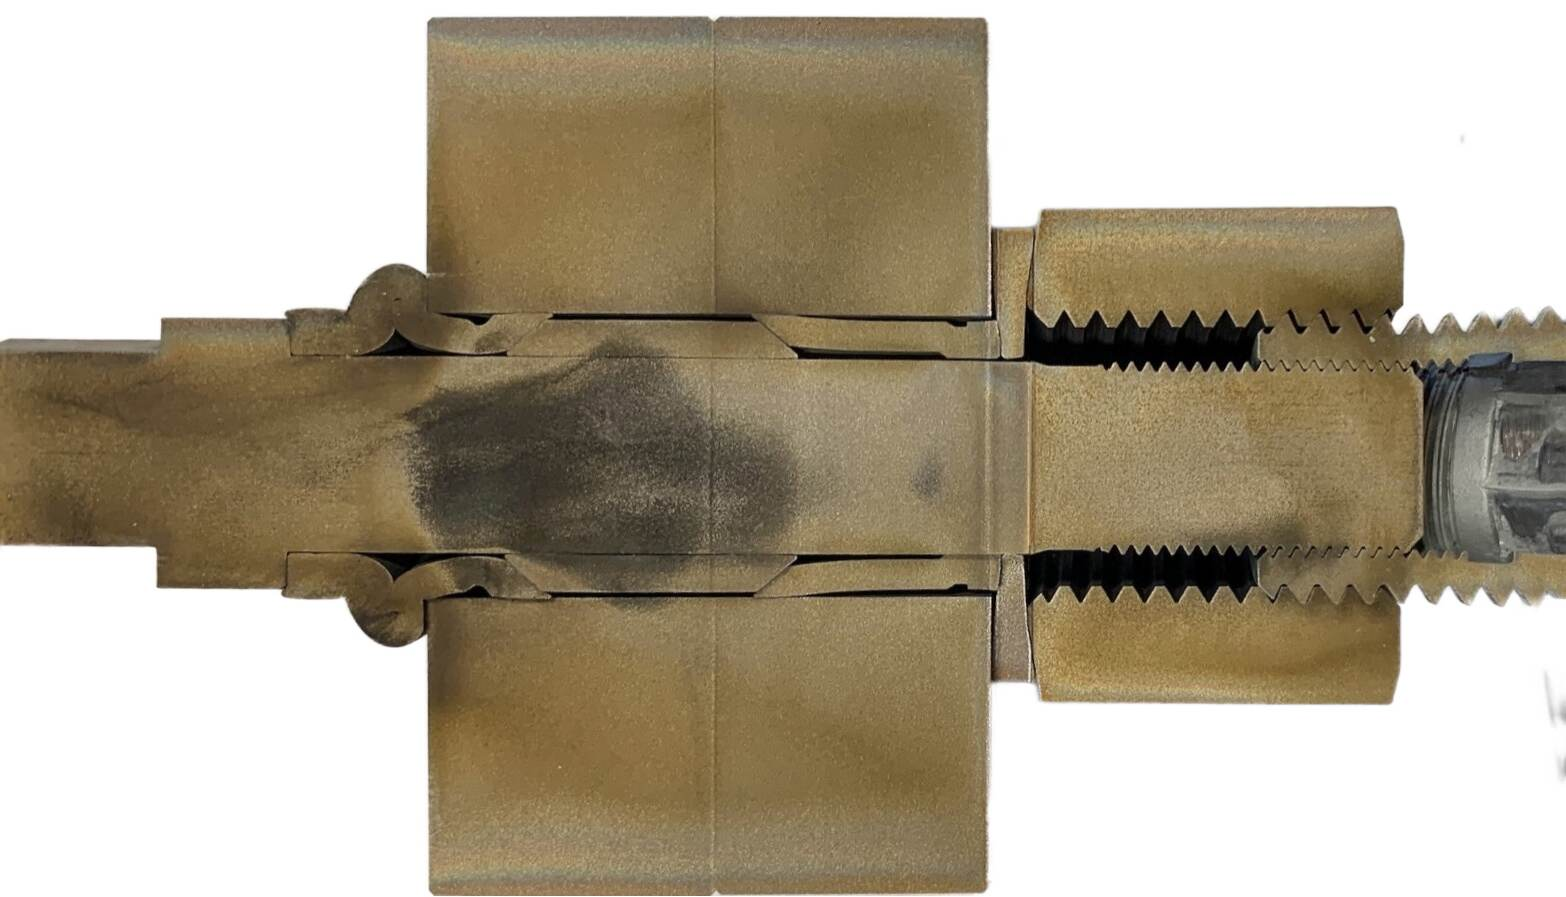
\includegraphics[width=0.85\linewidth]{imgs//ch2/onesidebearingbolt.jpg}
    \caption{Cross-section view of Mechanical Bearing Blind Rivet-Bolts}
    \label{fig-MBBRB}
\end{figure}


\section{Hybrid joint}

Joints are usually made of the same type of fastener, however, in some cases two fasteners with different load transmission mechanisms are assembled on the same joint, which is often referred to as a combination joint or hybrid joint.

The earliest research into hybrid joint was carried out after 1950, when high-strength bolts and welding technology became available as shown in Fig. \ref{fig-schehyb}. Due to the deterioration of riveted bridges, repair work was carried out on riveted connections, and high-strength bolts with better structural performance became one of the alternatives, but the prevailing view at the time was that connections with different mechanical load transfer mechanisms should not be combined, and, in addition, the prevailing research focused on discussing the performance of high-strength bolts and welds.

\begin{figure}[htbp][ht]
    \centering
    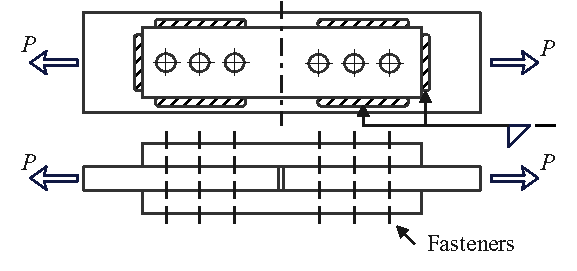
\includegraphics[width=0.75\linewidth]{imgs//ch2/hybrid-sche.pdf}
    \caption{Schematic diagram of Double cover butt hybrid joint (Welding-fasteners)}
    \label{fig-schehyb}
\end{figure}

\subsection{Example of application of hybrid joint}

Aging rivets need to be replaced due to factors such as corrosion of the rivet head and loosening of rivets caused by repeated loading. Despite the requirement for repairs and maintenance of riveted bridges, replacement of original rivets with new ones is not preferred due to the loss of riveting technology and poor constructability of the rivets. In Japan, the use of HSB to replace rivets and form hybrid joints is a common method. Although there are numerous issues that need to be addressed, such as determining the reliability of the slip coefficient of the faying surface and clarifying the mechanism of load transmission. Fig.\ref{fig-bridrivhsb} shows a riveted bridge that is undergoing repair with a mixture of rivets and high-strength bolts. Generally, the original rivets will be removed first, and depending on the situation, it will be chosen whether to replace the cover plate or not, and if necessary, some simple sandblasting and grinding will be performed on the connection surface in order to improve the slip coefficient of the connection surface, and finally the installation of high-strength bolts will be carried out.

%
\begin{figure}[htbp][ht]
    \centering
    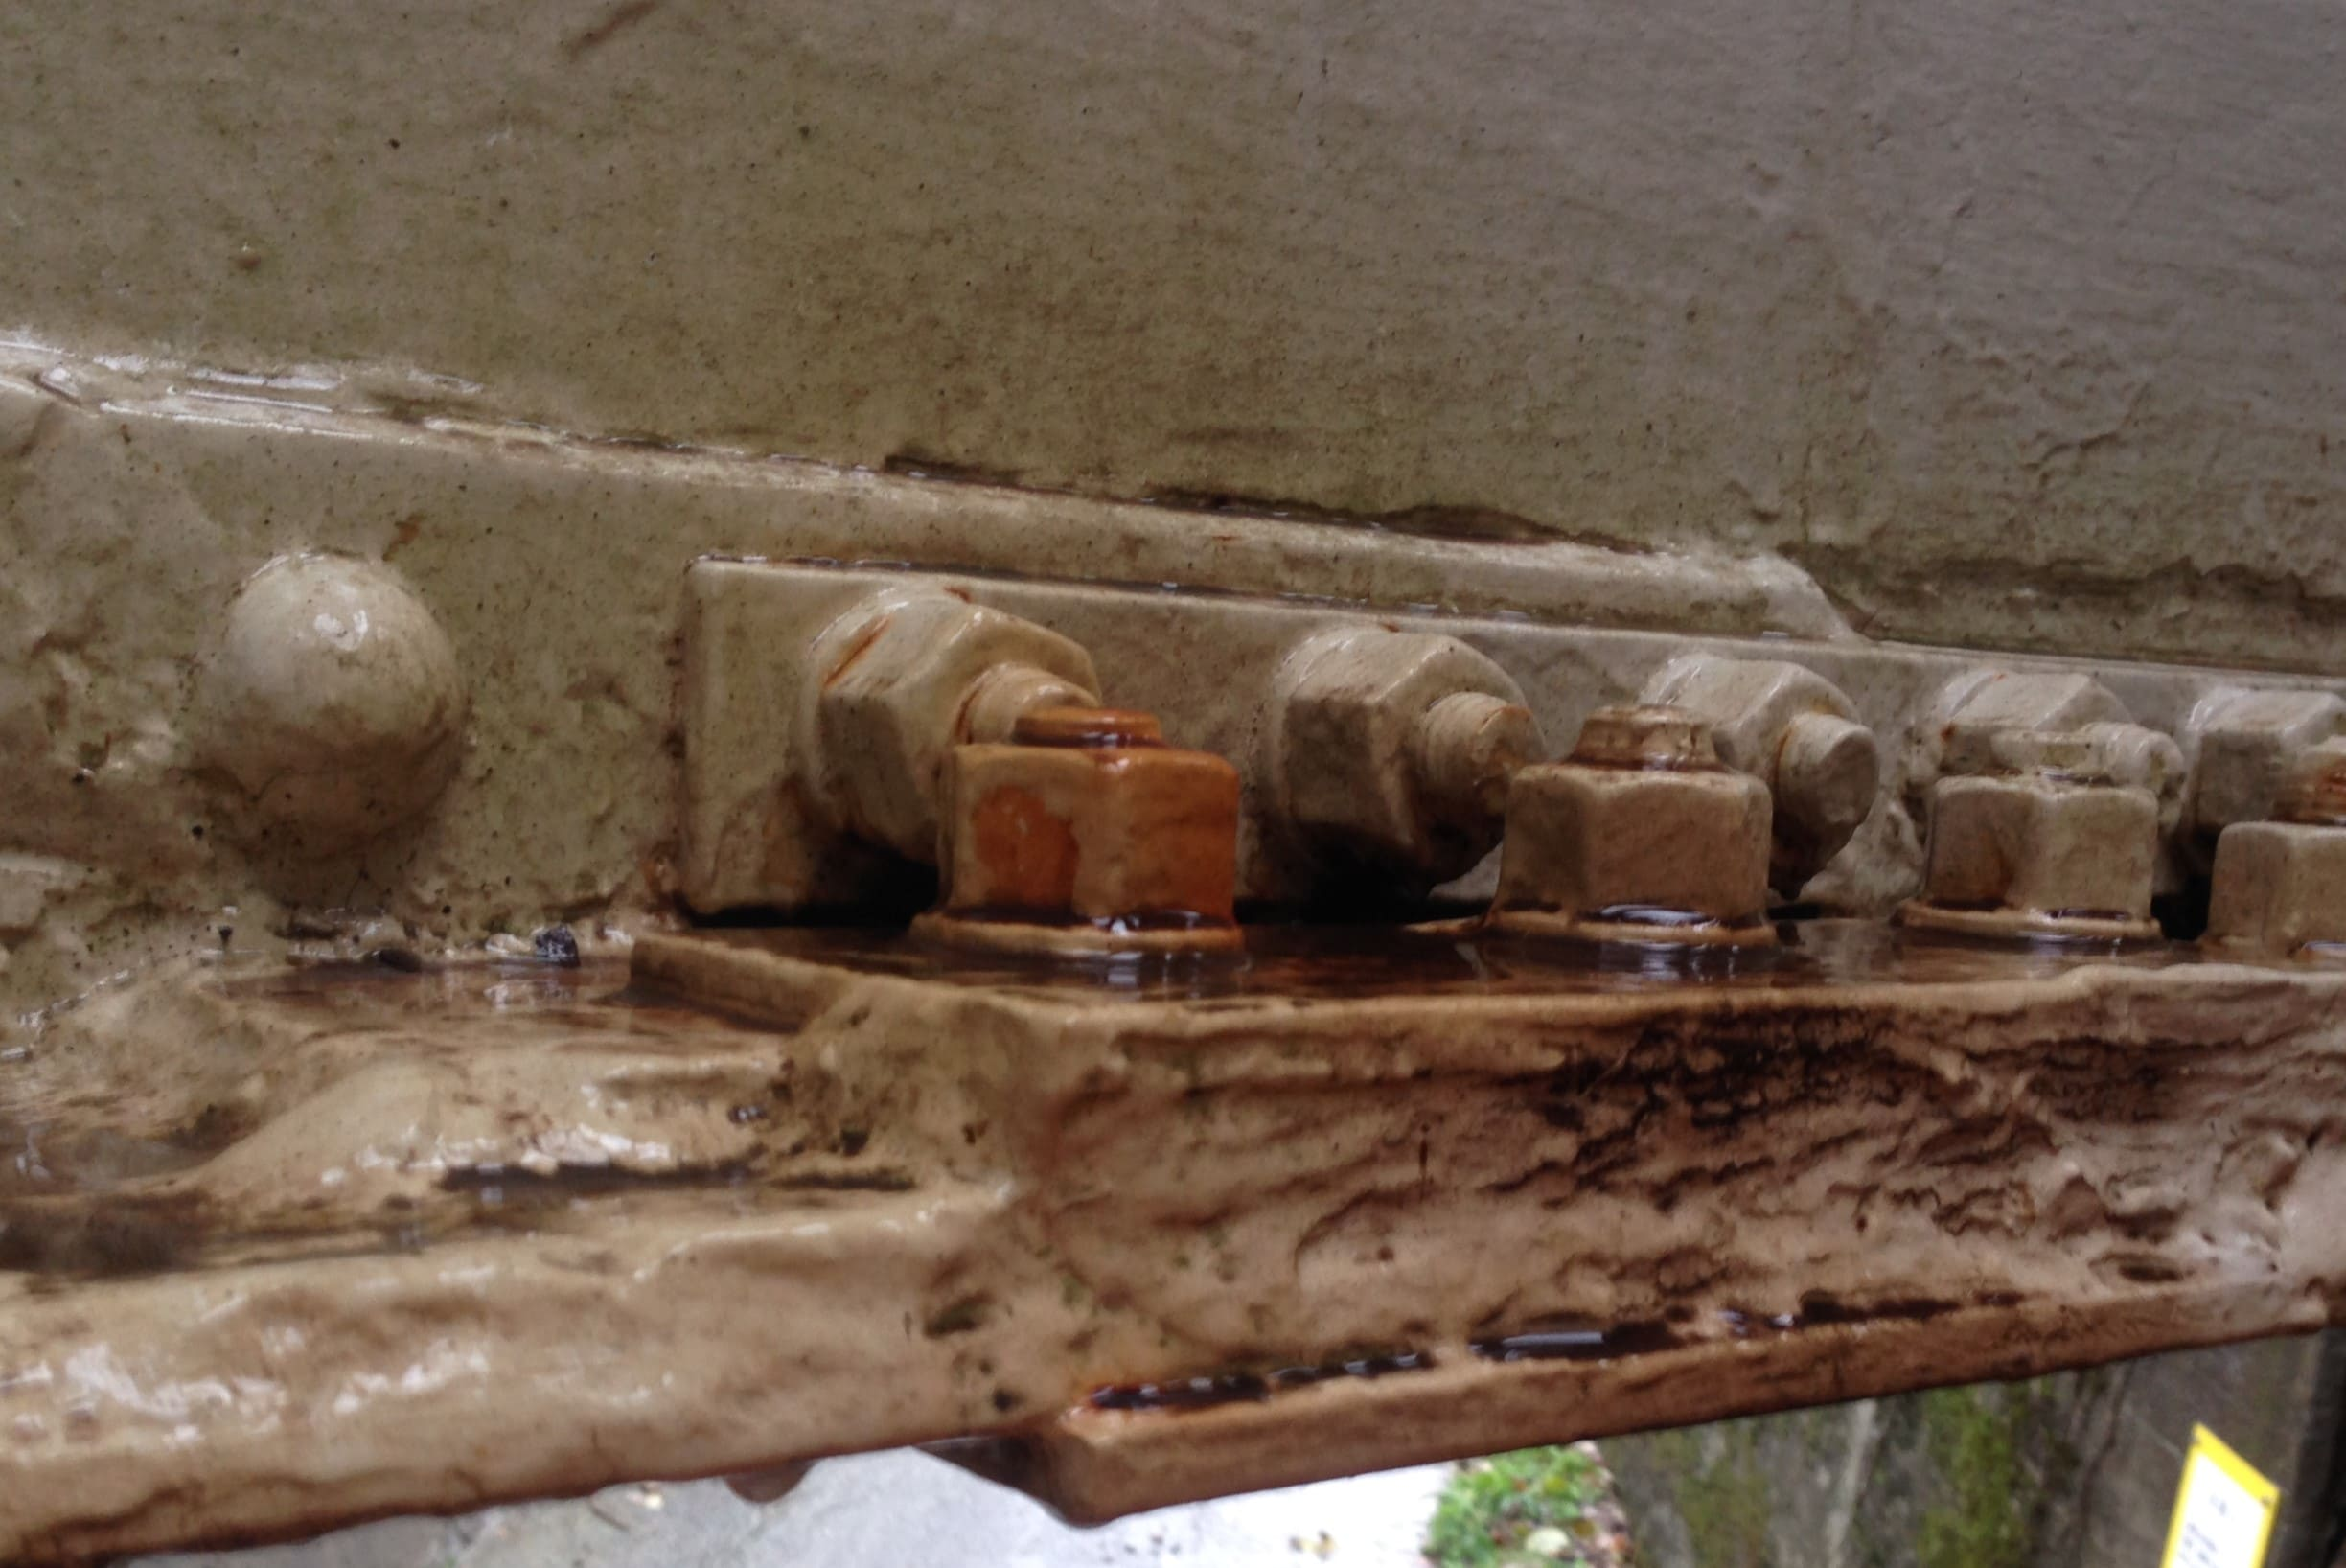
\includegraphics[width=0.75\linewidth]{imgs//ch2/bridge-rivet-HSB.jpg}
    \caption{Riveted joint combined with high-strength bolts. (Hazukawa riveted bridge, Fukui, Japan)}
    \label{fig-bridrivhsb}
\end{figure}

On the other hand, interference fits bolt are also being examined as an alternative to rivets. Substituting the rivets with fasteners that are also transmit load by bearing would have been a more practical option. However, there have a serious problem is that when drilling out the rivets, the original rivet holes have to be slightly enlarged, making it difficult for the IFBs to produce an interference fit effectively. Additionally, due to the precision requirements of the IF bolts, it is challenging to employ them as substitutes for the rivets in fact engineering.

When replacing rivets, it may be necessary to adjust the length of the joint to accommodate the possible addition of extra bolts to enhance its strength. However, the limited space within the bridge girder and the geometry of its components may render the installation of additional bolts impossible, the use of welds to increase the strength of the joint is usually considered in this case \cite{Thomas2000}.

For riveted and welded joints, Bryla(1932)\cite{bryla1932Tests} conducted the first test of hybrid riveted and welded joints but considered only the ultimate strength of the joints. Consideration of riveted and welded fits from the point of view of ultimate strength only does not establish a factor of safety for the strength of the joints. More studies on load distribution followed by Sakurai(1951) \cite{sakurai1951Experimental}, discussing the effects of the construction sequence of riveted and welded joints as well as of the coefficients of the load distribution of riveted and welded joints.

Welding and riveting can share a significant amount of load if handled properly, and the weld has sufficient stiffness and strength to transfer loads other than those originally shared by the rivet, and this type of reinforcement is considered effective \cite{young1934Relative,hiroshi2001Experimental,meier2000composite}. However, the reality is that in the case of old riveted bridges, the steel of the time contained more impurities, i.e. the steel of old riveted bridges is not suitable for welding, and due to the corrosion that often accompanies it, it is difficult to carry out high quality welding work in the field, which directly affects the tensile and fatigue strength of the weld, and therefore welding is not recommended for strengthening riveted bridges, except in special circumstances.

\subsection{Rivets with HSBs}

The incorporation of high-strength bolts into a riveted connection yields various enhancements. In terms of a specific diameter, a high-strength bolt demonstrates superior shear strength compared to a rivet, thereby leading to an overall increase in the ultimate strength of the entire connection. Additionally, the inclusion of high-strength bolts contributes to an augmented stiffness in slip-resistant connections. In the event that slip resistance is surpassed, the presence of rivets, which possess narrower hole clearances relative to high-strength bolts, restricts the occurrence of slip in relation to a fully-bolted joint. Furthermore, research has substantiated that substituting rivets with high-strength bolts enhances the fatigue strength of the joint \cite{reemsnyder1975Fatigue}.

\subsubsection{Mechanical behavior}

Experiments conducted to assess the load-deformation characteristics of short bolted-riveted hybrid joints have revealed that the total resistance offered by the joint can be adequately estimated by summing up the individual resistances provided by the two different types of fasteners.

Komatsu et al.\cite{KOMATSU2015} conducted tensile load tests and chemical tests on aged steel to understand its fundamental properties. Furthermore, tensile loading tests were performed on multi-bolted joints to investigate the replacement of rivets with HSB. The test results reveal that the load carrying capacity and deformability of the partially and fully replaced HSB. joints can be enhanced by introducing frictional resistance, compared to riveted joints alone.

Fig.\ref{fig-hsbriv-fune} \cite{funahashi1967Experimental} and Fig.\ref{fig-hsbriv-stei} \cite{steinhardt1969-hybrid} show typical load versus deformation curves for welded, bolted, and riveted tension specimens. This figure indicates that high-strength bolted connections with normal hole clearance provide a very high initial stiffness up to the slip load of the connection. During slip, the deformations increase significantly until the bolts come into bearing. After the bolts are in bearing, the load versus deformation curve shows an increase in joint stiffness. Joint slip can be minimized by installing fitted bolts in matching drilled holes.

\begin{figure}[htbp]
    \centering
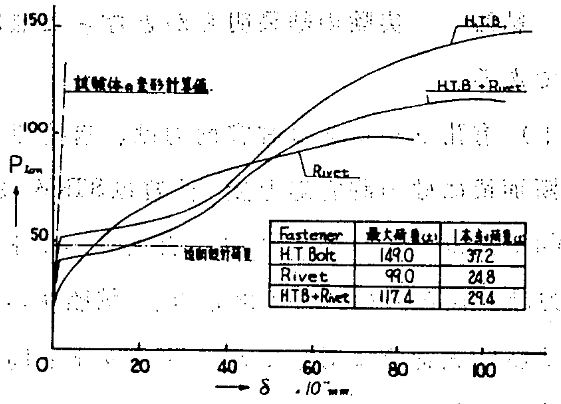
\includegraphics[width=0.75\linewidth]{imgs//ch2/hsbrivet-1967-pd.png}
    \caption{Relationship between load and deformation of Hybrid joint combined with 2 HSB and 2 rivet \cite{funahashi1967Experimental}}
    \label{fig-hsbriv-fune}
\end{figure}

\begin{figure}[htbp]
    \centering
    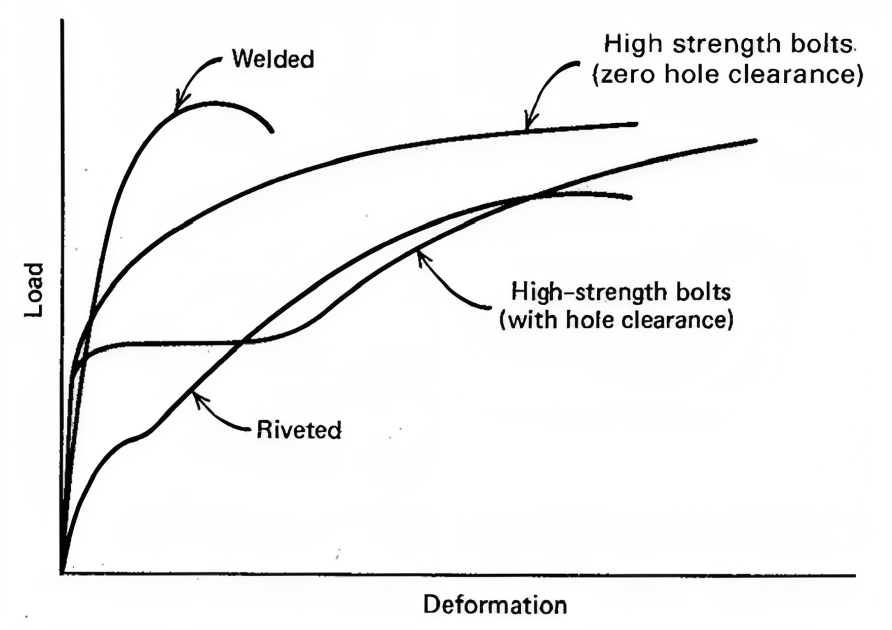
\includegraphics[width=0.75\linewidth]{imgs//ch2/hsbrive-1969.png}
    \caption{Load versus deformation relationships for different fastening methods \cite{steinhardt1969-hybrid}}
    \label{fig-hsbriv-stei}
\end{figure}


One limitation of high-strength bolted connections is their decreased deformation capacity. Welded connections do not experience slip, and the initial stiffness of the joint remains relatively constant until the ultimate load is reached. Based on the load-deformation relationships observed in typical fasteners, it can be inferred that the most suitable combination of fasteners is one that possesses compatible deformation characteristics. In this regard, the preferred combinations seem to be welds in conjunction with slip-resistant high-strength bolts, as well as rivets alongside bolts.

Given that the joint strength of short combination joints is a sum of the strengths of individual fasteners, the specific arrangement of these fasteners within the combination joint becomes inconsequential. Consequently, both the outermost rivets and the rivets within the joint can be interchanged with high-strength bolts, as either arrangement results in a similar ultimate load. However, it should be noted that the location of fasteners does influence the joint strength, as observed in long riveted and bolted joints. In the case of long joints, the replacement of outermost rivets with high-strength bolts proves more effective in enhancing joint strength than replacing the same number of interior fasteners, primarily due to the phenomenon of "unbuttoning." The location of the bolts as well as the rivets configuration will be studied and explored as part of the research objectives of this study.

\subsubsection{Fatigue strength}

The research findings \cite{steinhardt1969-hybrid, reemsnyder1975Fatigue} demonstrated that substituting rivets with preloaded high-strength bolts in areas where cracking was observed or anticipated resulted in a fatigue life improvement ranging from two to six times. It is imperative to ensure the careful extraction of the rivets to be replaced and the accurate installation of the replacement bolts during the rehabilitation process to prevent the introduction of new mechanical flaws, such as burrs, nicks, and gouges. Furthermore, the tests indicated that if cracking is mitigated in the crucial region through rivet replacement, other less highly stressed areas may then become susceptible to becoming critical.


\subsection{HSBs with Weld} \label{sec-hsbweld}

Adding Welds to Mechanically Fastened Joints Welded connections are rigid. Welded connections are stiff. Unlike snug-tightened bolted joints that may slip as they are loaded, welds are not expected to stretch and distribute the applied load to any great extent. In most cases, welds and bearing-type mechanical fasteners will not deform equally.

When welds and mechanical fasteners are used together, load is transferred through the stiffer part; therefore, the weld can carry almost all the load, sharing little with the bolts. That is why caution needs to be taken when welds, bolts, and rivets are combined.Code Provisions. The issue of mixing mechanical fasteners and welds is addressed in AWS D1. 1:2000 Structural Welding Code—Steel \cite{aws2000AWS}. Provision 2.6.3 states that for rivets or bolts used in bearing-type connections (that is, when the bolt or rivet acts as a pin), the mechanical fasteners should not be considered as sharing the load in combination with welds. If welds are used, they should be provided to carry the entire load in the connection. However, connections that are welded to one member and riveted or bolted to another are permitted.


Holtz and Kulak (1970) \cite{holtz1970high} carried out a series of tests on combination joints. In these experiments, a double lap joint featuring both bolts and welds in the same shear plane was subjected to tension loading. They found that bolts carry only a limited amount of load at service loads (considered to be around 1/3 of ultimate load). They also observed that it is unreliable to predict the impact of friction when using pretensioned bolts. Moreover, bolts do not perform efficiently when combined with transverse welds due to the latter's limited ductility.


\subsection{Summarize for the issue of hybrid joint}

During the reconstruction projects following the Second World War, the combined use of diverse connection methods with varying principles presented challenges. For instance, when reinforcing aging riveted structures by welding or partially replacing them with HSB, difficulties arose. Joining components with combined different load transfer mechanism connection methods results in a non-stationary structure, making it difficult to accurately calculate the sharing of loads in the past. As a result, only one of the two types was considered valid for design purposes at the time, denying the cooperative actions expected from their combined use.

The maintenance and repair of ageing riveted bridges is expected to face increasing challenges from now on. Bridges must achieve a compromise between suitable flexibility and rigidity. The addition of reinforcing elements to a completed bridge may upset this equilibrium and create problems. Consequently, post-construction reinforcement of a bridge may present a challenge by using hybrid connection.

In addition, for new structural components, the rational use of hybrid joints can effectively improve the strength of the joints and shorten the length of the joints as much as possible, while meeting the required strength to make the joint compact.  However, unlike the reinforcement of an existing structural component, new structural components raise issues of structural stability, durability and strict requirements for allowable deformation, and require a series of tests before they can be installed.

In summary, this work focuses on the following technical issues:

\begin{itemize}
    \item The primary technical challenge lies in the lack of understanding regarding the load transfer mechanism when combining connections with different mechanical principles.
    \item To use hybrid joints effectively, it is essential to comprehend not only how the load gets transferred but also the optimal arrangement of fasteners. Different arrangements may produce different load transfer effects, so exploring the reasonable fastener arrangement scheme will be an important technical problem.
    \item The stiffness of Friction connection and bearing connection are different. In the case of a friction connection, there will be a small elastic dislocation (slip) before occurrence, which is a different mechanical mechanism from the elastic deformation of a bearing connection. Exploring the deformation capacity of the bearing and friction combination is also an important technical subject.
    \item After understanding the load transfer mechanism, strength and deformation performance of hybrid connections, it is necessary to define their limit states and to devise how to differentiate between the limit states and their corresponding strength equations.
    
\end{itemize}

%https://www.thefabricator.com/thefabricator/article/arcwelding/mixing-welds--bolts
%https://pressbooks.bccampus.ca/powr4406/chapter/bolted-and-welded-joints/

%\subsection{IFB-HSB}




% \section{Regulations and standards}

% \subsection{Riveted joint}

% Shear resistance, per shear plane, Eurocode:
% \begin{equation}
% F_{\mathrm{v}, \mathrm{Rd}}=\frac{0,6 f_{\mathrm{ur}} A_0}{\gamma_{\mathrm{M} 2}}
% \end{equation}
\chapter{Experiment of Rivet-HSB hybrid Connection}
\label{ch4}

%%%%%%%%%%%%%%%%%%%%%%%%%%%%%%%%%%%%%%%
% IMPORTANT
\begin{spacing}{1.25} %THESE FOUR
\minitoc % LINES MUST APPEAR IN
\end{spacing} % EVERY
\onehalfspacing % CHAPTER
% COPY THEM IN ANY NEW CHAPTER
%%%%%%%%%%%%%%%%%%%%%%%%%%%%%%%%%%%%%%%

\section{Slip coefficient of riveted joint}

\subsection{background}

Rivets were widely used in the world to fasten steel members in the early days, and also used for cross-section connections for steel bridges. Since 1950, countries worldwide have been issued design specifications for high-strength bolts connection, and high-strength bolts connection have gradually replaced rivet connections. However, many riveted bridges are still in service \cite{Collette2014Experimental1880s1890s}. Some of the rivets might be corroded and loosen due to deterioration of the paint coating. The reduction of the volume of a rivet's head is severely affected fatigue life \cite{Heinemeyer2011TheConnections}. Studies have also pointed out the influence of rivets' material loss on these bridge structure elements' remaining bearing capacity \cite{Hashimoto2010,Macho2016}. For structural performance recovery or to extend their service life, the riveted bridges have to repair or reinforce by replacing the corroded rivets with high-strength bolts. Replacing the rivets with a high-strength bolt for changing to the frictional joint is a desirable approach to repairing the corroded riveted joint \cite{KOMATSU2015}. 
    
Applying such repair, whether it satisfies the frictional joints' performance requirements depends on the slip coefficient. However, the riveted joint surface's slip coefficient with red lead paint for corrosion is not specified. Therefore, giving a proper evaluation of the slip coefficient is one of the purposes of this paper.
Lead is an excellent anti-corrosive, lead-based paint that could be well protecting a steel structure from the element. Especially red lead (Pb3O4) was once widely used for bridges anti-corrosion paint. However, Lead-based paint has been a significant cause of lead poisoning. Countries around the world are beginning to call for an end to the use of Lead-based paint. The U.S. Consumer Product Safety Commission (CPSC) has already started banning lead-based paint in 1977 \cite{CPSC1977}. In 1987, Japan completely stopped using red lead as anti-corrosion paints for steel structures \cite{rtri1987Steel}. So far, the use of red lead has been completely discontinued and replaced by inorganic resin coatings. Red lead and rivets are used on steel bridges almost in the same period. Since rivets are designed to transmit load by shearing force, the friction performance of riveted joint surfaces with red lead paint is unspecified. 
In this study, the authors have got the opportunity to obtain a 90-year-old riveted bridge's cross-beam. The joint part was cut out from this bridge's cross-beam and evaluated the riveted joint surface's aging condition in natural corrosion weakening by microscope observation and elemental analysis. In addition, the slip test is conducted to investigate the joint surface's slip coefficient of the riveted joints experimentally. Finally, the pressure distribution test is conducted using a pressure measurement film to explore the pressure distribution and the effective contact pressure area of riveted joints' surface.


\subsection{Joint faying surface's aging condition}

The bridge of the research object has been in use for 90 years. The bridge's paint was probably damaged, and the joint surface was probably corroded due to aging. In order to investigate the condition of the aging bridge joint's surface, 40mm x 40mm compact specimens cut out from the joint to conduct microscope observation, Fourier-transform infrared spectroscopy analysis (FT-IR), and Energy Dispersive X-ray Spectroscopy (EDX) analysis.

\subsubsection{Microscope observation} \label{ch3sec2-1}

Depending on where the specimen was taken out, the red lead's aging condition has been found different. The research has shown that the red lead paint adjacent to the rivet hole has been compromised due to high temperature and clamping force by riveting. The friction coefficient may be affected by this \cite{Leonetti2020RivetBridges}.

The red lead on the joint surface has partly peeled off, and the black oxide of the steel can be observed, which indicates that the red lead's adhesion has become poor over aging, as shown in Fig. \ref{ch3fig2b}

\begin{figure}
    \centering
    \begin{subfigure}[t]{0.4\textwidth}
    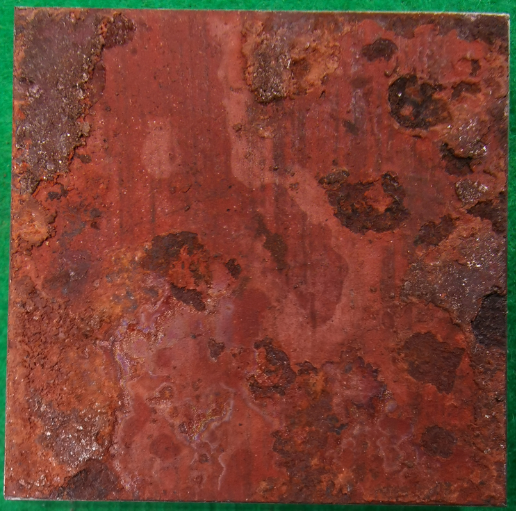
\includegraphics[width=\linewidth]{imgs/ch3/fig2a.png}
    \caption{Normally}
    \label{ch3fig2a}  
    \end{subfigure}
    \hfill
    \begin{subfigure}[t]{0.4\textwidth}
    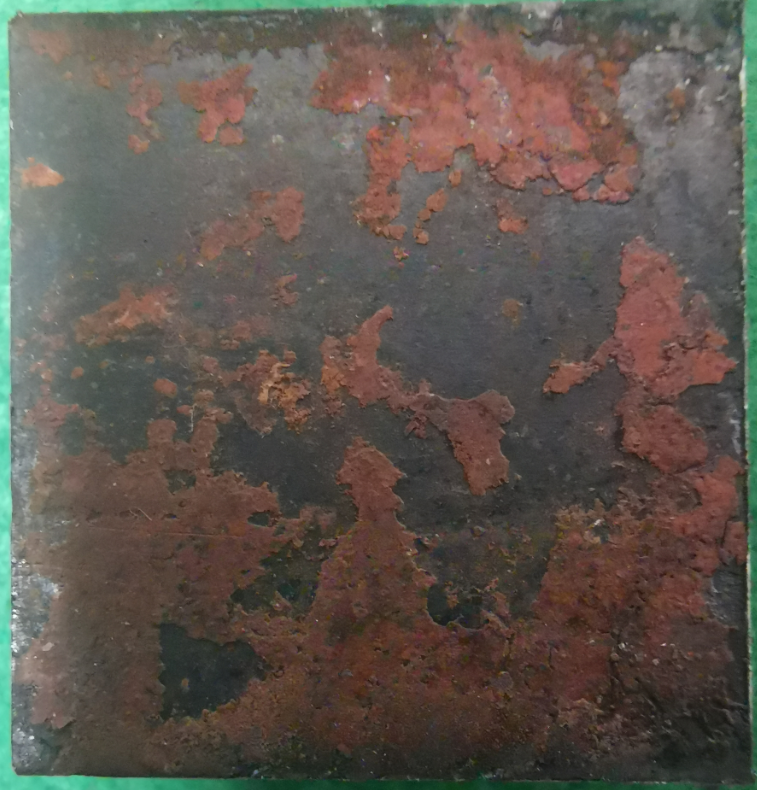
\includegraphics[width=\linewidth]{imgs/ch3/fig2b.png}
    \caption{Seriously}
    \label{ch3fig2b}  
    \end{subfigure}
    \caption{Faying surface for riveted joint}
\end{figure}

As shown in Fig. \ref{ch3fig3}, the joint surface was observed with an electron microscope of 50 times and 600 times. The orange-red substance is red lead, and the black primer is the black oxide of steel. No obvious traces of rust are found on the joint surface. The light reflecting material in the picture is a resin coating, and it will be confirmed by elemental analysis for the next section.

\begin{figure}
    \centering
    \begin{subfigure}[t]{0.4\textwidth}
    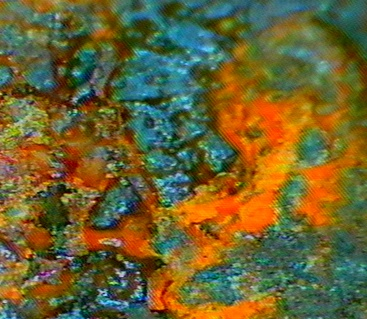
\includegraphics[width=\linewidth]{imgs/ch3/fig3a.jpeg}
    \caption{50X}
    \label{ch3fig3a}  
    \end{subfigure}
    \hfill
    \begin{subfigure}[t]{0.4\textwidth}
    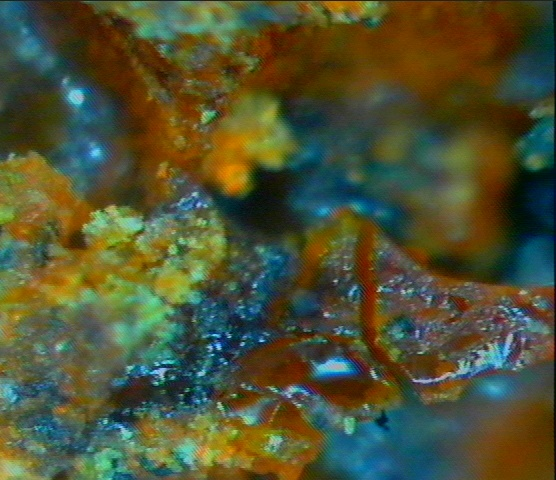
\includegraphics[width=\linewidth]{imgs/ch3/fig3b.jpeg}
    \caption{600X}
    \label{ch3fig3b}  
    \end{subfigure}
    \caption{Microscope observation}
    \label{ch3fig3}
\end{figure}

\subsubsection{FT-IR and EDX analysis}

This study randomly selected three specimens from different positions of the joint and conducted FT-IR analysis on the joint surface. Furthermore, the presence of elements on the joint surface detected by EDX analysis. FT-IR spectra of the joint surface are illustrated in Fig. \ref{ch3fig4}. The spectrum consists of many sharp and weak bands in the region of 700–900 cm-1, in addition to a few bands in the region of 1,500–2,000 cm-1. Most of the main peaks corresponding to vinyl acetate (C4H6O2) were detected \cite{baskaran2004Vibrational}, but no main peaks corresponding to Iron (III) oxide (Fe2O3) were found. The study has shown that incorporating various metallic additives into polymer matrices can produce polymer-matrix composites and improve their properties for specific applications \cite{dong2006Polyvinylbutyral}. In order to enhance the adhesion of red lead, a resin-based primer is usually applied before the red lead. It can be considered that the vinyl acetate detected by FT-IR acts as a resin-based primer to enhance the adhesion of red lead.

\begin{figure}
    \centering
    \begin{minipage}[t]{0.7\textwidth}
    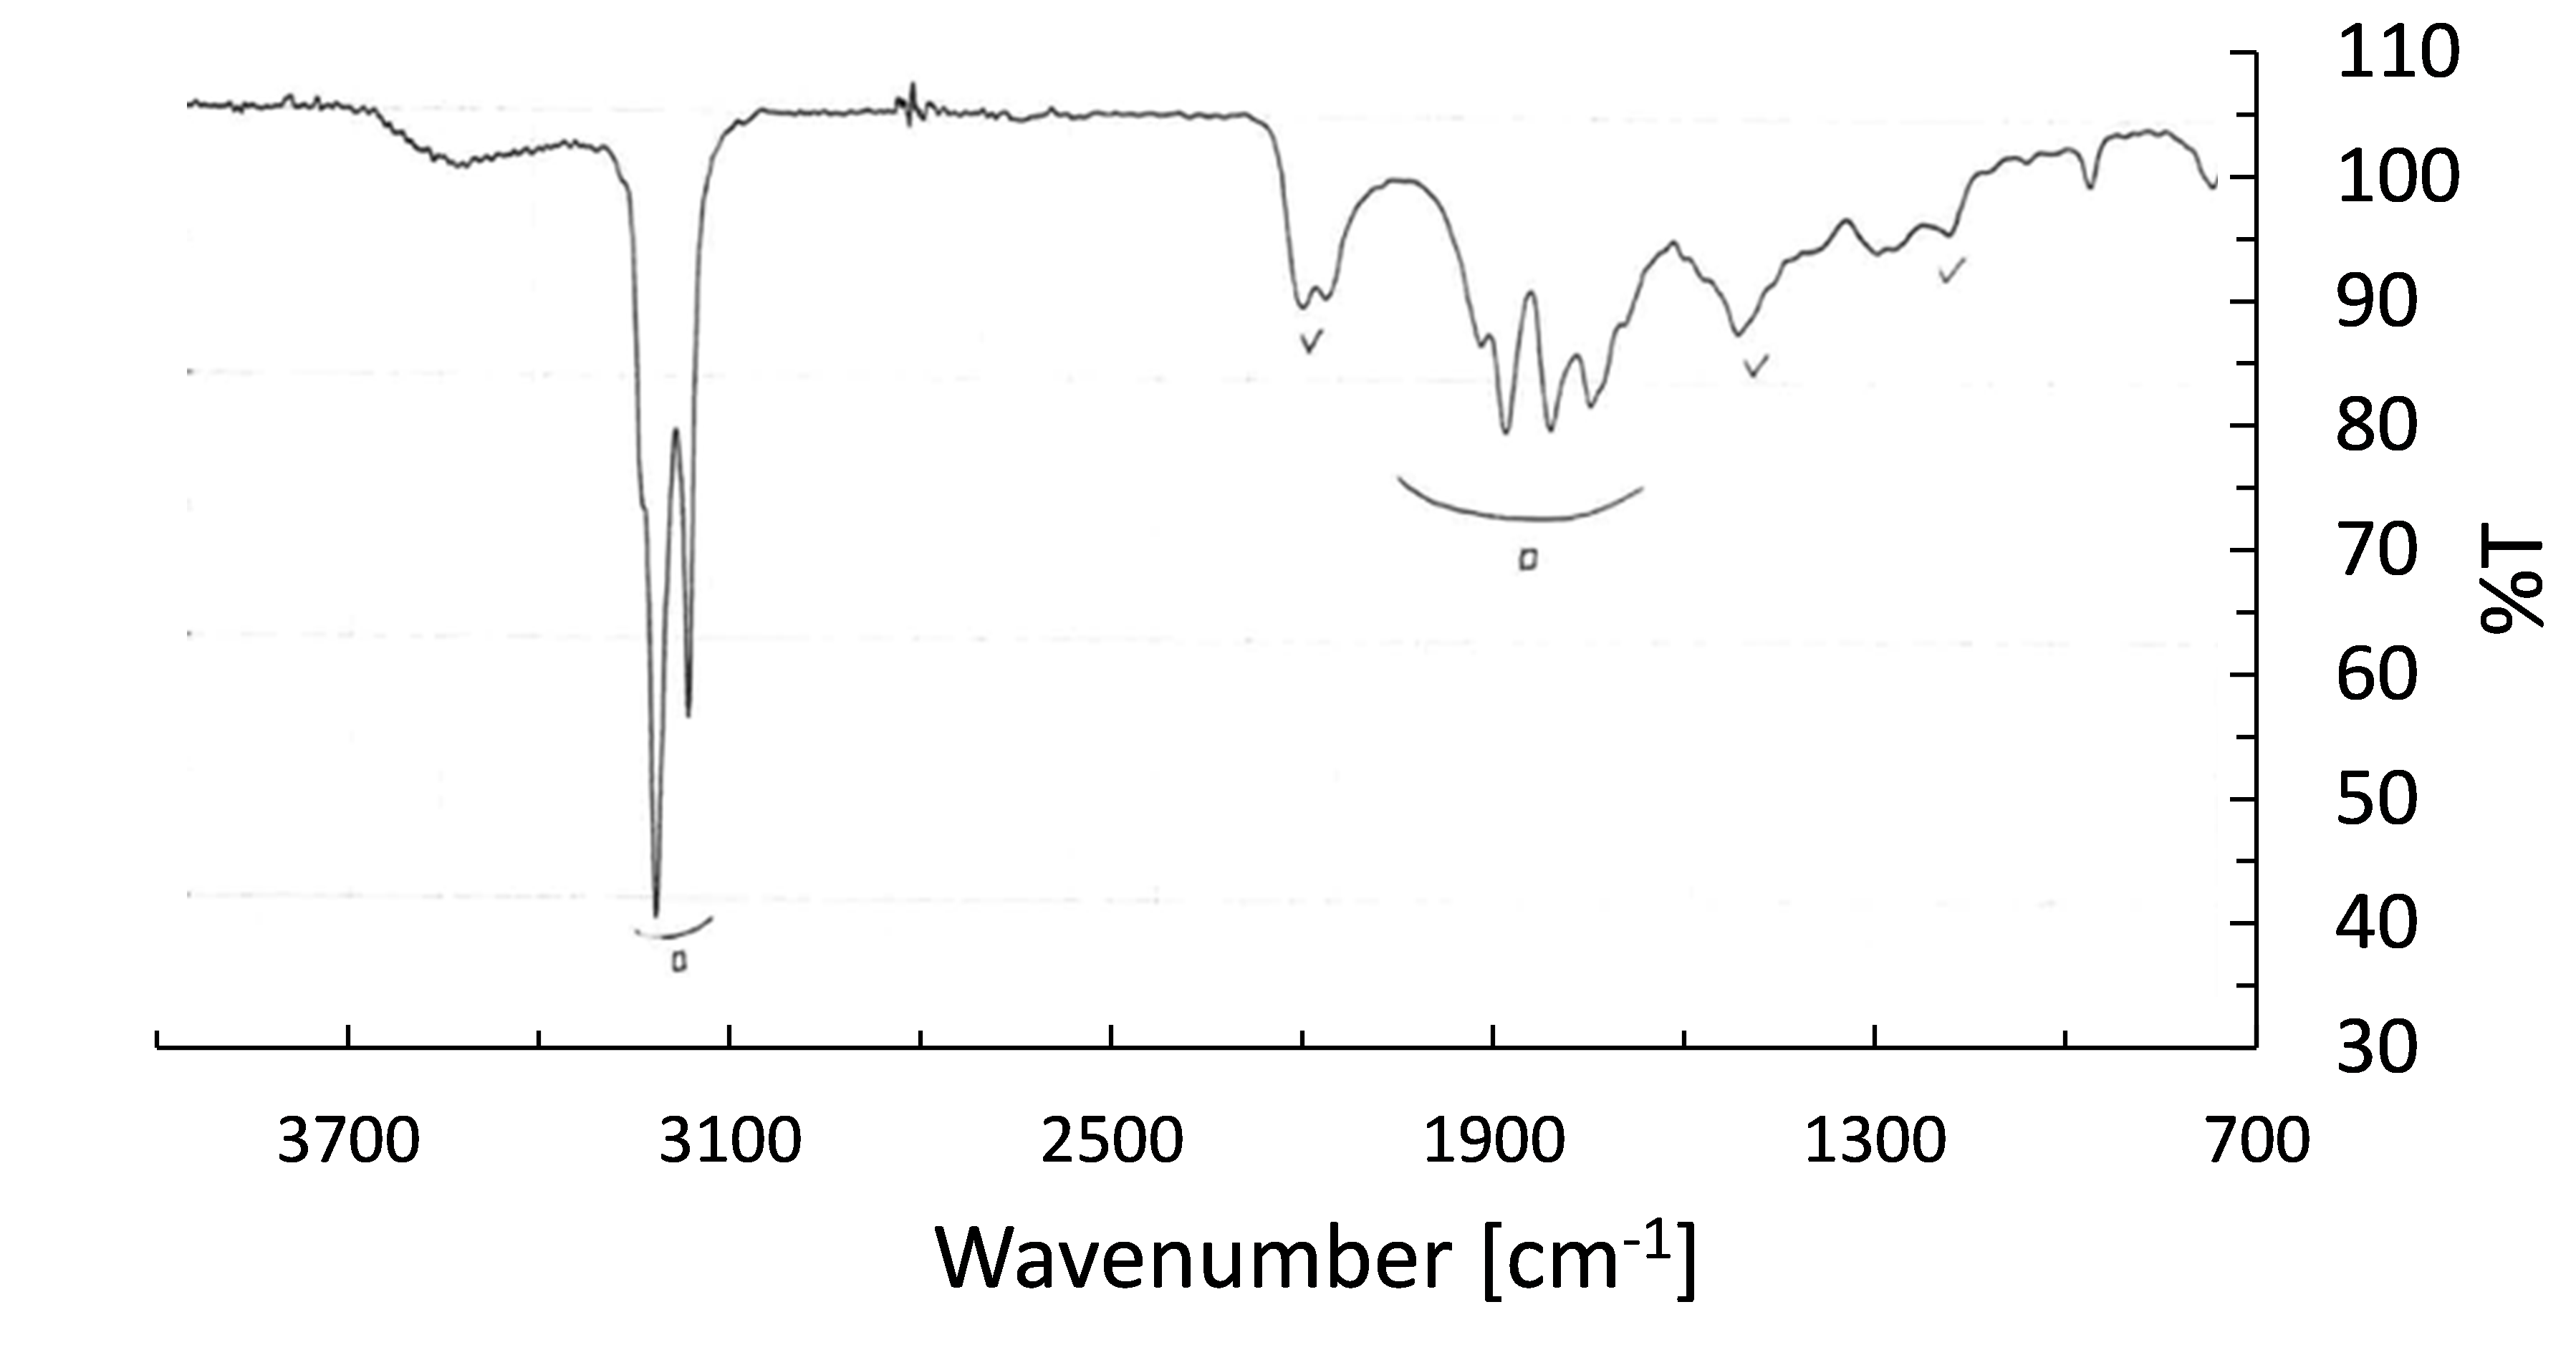
\includegraphics[width=\linewidth]{imgs/ch3/fig4.png}
    \caption{FT-IR spectra of the joint surface}
    \label{ch3fig4}  
    \end{minipage}
    \begin{minipage}[t]{0.7\textwidth}
    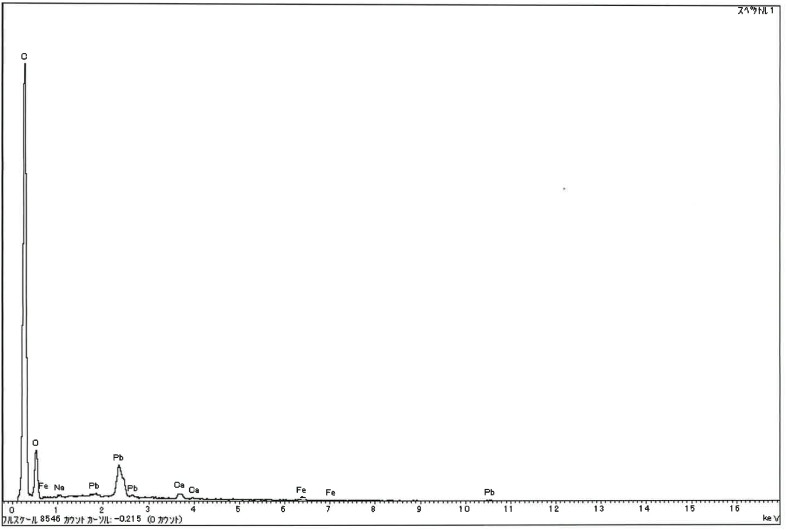
\includegraphics[width=\linewidth]{imgs/ch3/fig5.png}
    \caption{EDX-spectrum of the joint surface}
    \label{ch3fig5}  
    \end{minipage}
\end{figure}

From Fig. \ref{ch3fig5}, it can be inferred that the lead oxide on the joint surface was confirmed to exist on the joint surface, and there was also iron oxide. By means of FT-IR spectra that can confirm iron oxide is not red rust(iron(III) oxide), but a black oxide film formed when the steel is manufactured.


\subsection{Compact slip test}

\subsubsection{Loading and measuring methods}

Fig. \ref{ch3fig6} shows a loading machine and loading methodology, and Fig. \ref{ch3fig6a}, Fig. \ref{ch3fig6b} shows the general diagram and the detailed diagram, respectively. A screw-jack applies a horizontal load to two sets of specimens until it reaches the target clamping force. And they are then applying a vertical load to the specimens by a universal loading machine. There is a Displacement Transducer on each side of specimens, and they will be initialed to monitor the slip of the test specimen after the horizontal load is complete. Both horizontal and vertical loads applied were monitored by using a load cell.

\begin{figure}
    \centering
    \begin{subfigure}[t]{0.58\textwidth}
    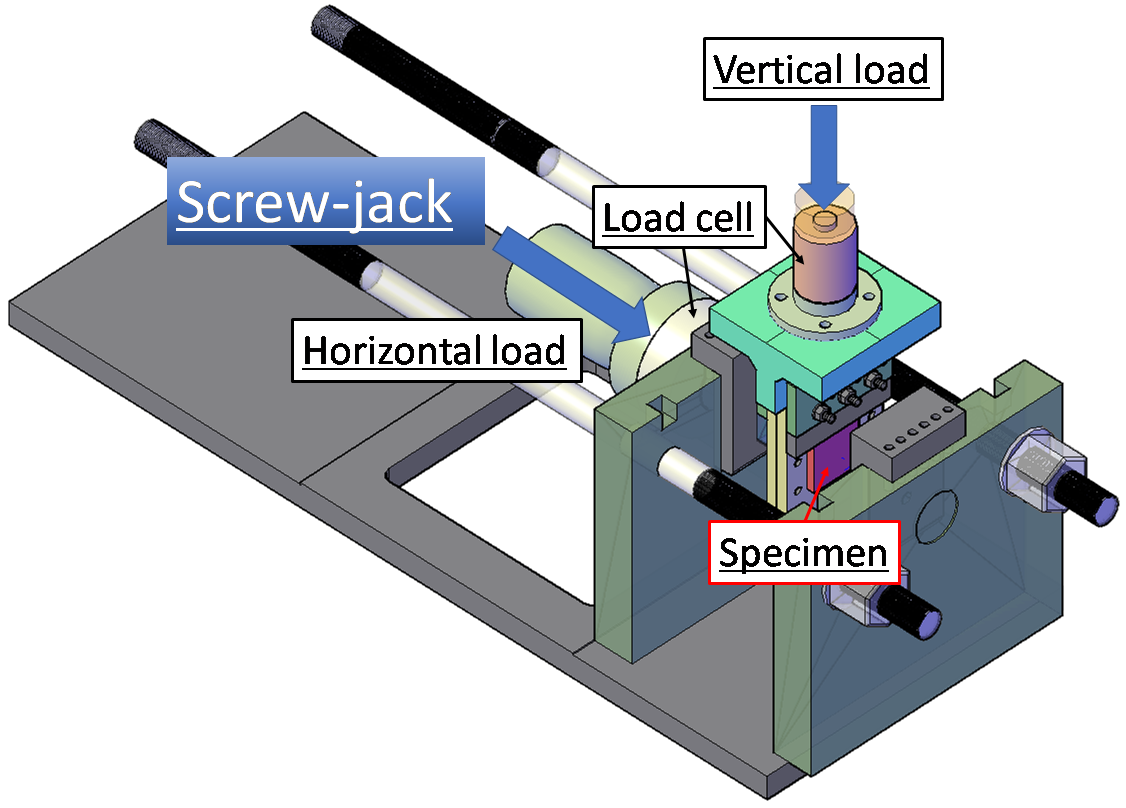
\includegraphics[width=\linewidth]{imgs/ch3/fig6a.png}
    \caption{General diagram}
    \label{ch3fig6a}  
    \end{subfigure}
    \hfill
    \begin{subfigure}[t]{0.38\textwidth}
    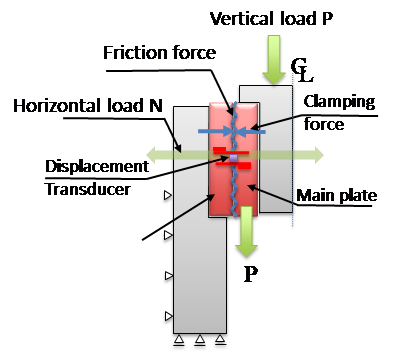
\includegraphics[width=\linewidth]{imgs/ch3/fig6b.png}
    \caption{Detailed diagram}
    \label{ch3fig6b}  
    \end{subfigure}
    \caption{Test setup}
    \label{ch3fig6}
\end{figure}

The universal loading machine will be loading on 0.5 kN/s until a slip occurred. Then, the slip coefficient is calculated by the relationship between the vertical load and displacement.

\subsubsection{Specimens}

A total of 48 set specimens are cut out from the same riveted bridge's joint. The position of cut out and the size of specimens as shown in Figure 7a, and b respectively. In order to explore the influence of the clamping force on the slip coefficient, the specimens are divided into three groups according to the different clamping forces introduced. The three groups of specimens are 24 sets of 100\% standard clamping forces, 12 sets of 75\%, and 50\% standard clamping forces $N$. 

\begin{figure}
    \centering
    \begin{subfigure}[t]{0.48\textwidth}
    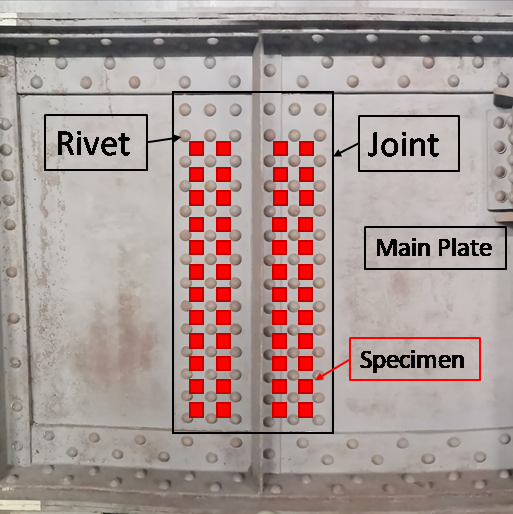
\includegraphics[width=\linewidth]{imgs/ch3/fig7a.png}
    \caption{Cross-beam}
    \label{ch3fig7a}  
    \end{subfigure}
    \hfill
    \begin{subfigure}[t]{0.48\textwidth}
    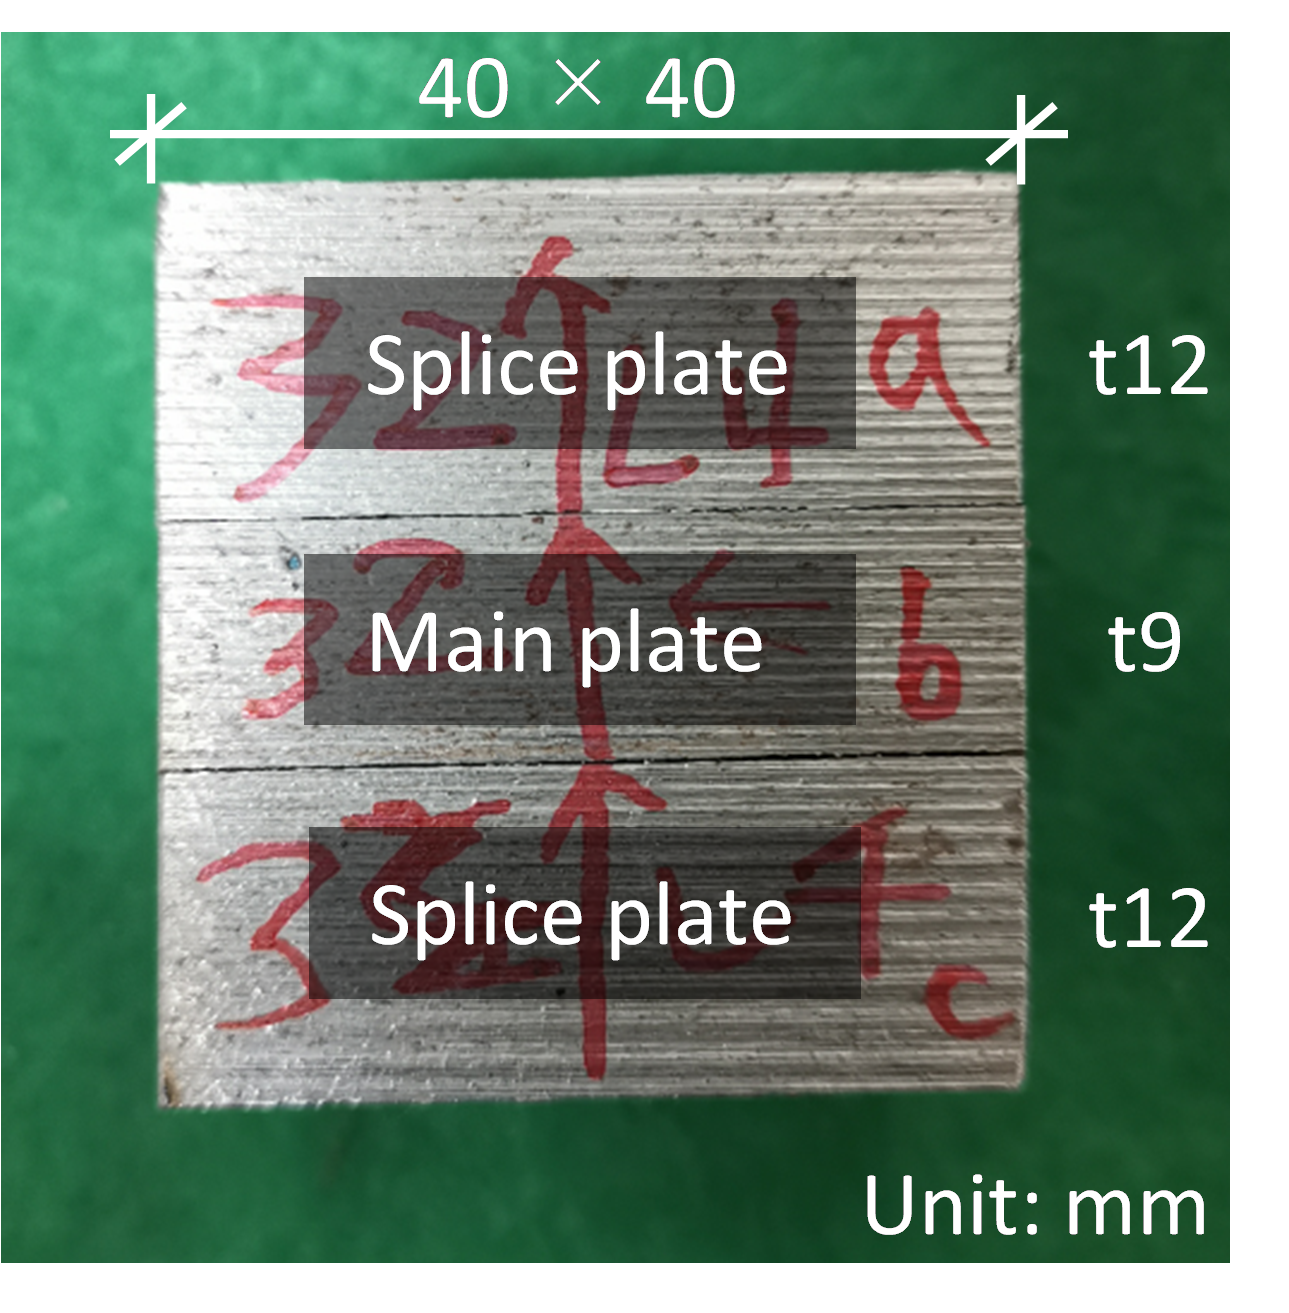
\includegraphics[width=\linewidth]{imgs/ch3/fig7b.png}
    \caption{Specimens section}
    \label{ch3fig7b}  
    \end{subfigure}
    \caption{Specimens' cut out location and size}
\end{figure}

The standard clamping force is calculated by multiplying the standard bolt contact pressure by the contact area. The assumed contact pressure area was calculated as the contact pressure distributed at 45° \cite{rotscher1927maschinenelemente}, as shown in Fig. \ref{ch3fig8}. When the splice plate's thickness is 12 mm, the standard bolt contact pressure can be calculated as 64.9 N/mm2. Here it is assumed that the bolt is the most commonly used F10T-M22 in Japanese bridges.


\begin{figure}
\centering
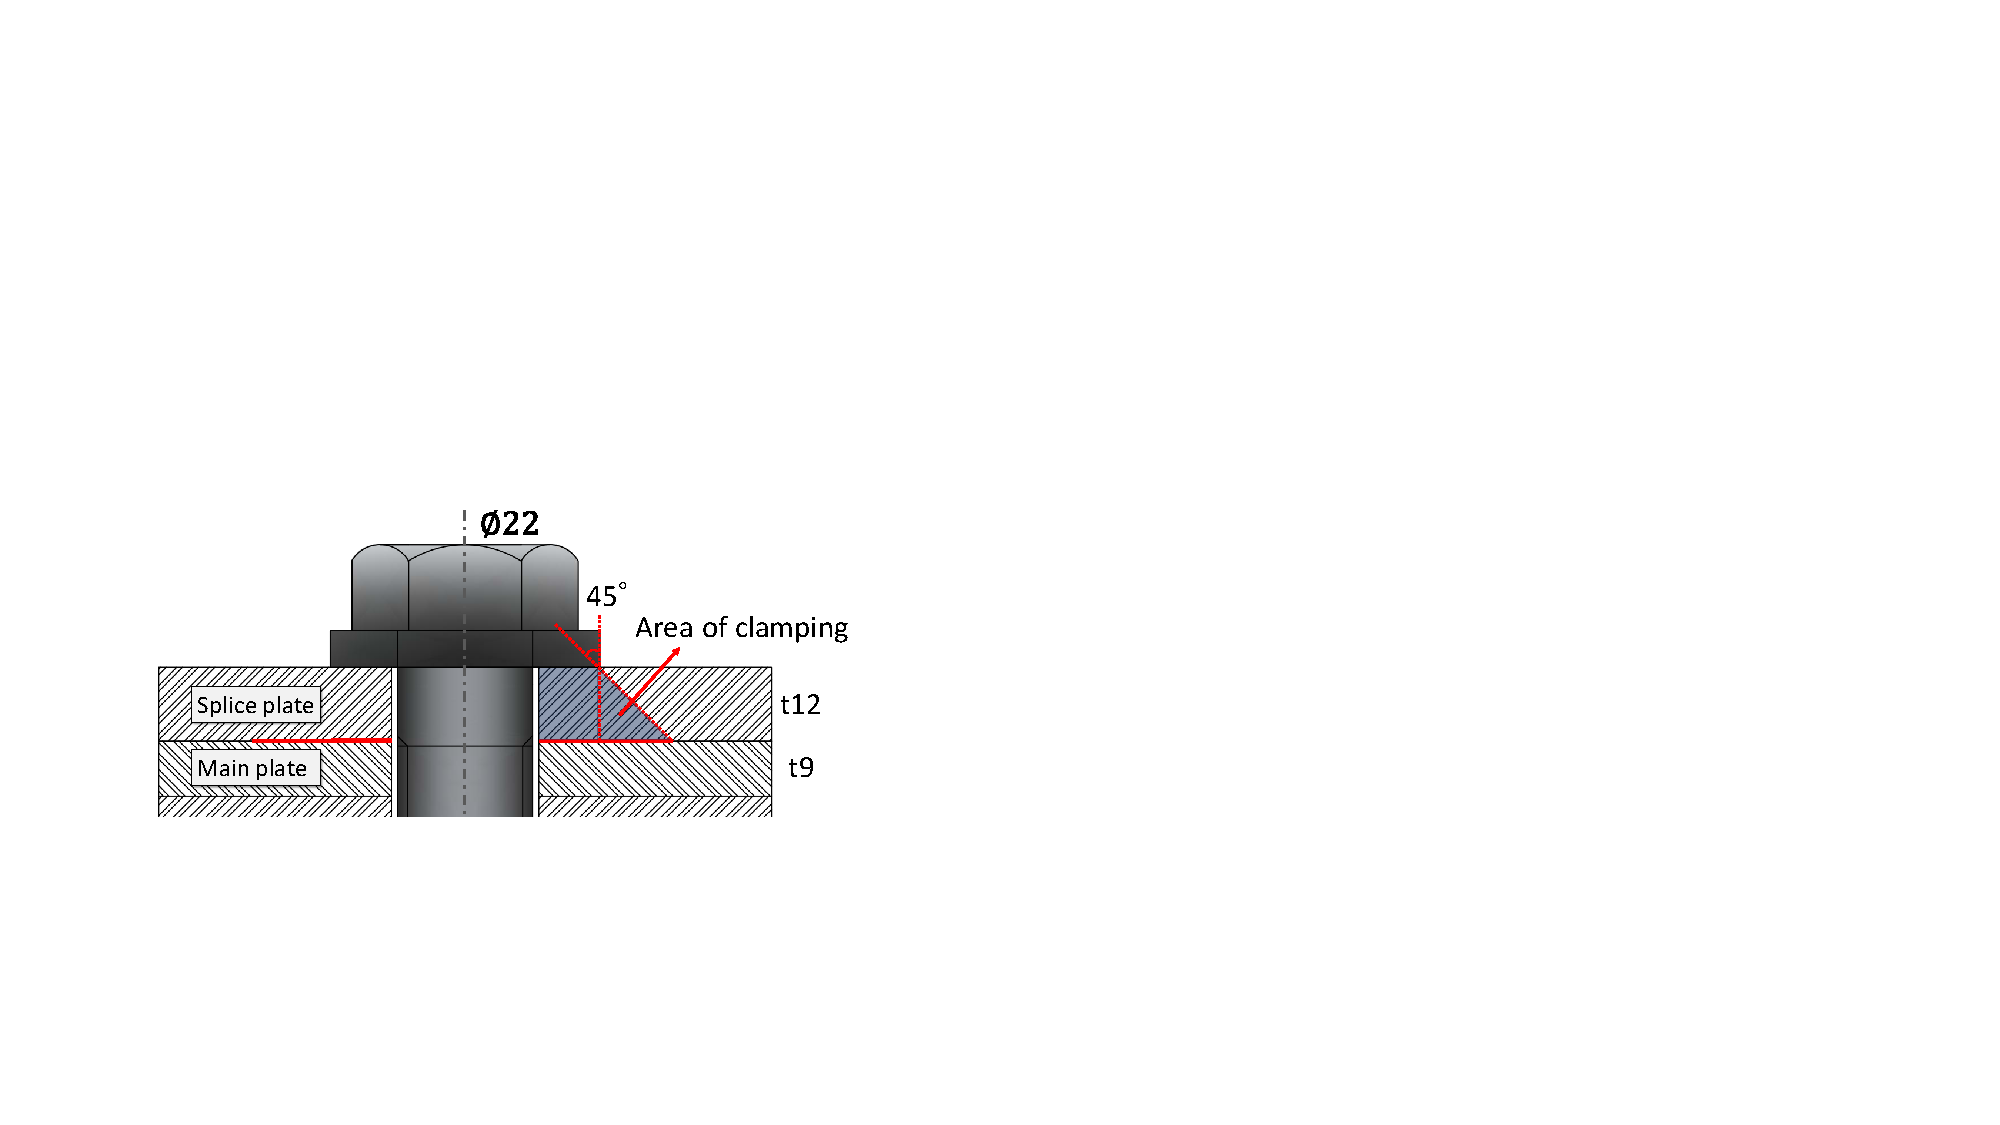
\includegraphics[width=0.65\linewidth]{imgs/ch3/fig8.pdf}
\caption{Definition of clamping area (unit: mm)}
\label{ch3fig8}  
\end{figure}

For example, for the M22 size bolt, the euivalent contact area $A_{ct-m22}$ is:
\begin{equation*}
    A_{ct-m22} = \pi (r_h-r_b)^2
\end{equation*}

Where, the  bolt shank radius $r_b$ is 11 mm, bolt hole radius $r_h$ is 11.75 mm.
the equivalent contact pressure $\sigma_{ct-m22}$ is:
\begin{equation*}
    \sigma_{ct-m22} = \frac{N}{A_{M22}} = 64.9 Mpa
\end{equation*}

Where, $N$ is the bolt standard preload, M22-F10T bolt is 205 kN.
The applied horizontal force (Converted preload) $N_{cp}$ is 
\begin{equation*}
    N_{cp} = \sigma_{ct-m22} \times A_{cts} =64.9 \times 40 \times 40 = 103.8 kN
\end{equation*}
Where, $A_{cts}$ is specimens size for compact slip test


\subsubsection{Test result}

The test results are summarized in Table \ref{ch3tab1}. The table summarizes the slip coefficients and their variation of all the specimens with 100\%, 75\%, and 50\% of standard clamping force.

\begin{table}[htbp]
\centering
\caption{Summary of the slip coefficient and estimation of variability}
\label{ch3tab1}
\scalebox{0.95}{
\begin{tabular}{@{}cccccccc@{}}
\toprule
\multirow{3}{*}{Specimens} &
  \multicolumn{3}{c}{Slip coefficient} &
  \multirow{3}{*}{\begin{tabular}[c]{@{}c@{}}Standard \\ Deviation \\ (SD, $\sigma$) \end{tabular}} &
  \multirow{3}{*}{\begin{tabular}[c]{@{}c@{}}Standard \\ Error \\ (SE) \end{tabular}} &
  \multirow{3}{*}{\begin{tabular}[c]{@{}c@{}}Coefficient \\ of Variation \\ (C.V.) \end{tabular}} &
  \multirow{3}{*}{\begin{tabular}[c]{@{}c@{}}The \\ Number \\ of data \end{tabular}} \\ \cmidrule(lr){2-4}
        & \multirow{2}{*}{Average} & \multirow{2}{*}{Max}   & \multirow{2}{*}{Min}   &        &        &        &    \\
        &   &     &     &        &        &        &    \\ \midrule
All     & 0.274   & 0.386 & 0.173 & 0.0525 & 0.0076 & 0.1917 & 48 \\
100\%CF & 0.291   & 0.386 & 0.192 & 0.0491 & 0.0100 & 0.1688 & 24 \\
75\%CF  & 0.240   & 0.341 & 0.173 & 0.0482 & 0.0139 & 0.2009 & 12 \\
50\%CF  & 0.274   & 0.351 & 0.208 & 0.0504 & 0.0145 & 0.1839 & 12 \\ \bottomrule
\end{tabular}}
\end{table}

The average slip coefficient is 0.274, the coefficient of variation is 0.19, and the -2σ is 0.169. It can be found that the degree of dispersion of the slip coefficient is not low. Furthermore, it could be concluded that the slip coefficient from the slip test follows a normal distribution by the Shapiro-Wilk normality test \cite{shapiro1965Analysis}. The normal distribution of the slip coefficient is shown in Fig. \ref{ch3fig10}. The 95\% confidence interval is presented as the arithmetic mean ± 1.96 SE (Standard Error) (0.259--0.289).

\begin{figure}
    \centering
    \begin{subfigure}[t]{0.48\textwidth}
    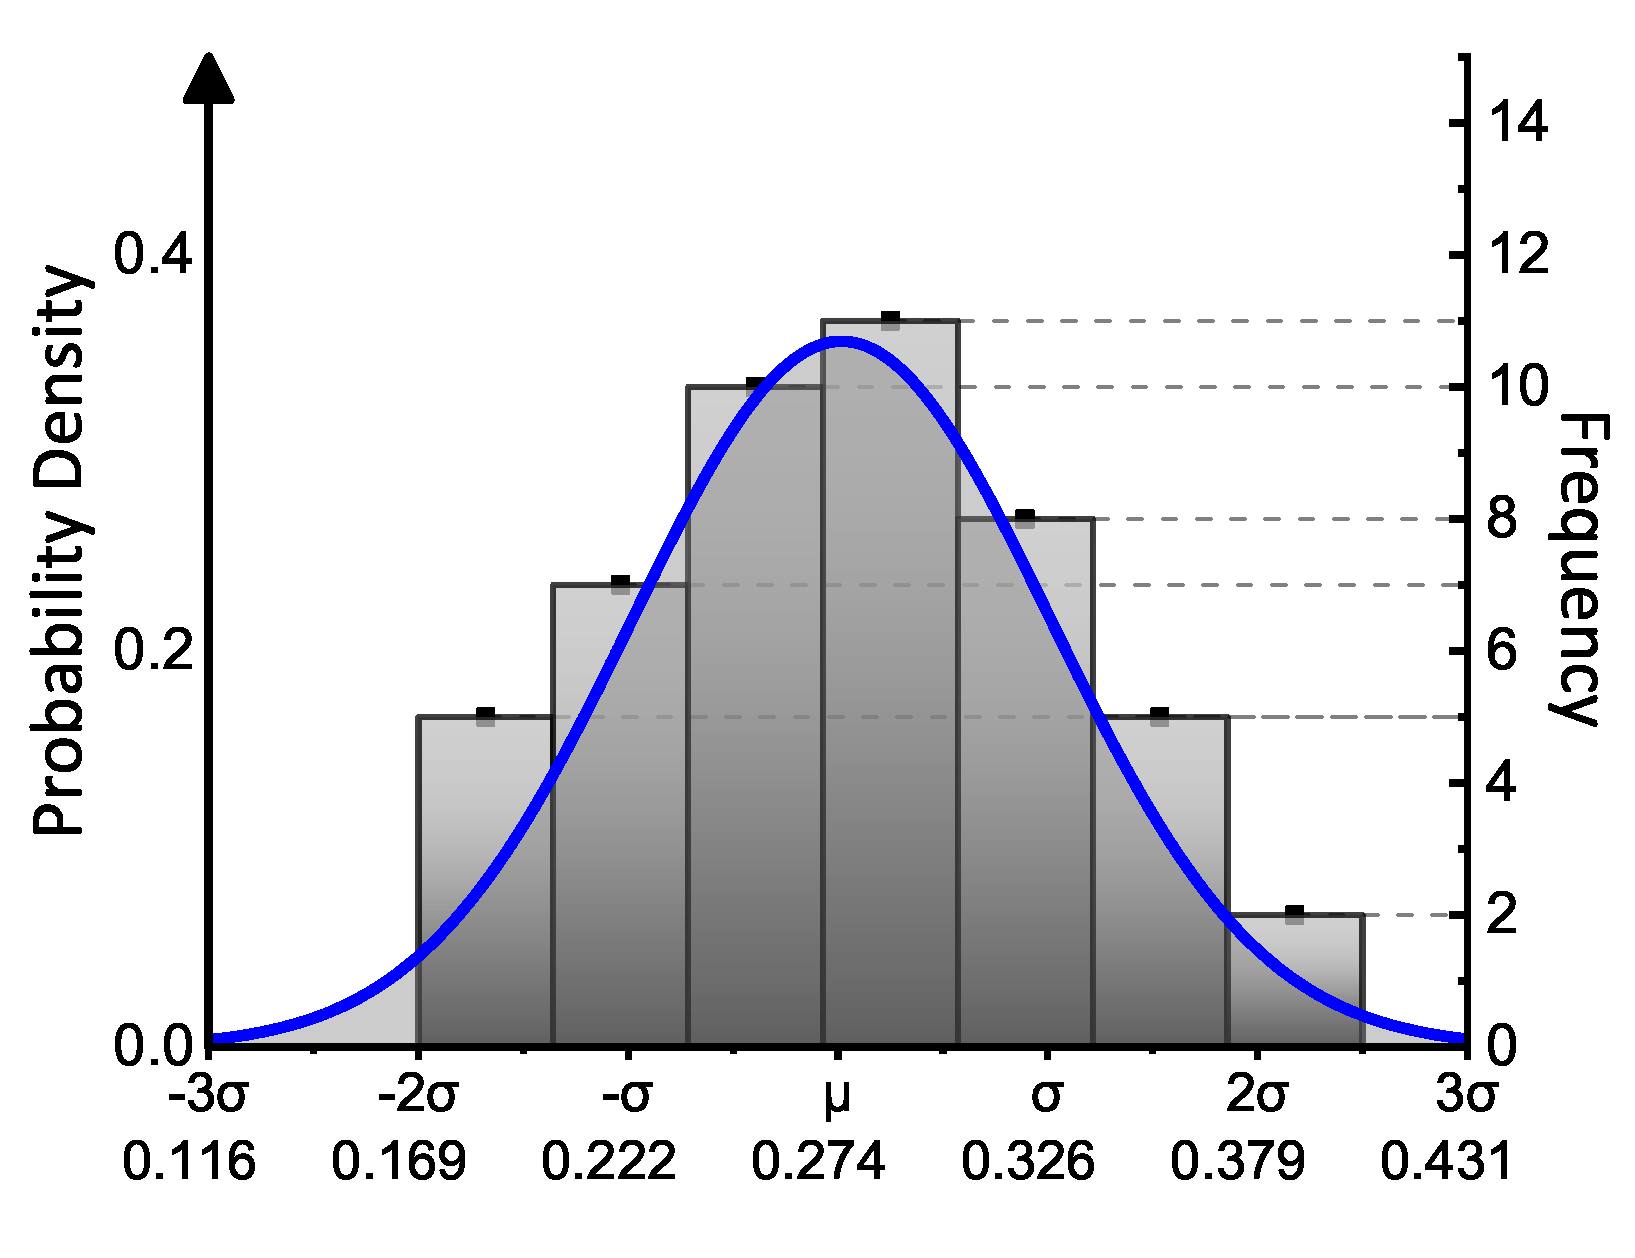
\includegraphics[width=\linewidth]{imgs/ch3/fig10a.eps}
    \caption{Normal distribution}
    \label{ch3fig10a}  
    \end{subfigure}
    \hfill
    \begin{subfigure}[t]{0.48\textwidth}
    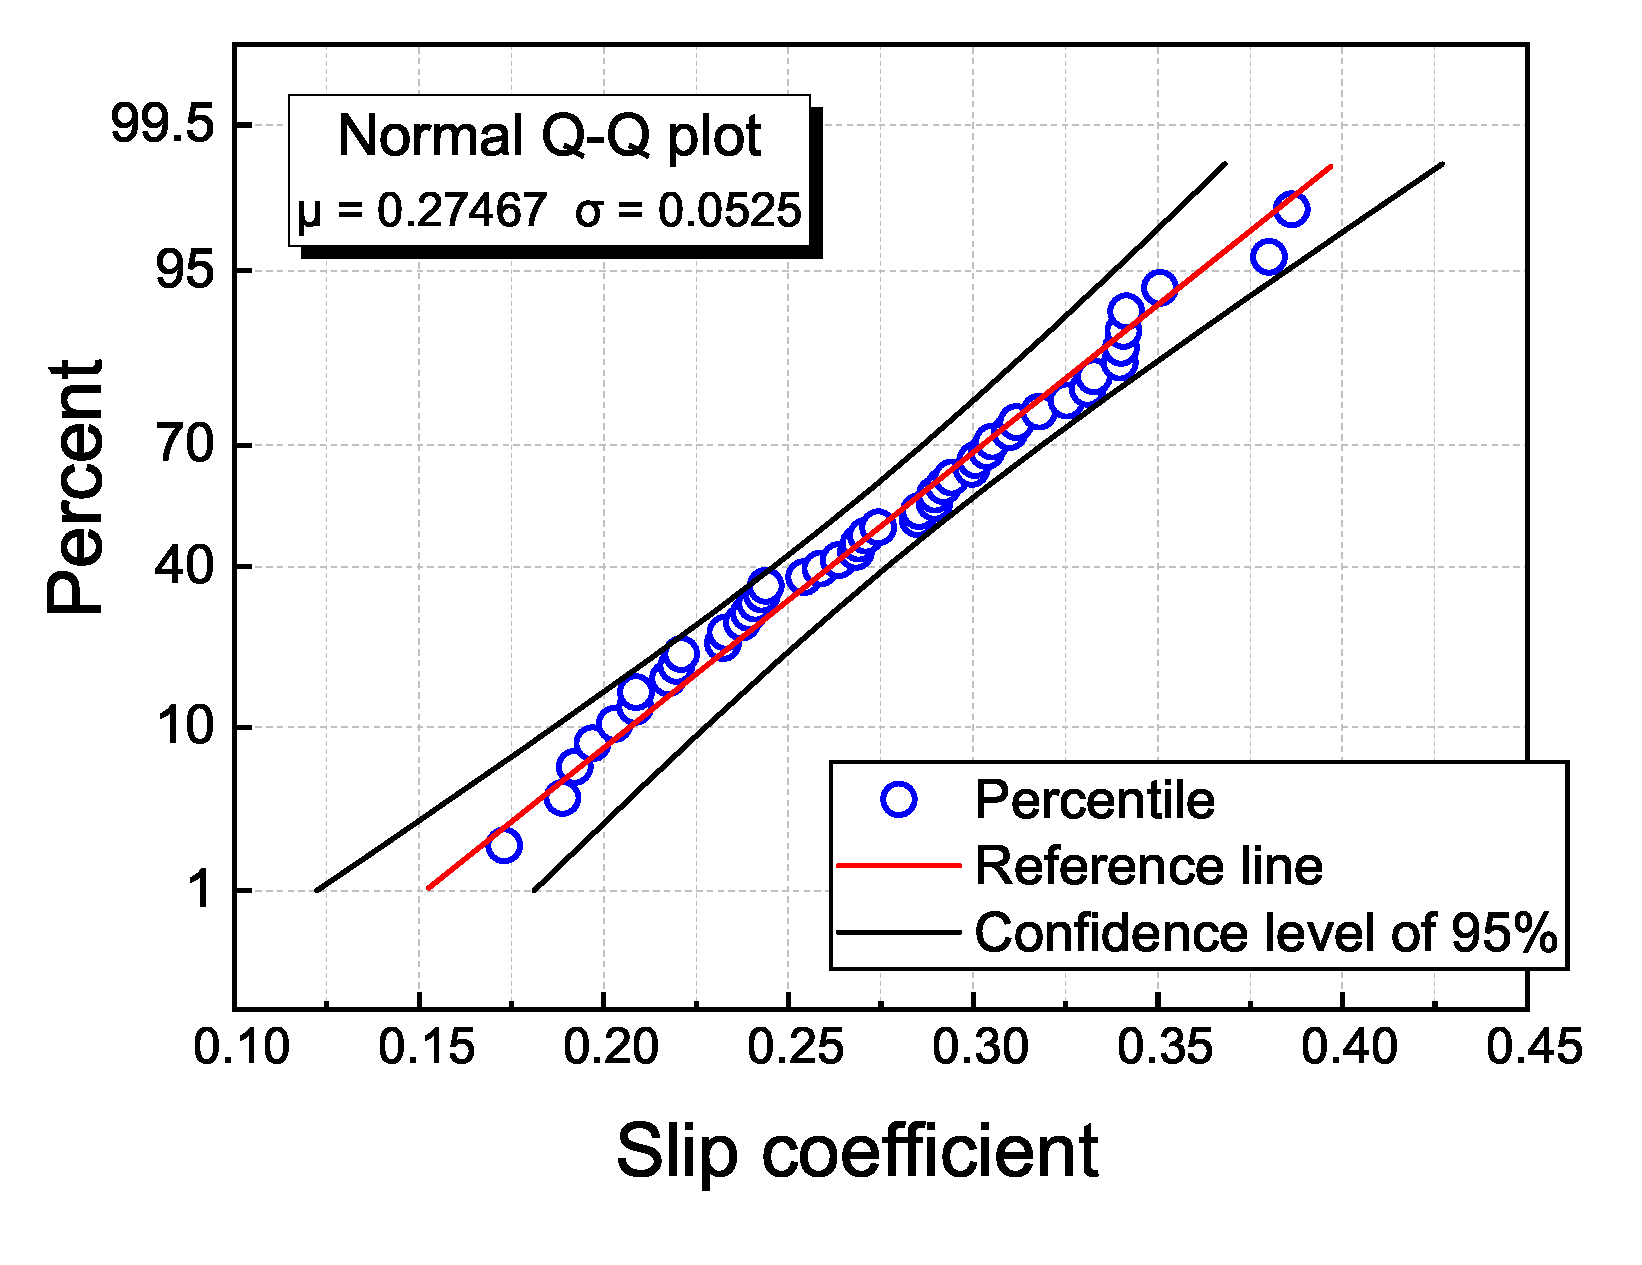
\includegraphics[width=\linewidth]{imgs/ch3/fig10b.eps}
    \caption{Q-Q plot}
    \label{ch3fig10b}  
    \end{subfigure}
    \caption{Slip coefficient distribution}
    \label{ch3fig10} 
\end{figure}

Besides, when the riveted joint surface is red lead paint, replacing the rivet with a high-strength bolt, the expected slip coefficient is 0.25-0.28 by Railway technical research institute in Japan \cite{rtri1992Manual}. However, in this experiment, it can be calculated that there is a 36\% probability that the slip coefficient is below 0.25. 

The specimens' size could cause this, and the red lead distribution is uneven, resulting in a very low slip coefficient accrued in some specimens.

The relationship between the slip coefficient and the clamping force is shown in Fig. \ref{ch3fig11}. It can be observed from the figure that the degree of dispersion of the slip coefficient has no obvious relationship with the change of clamping force; also, it can be calculated that the correlation coefficient between clamping force and slip coefficient is 0.21. On the other hand, the relationship between the slip load and clamping force is shown in Fig. \ref{ch3fig12}. As the clamping force increases, the slip load also increases.

\begin{figure}
\centering
\begin{minipage}[t]{0.48\textwidth}
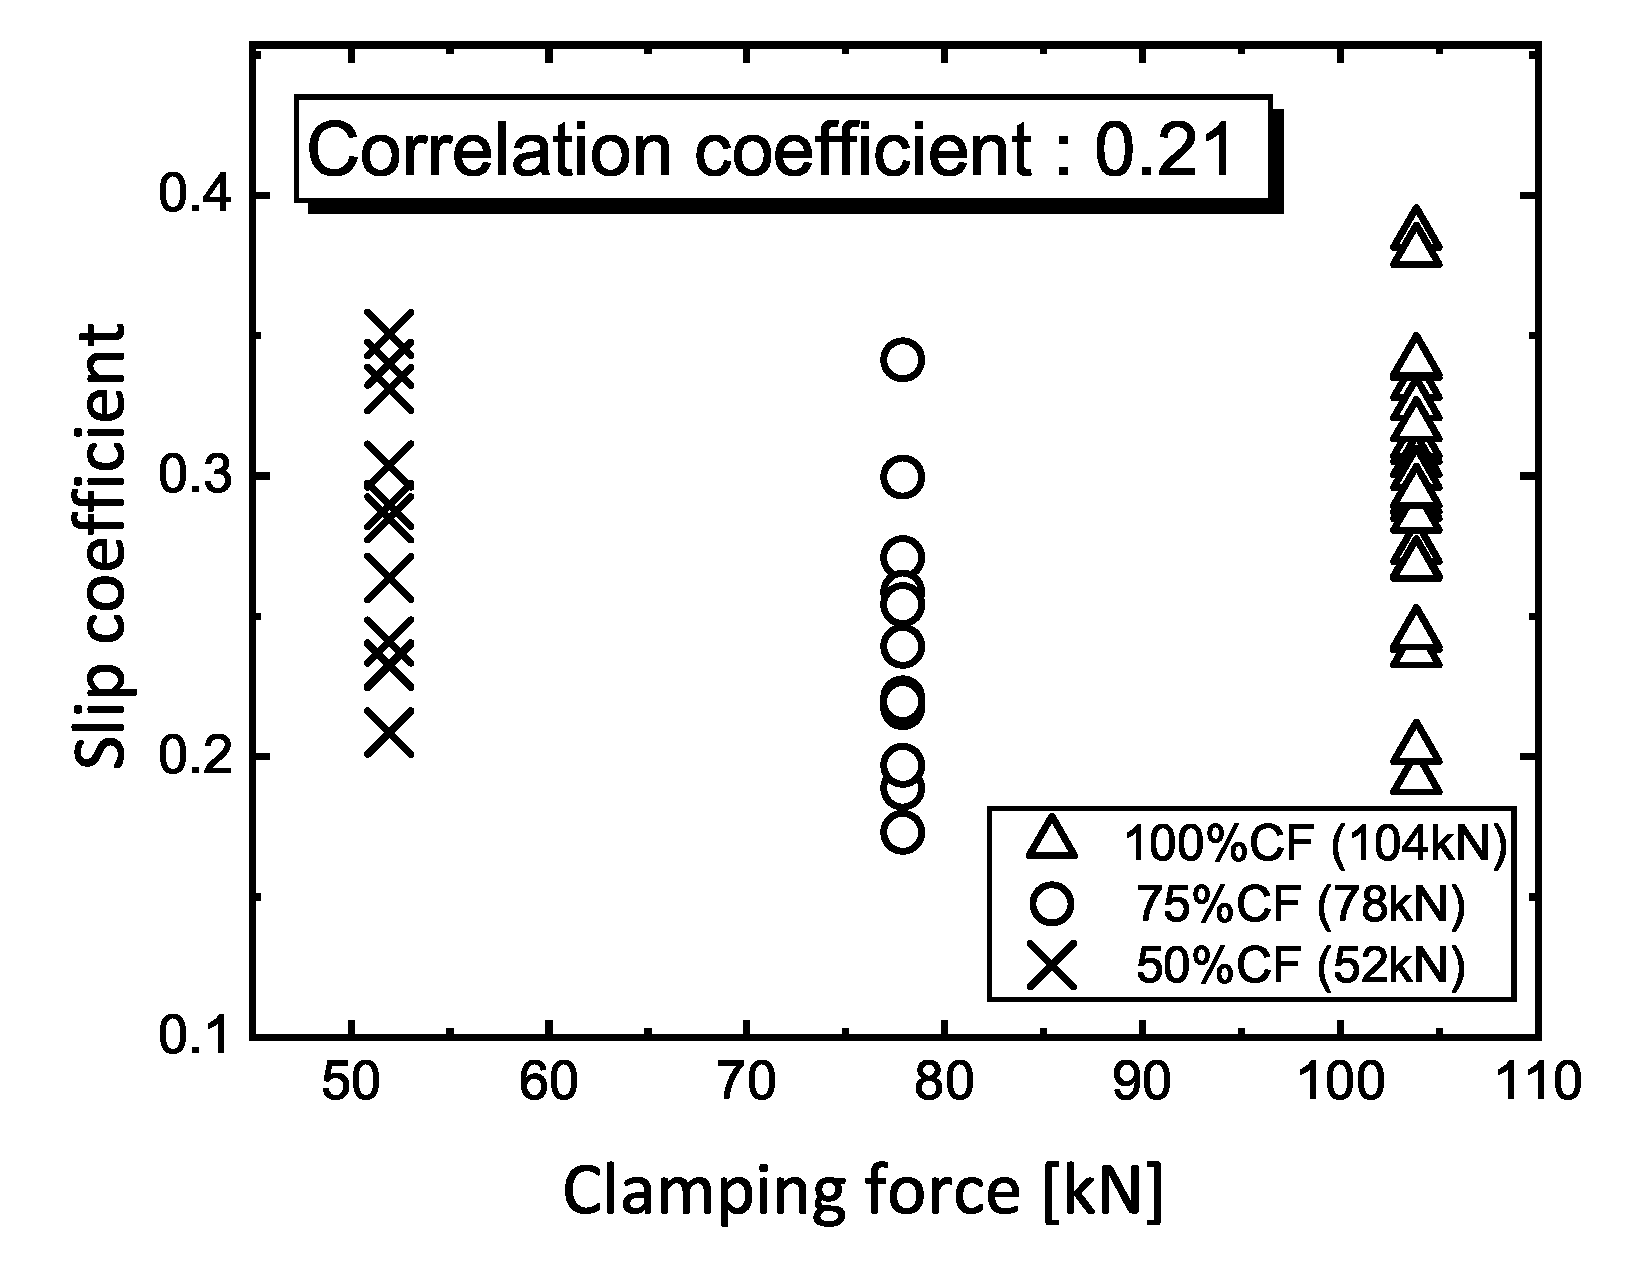
\includegraphics[width=\linewidth]{imgs/ch3/fig11.eps}
\caption{The relationship between the slip coefficient and the clamping force.}
\label{ch3fig11}
\end{minipage}
\begin{minipage}[t]{0.48\textwidth}
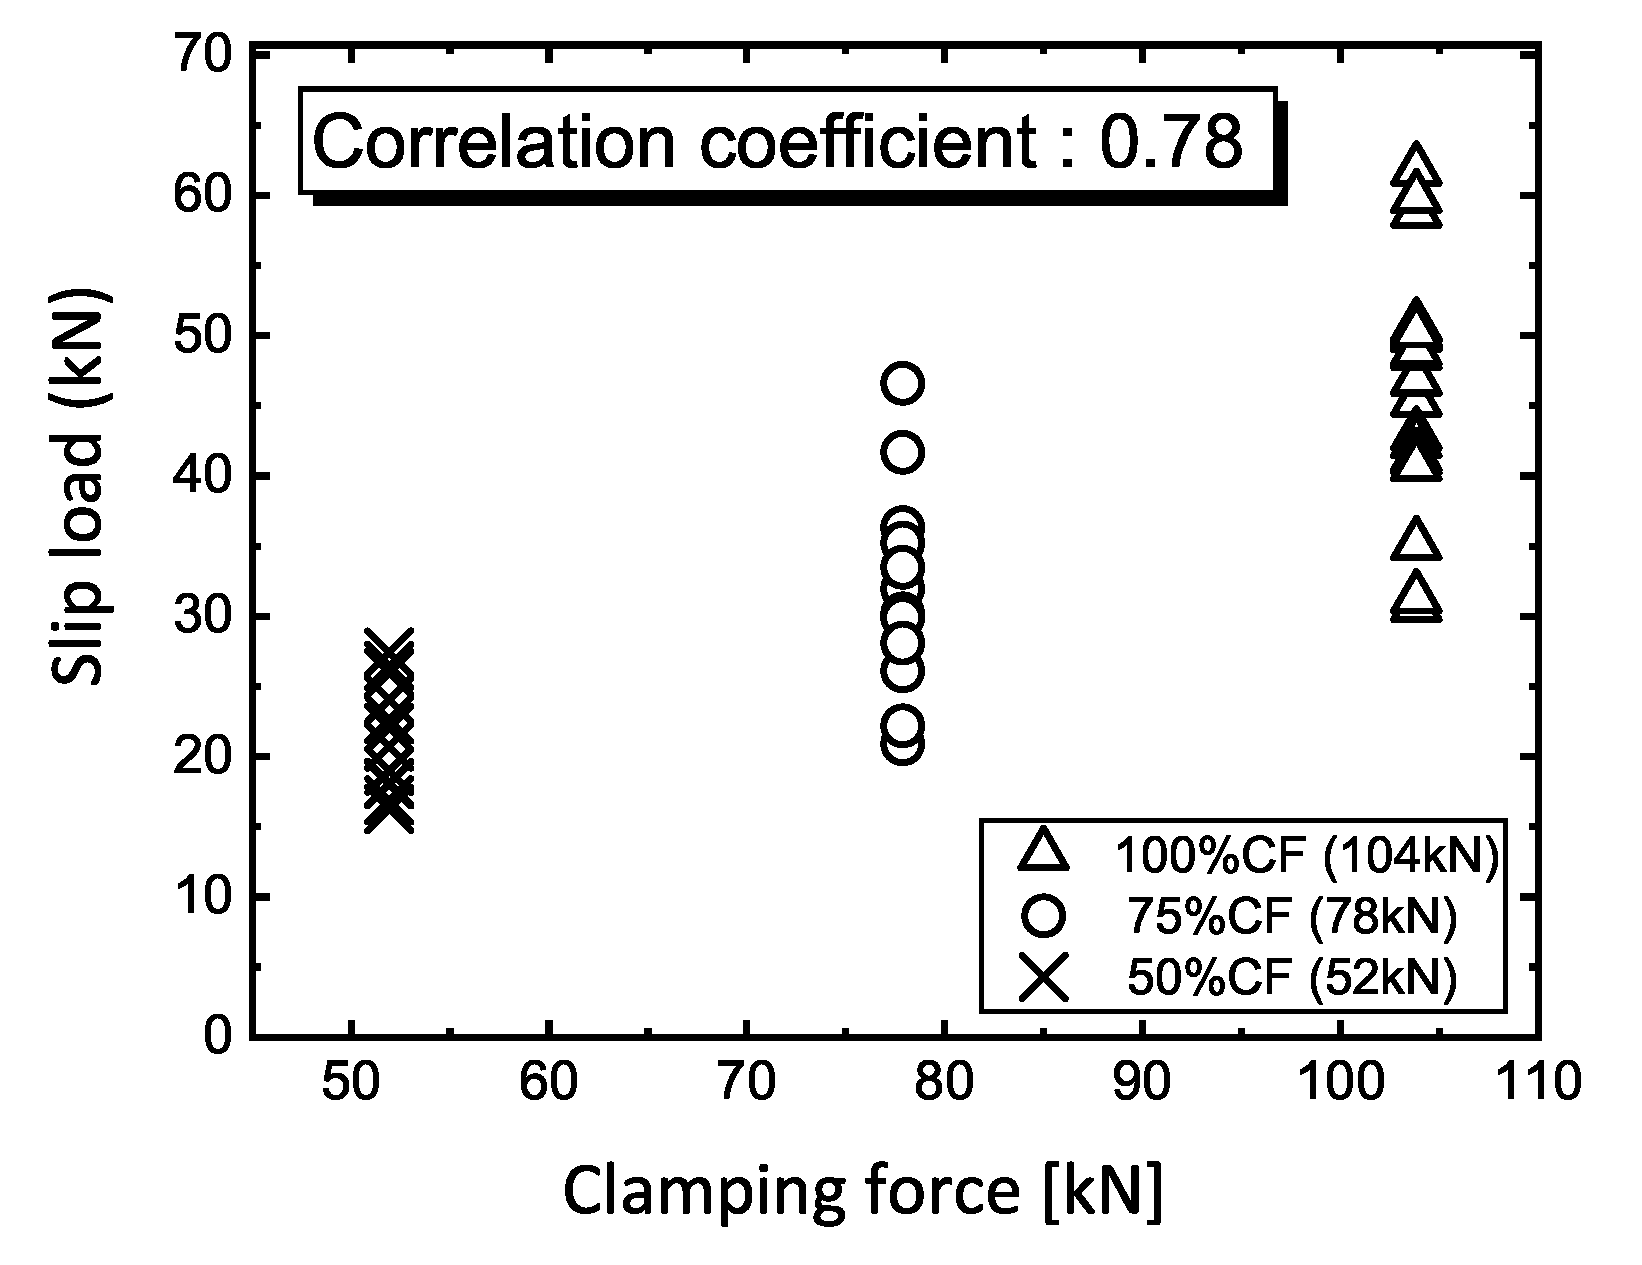
\includegraphics[width=\linewidth]{imgs/ch3/fig12.eps}
\caption{The relationship between the slip load and the clamping force.}
\label{ch3fig12}
\end{minipage}
\end{figure}

In addition, the average friction coefficient obtained is 0.295, which is 0.02 larger than the average slip coefficient of 0.274. The friction coefficient is calculated by dividing the load by the clamping force, which is taken when slippage has occurred. 

\subsection{Contact pressure distribution test}

The observation of the joint surface in section \ref{ch3sec2-1} revealed that the red lead surface distribution of specimens was much not uniform, and the red lead distribution of each specimen was also very different. In this study, a pressure distribution test is performed to investigate the influence of red lead distribution on the contact pressure and the slip coefficient. 

\subsubsection{Measuring methods}
A pressure measurement film is put into the joint surface, and then the standard clamping force is applied to the specimen by the screw-jack. When detected pressure, the film will be colored redder as the pressure increases.

\subsubsection{Measuring result}

Eight sets of specimens are conducted with a pressure distribution test. The pressure distribution was very uneven according to the aging condition of red lead paint, and the residual condition of red lead directly reflected the pressure distribution. Fig. \ref{ch3fig13} shows the pressure test results of the specimens' joint surface with a slip coefficient of 0.284 and the joint surface's condition before/after the slip test.


\begin{figure}
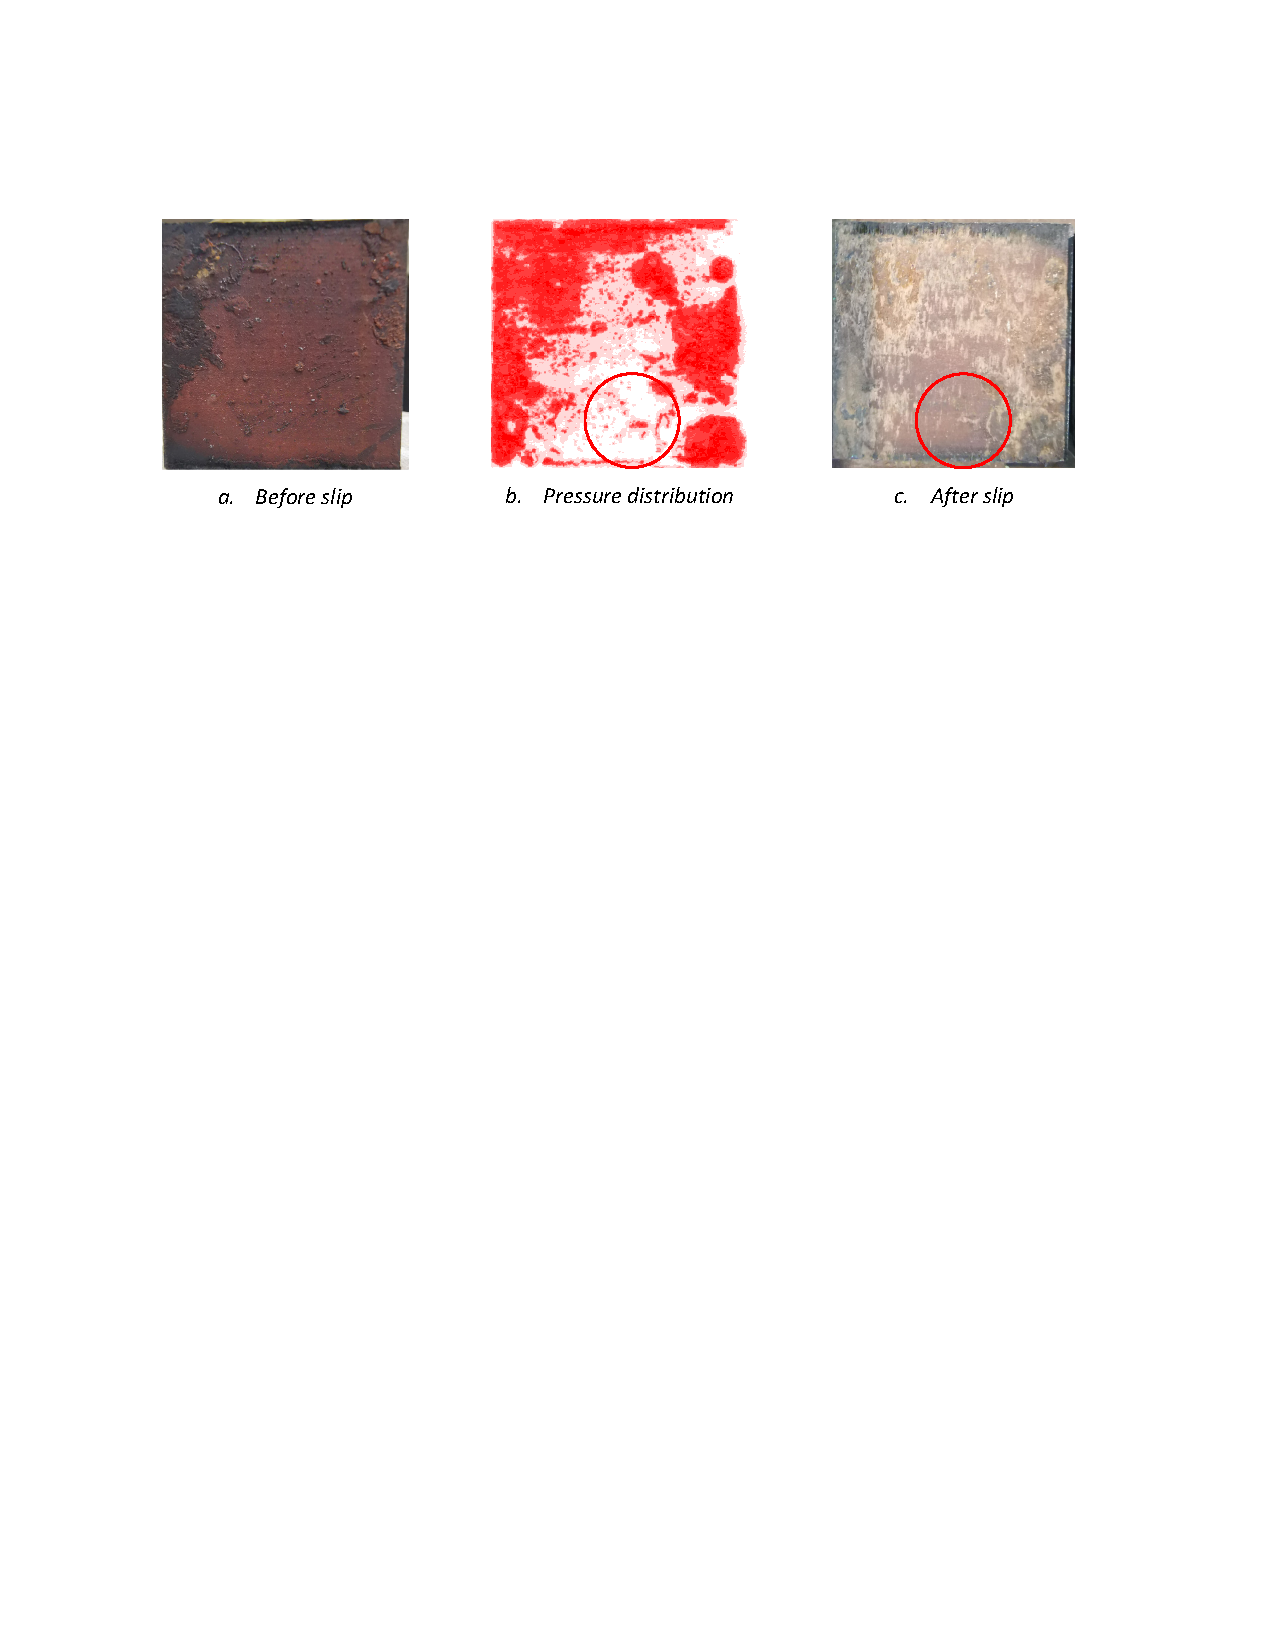
\includegraphics[width=\linewidth]{imgs/ch3/fig13.pdf}
\caption{Pressure contour figures and the condition before/after slip test.}
\label{ch3fig13}  
\end{figure}

As shown in Fig. \ref{ch3fig13}-b, the range marked with red is detected contact pressure area; the white areas have not detected contact pressure. The slip test assumes that the pressure is evenly distributed on the joint surface; however, the measuring results show that red lead paint's surface does not satisfy the average pressure distribution assumption.

As shown in Fig. \ref{ch3fig13}-c, after the slip test, the red lead paint on the joint surface was damaged. The traces of the slippage can be clearly seen. However, there are no traces of slippage near the marked red circle. The joint surface friction condition was very similar to the pressure distribution, as shown in Fig. \ref{ch3fig13}-b. It can be inferred that the white areas where no pressure is detected have no effective resistance to the friction and can be defined as the invalid contact area. On the contrary, the effective contact area is defined as where the contact pressure is detected. The effective contact pressure $σ_e$ is calculated by the effective contact area and clamping force.

\begin{equation}
    σ_e=N_0/S_e
\end{equation}
Where $N_0$ is clamping force;$ S_e$ is effective contact area. 

\begin{figure}
\centering
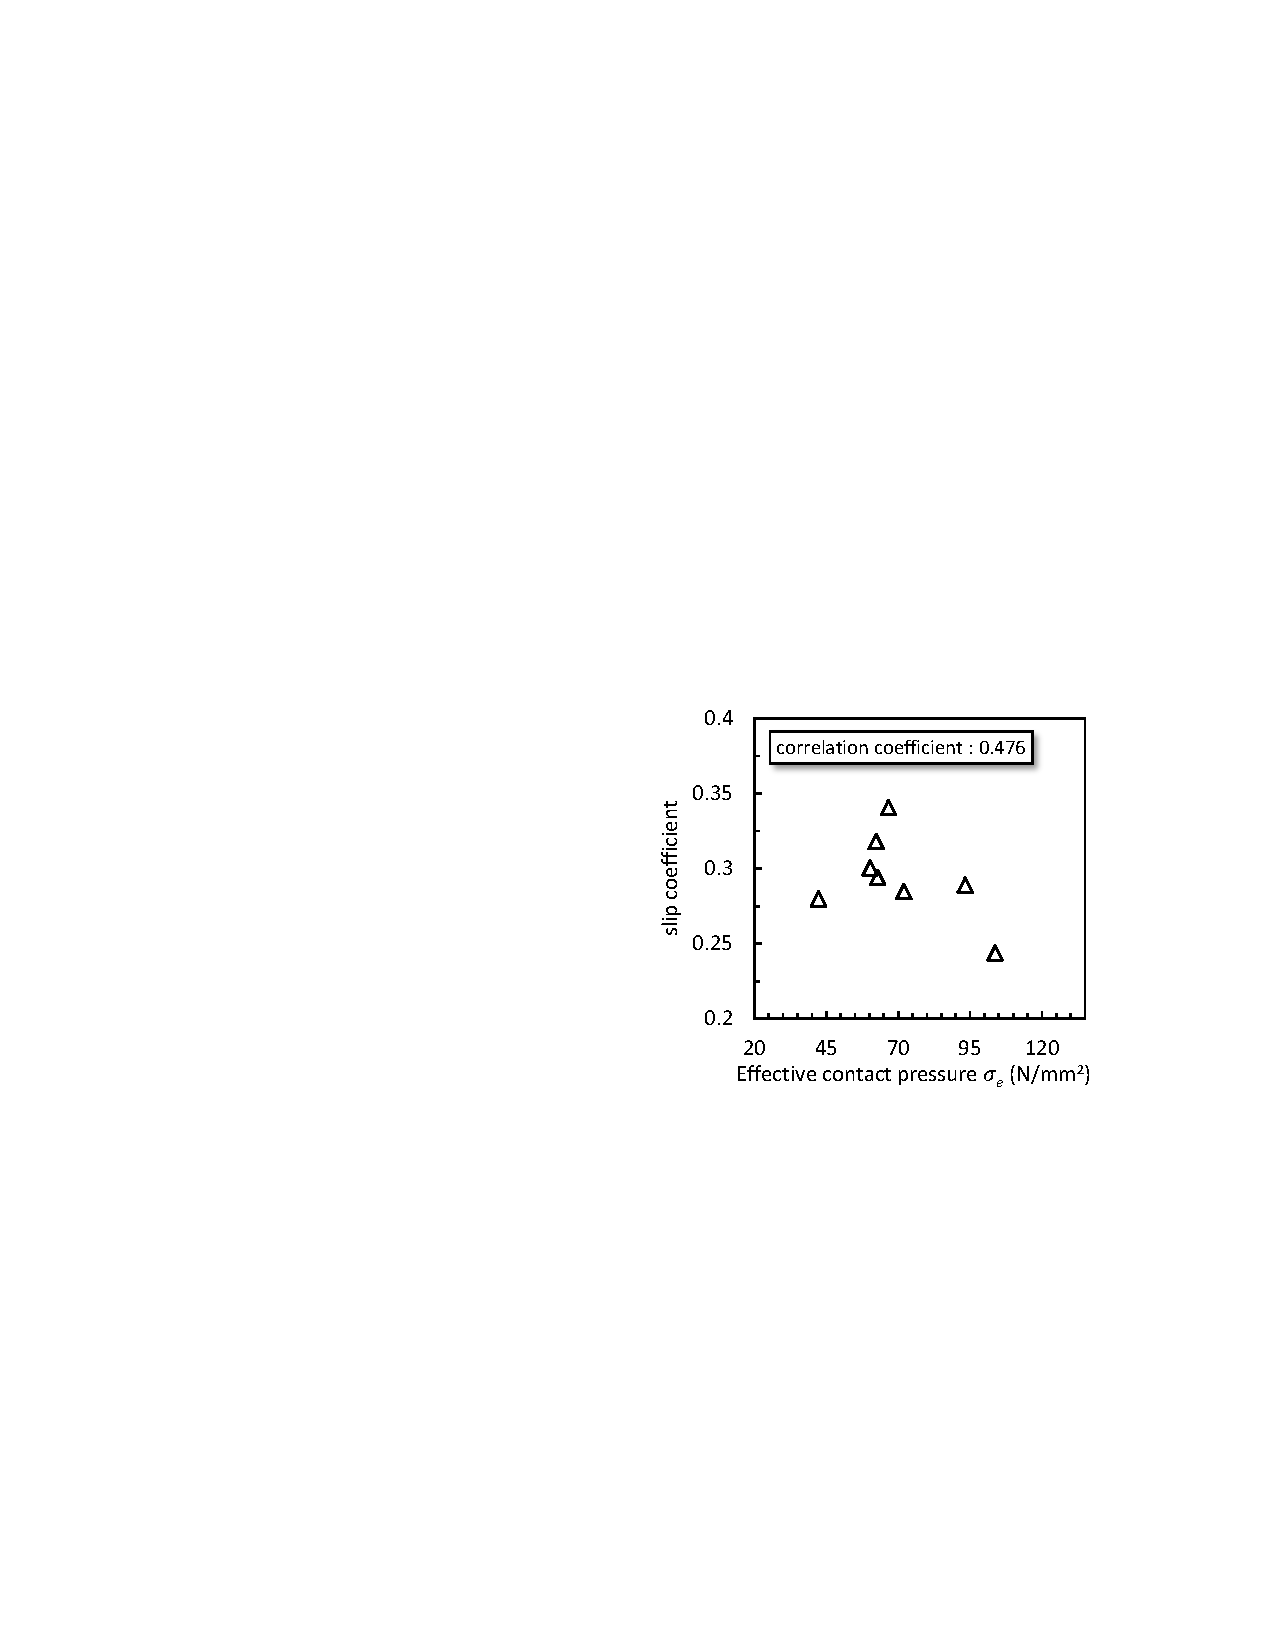
\includegraphics[width=0.65\linewidth]{imgs/ch3/fig14.pdf}
\caption{The relationship between slip coefficient and effective contact pressure}
\label{ch3fig14}  
\end{figure}

The relationship between slip coefficient and the effective contact pressure is shown in Fig. \ref{ch3fig14}. The effective contact area for each specimen is different, so although the same clamping force they have, calculated effective contact pressure is different. The correlation coefficient between the slip coefficient and the effective contact pressure is calculated as 0.476. No apparent relationship between the slip coefficient and the effective contact pressures has been observed. It could be considered that reason is the contact pressure was unevenly distributed in the effective contact area. Furthermore, the invalid pressure area and low contact pressure area do not effectively resist friction, and local slip has likely occurred. 


\subsection{Summarize for the slip coefficient}
In this study, the joint part cut out from a 90-year-old riveted bridge's cross-beam. It evaluated the riveted joint surface's aging condition with red lead by microscope observation and chemical analysis. The slip and pressure distribution tests are also conducted to investigate the joint surface's slip coefficient of the riveted joints and the pressure distribution of riveted joints' surface. 

Given the results of the present research, the obtained conclusions are as follows: 

\begin{itemize}
    \item The distribution of red lead on the joint surface is not flat, the adhesion of the red lead has deteriorated, and the black oxide on the surface of the steel can be observed. In addition to the red lead film, vinyl acetate was also discovered by the FT-IR spectra analysis. 

    \item The average slip coefficient was 0.274, and the coefficient of variation was 0.191.-2σ is 0.169. The 95\% confidence interval for the slip coefficient is 0.259-0.289. 

    \item According to the relationship between the slip coefficient and clamping force, it has been confirmed that the change of the clamping force will not affect the slip coefficient.

    \item The pressure distribution test could be concluded that due to the joint surface is not flat, the pressure distribution is also very uneven, and very high pressure is generated locally. On the contrary, there is no effective pressure applied in some places called an invalid contact area. Besides, the slip coefficient has no obvious relationship with effective contact pressures.
    
\end{itemize}
\chapter{Experiment of Rivet-HSB hybrid Connection}
\label{ch4}

%%%%%%%%%%%%%%%%%%%%%%%%%%%%%%%%%%%%%%%
% IMPORTANT
\begin{spacing}{1.25} %THESE FOUR
\minitoc % LINES MUST APPEAR IN
\end{spacing} % EVERY
\onehalfspacing % CHAPTER
% COPY THEM IN ANY NEW CHAPTER
%%%%%%%%%%%%%%%%%%%%%%%%%%%%%%%%%%%%%%%

\kant[1-2]
\chapter{Numerical Analysis of IFB-HSB hybrid Connection}
\label{ch5}

%%%%%%%%%%%%%%%%%%%%%%%%%%%%%%%%%%%%%%%
% IMPORTANT
\begin{spacing}{1.25} %THESE FOUR
\minitoc % LINES MUST APPEAR IN
\end{spacing} % EVERY
\onehalfspacing % CHAPTER
% COPY THEM IN ANY NEW CHAPTER
%%%%%%%%%%%%%%%%%%%%%%%%%%%%%%%%%%%%%%%

\kant[1-2]
\chapter{Experiment of IFB-HSB hybrid Connection}
\label{ch6}

%%%%%%%%%%%%%%%%%%%%%%%%%%%%%%%%%%%%%%%
% IMPORTANT
\begin{spacing}{1.25} %THESE FOUR
\minitoc % LINES MUST APPEAR IN
\end{spacing} % EVERY
\onehalfspacing % CHAPTER
% COPY THEM IN ANY NEW CHAPTER
%%%%%%%%%%%%%%%%%%%%%%%%%%%%%%%%%%%%%%%

\section{Introduction}

Chapter \ref{ch5} presented a method that combined the bearing-type bolts at both ends of the friction type bolted joint (hereinafter known as the Hybrid bolted joint). The result showed that the 12-row hybrid joint could improve about 20\% slip load than the 12-row friction bolted joint. However, this result is based on numerical analysis and does not take into account the actual assembly of interference fit bolts.

This study focuses on Interference fit bolts assembled at both ends of friction type bolted joint. Tensile tests were performed with three specimens: friction type bolted joints (hereafter known as friction joint), hybrid joints and hybrid joints with Interference fit bolts without preload application. The purpose of this study is to elucidate the load transmission mechanism of the hybrid joints, the slip resistance, and to verify whether the Interference fit bolts can be assembled in the friction joints to improve the strength of the joints.


\section{Interference fit bolt}

A specialized high-strength bolt for bearing-type connection (hereafter known as the Interference fit bolt) is present \cite{Fisher2001,bolt-bearing,Chen2023MechanicalConnections} as shown in Fig. \ref{ch6fig-onebbolt}. Interference fit bolts of B10T grade was utilized (courtesy of Kobelco Bolt, Ltd.) and meets the strength requirements of an F10T bolt according to the JIS-B1186 standard \cite{JISbolt}, which is equivalent to ASTM-A490 \cite{ASTM-bolt} \& Grade 10.9 \cite{ISO-bolt} and possesses the unique feature of an axially ribbed shank. When the bolt is hammered into a hole, the rib undergoes plastic deformation to ensure a tight fit and prevents excessive slipping. Interference fit bolts are employed for retrofitting steel bridge piers that have fatigue damage or corrosion by attaching the patch plate \cite{Anami-bbolt-ate}. This is because initial imperfections or corrosion leads to uneven steel plate surfaces, making it impossible for the patch plate of the friction type bolted connection to effectively contact the steel surface and transmit force. And Interference fit bolts also can reduce the fatigue damage in bolt holes, and increasing their fatigue strength \cite{Guo20205}. However, Interference fit bolts are rarely used on other bridge parts owing to their stringent installation requirements. 

\begin{figure}[htbp]
    \centering
    \includegraphics[width=0.5\textwidth]{imgs/ch6/oneBbolt.png}
    \caption{Interference fit bolt for Bearing-type connection (M22, Diameter = 23.5mm, Courtesy of Kobelco Bolt, Ltd.)}
    \label{ch6fig-onebbolt}
\end{figure}

For bearing-type bolted connections, AASHTO LRFD BDS 2020 \cite{AASHTO2020} defines it as a strength limit state only for joints subjected to axial compression or joints on bracing members. Both Eurocode3 EN 1993-1-8:2021 \cite{eurocode3-21}and GB50017-2017 \cite{gb50017-2017}define that it should be designed in the same way as friction-type bolted connections, and define the serviceability limit state as slip resistance and the bearing resistance as the ultimate limit state. However, Eurocode 3 allows the bearing resistance of resin and slip resistance of injection bolts to be accumulated for design under the serviceability limit state, and Japanese's JSHB-2017 \cite{douji2017} states that bearing type bolted connections could be designed to meet serviceability limit state by bearing resistance. 


\section{Experiment}

\subsection{Material test}

The material test specimens were prepared in accordance with JIS Z 2241 2011\cite{JIStest}. Material tests were conducted on three steel specimens of 50 mm and 28 mm thickness, respectively. The summary results are shown in Table \ref{tab-mtresult}. Plan view after material test as shown in Fig. \ref{fig-mt-1}. \par

and the load-strain relationships for the 50 mm thickness specimens are shown in Fig. \ref{fig-mt50-ls}

\begin{figure}[htbp]
    \centering
    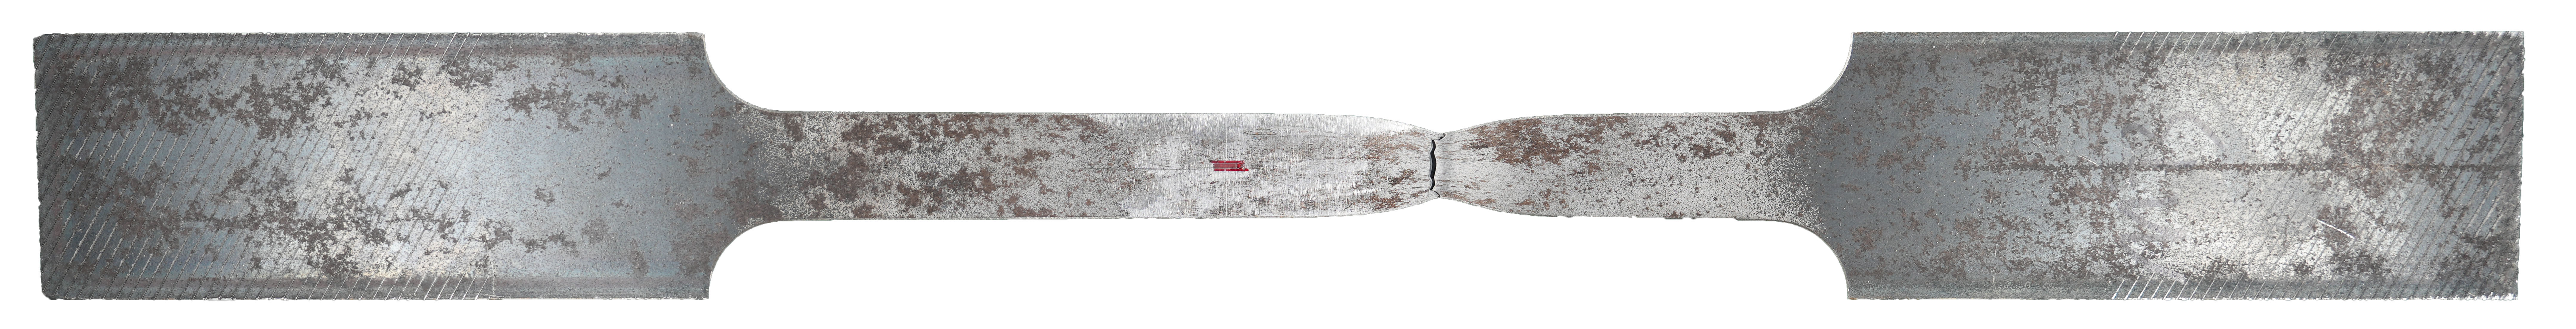
\includegraphics[width=0.8\textwidth]{imgs/ch6/mt-1.jpg}
    \caption{Plan view after material test}
    \label{fig-mt-1}
\end{figure}

\begin{figure}[htbp]
    \centering
    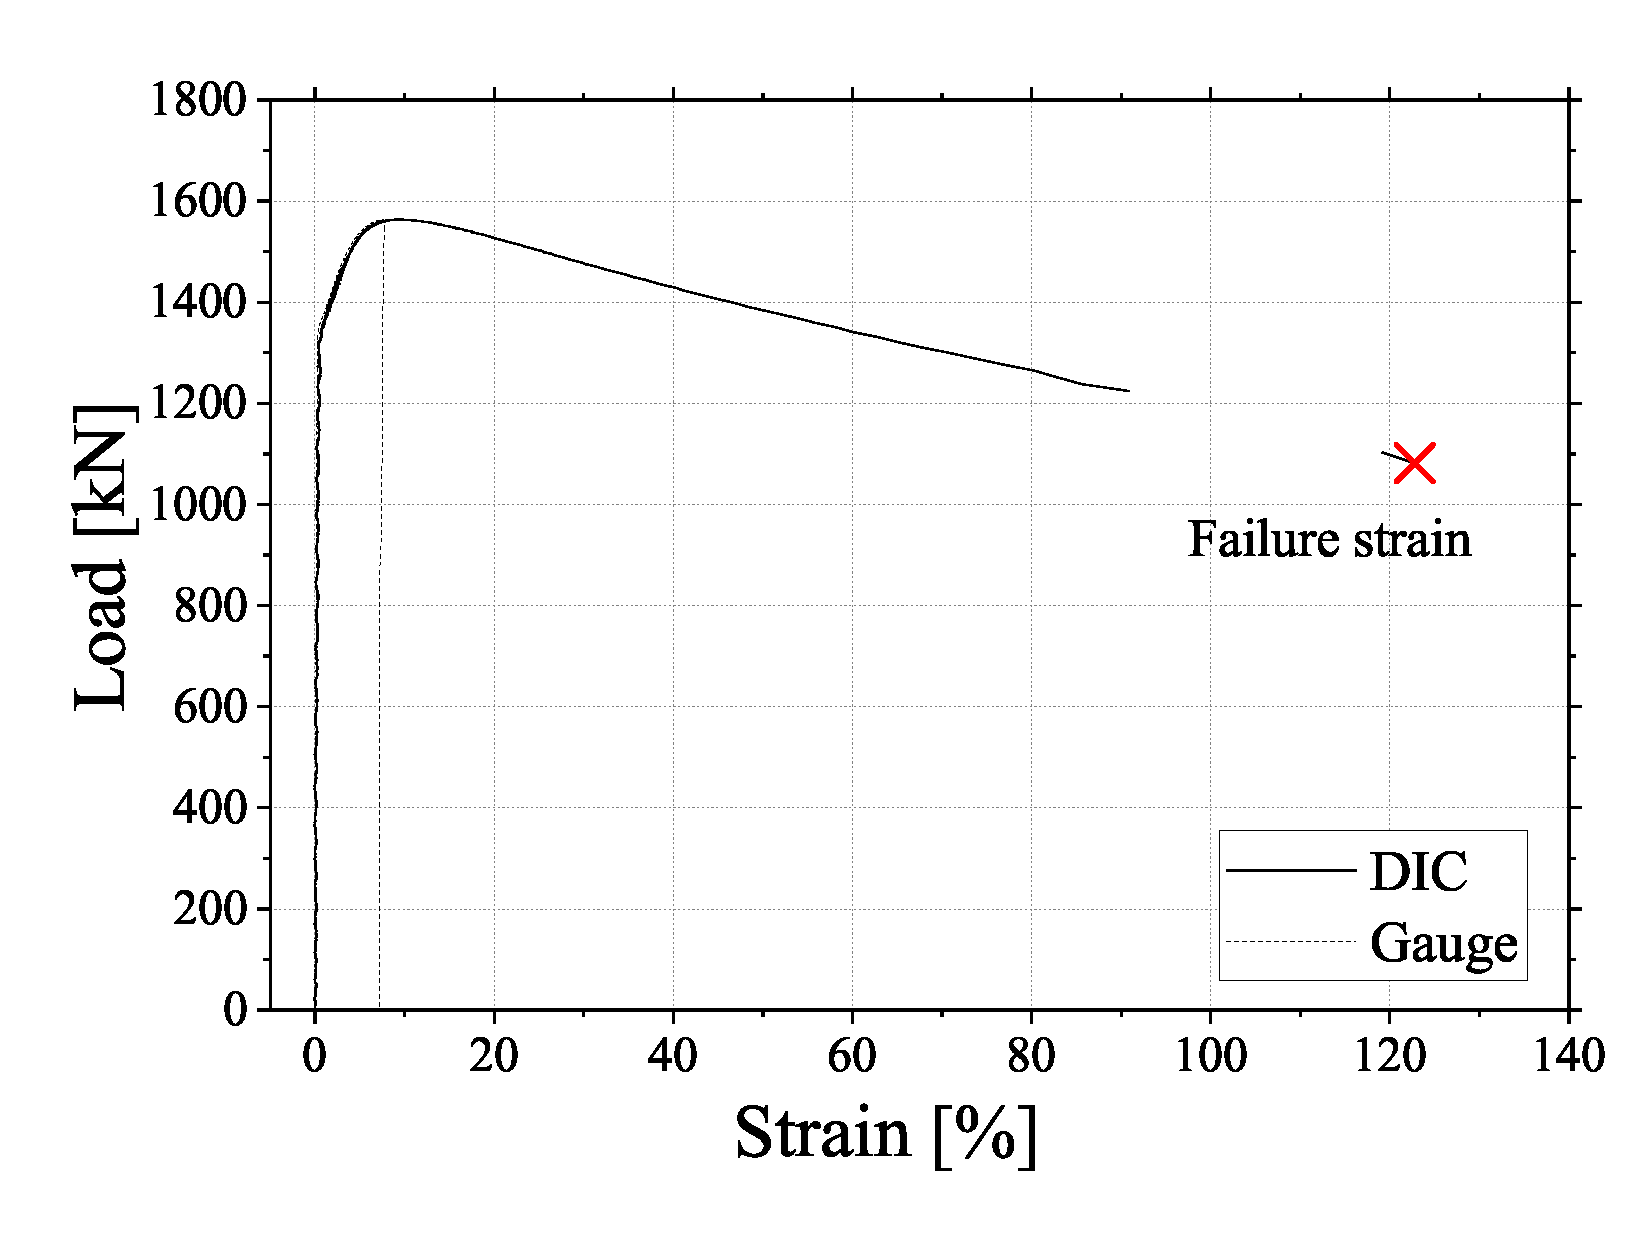
\includegraphics[width=0.6\textwidth]{imgs/ch6/mt50-LS.eps}
    \caption{The relationship between Load and Strain}
    \label{fig-mt50-ls}
\end{figure}

\begin{table}[htbp]
\centering
\caption{Material test results}
\label{tab-mtresult}
\begin{tabular}{@{}ccccccc@{}}
\toprule
\multirow{2}{*}{\begin{tabular}[c]{@{}c@{}}Component\\ name\end{tabular}} & \multicolumn{2}{c}{\begin{tabular}[c]{@{}c@{}}Plate\\ 28 mm \end{tabular}} & \multicolumn{2}{c}{\begin{tabular}[c]{@{}c@{}}Plate\\50 mm\end{tabular}} & \begin{tabular}[c]{@{}c@{}}Interference fit \\ bolt (B10T)\end{tabular} & \begin{tabular}[c]{@{}c@{}}High-strength \\ bolt (F10T)\end{tabular} \\ \cmidrule(l){2-7} 

& \begin{tabular}[c]{@{}c@{}}Inspection \\ Certificate\end{tabular} & \begin{tabular}[c]{@{}c@{}}Tensile \\ test\end{tabular} & \begin{tabular}[c]{@{}c@{}}Inspection \\ Certificate\end{tabular} & \begin{tabular}[c]{@{}c@{}}Tensile \\ test\end{tabular} & \multicolumn{2}{c}{\begin{tabular}[c]{@{}c@{}}Inspection \\ Certificate\end{tabular}} \\ \midrule

\begin{tabular}[c]{@{}c@{}}Yield Strength\\ {[}$N/mm^2${]}\end{tabular} & 536 & 525.5 & 549 & 548.6 & 1025 & 998 \\
\begin{tabular}[c]{@{}c@{}}Ultimate Strength\\ {[}$N/mm^2${]}\end{tabular} & 633 & 619.5 & 646 & 635.5 & 1073 & 1075 \\
\begin{tabular}[c]{@{}c@{}}Young's modulus $E$\\ {[}$KN/mm^2${]}\end{tabular} & - & 209 & - & 213 & - & - \\
Poisson's ratio $v$ & - & 0.274 & - & 0.269 & - &- \\
\begin{tabular}[c]{@{}c@{}}Elongation\\ {[}$\%${]}\end{tabular} & 26 & - & 46 & - & 19& 19\\ \bottomrule
\end{tabular}
\end{table}

\subsection{Standard slip test for measurement the slip coefficient}

The geometry of the standard slip test specimen is shown in Fig. \ref{fig-sliptest}, and the structural characteristics are shown in Table \ref{tab-sizeslip}. The geometry was prepared with reference to the high-strength bolt design, construction, and maintenance guidelines \cite{shishin2009}.

\begin{figure}[htbp]
    \centering
    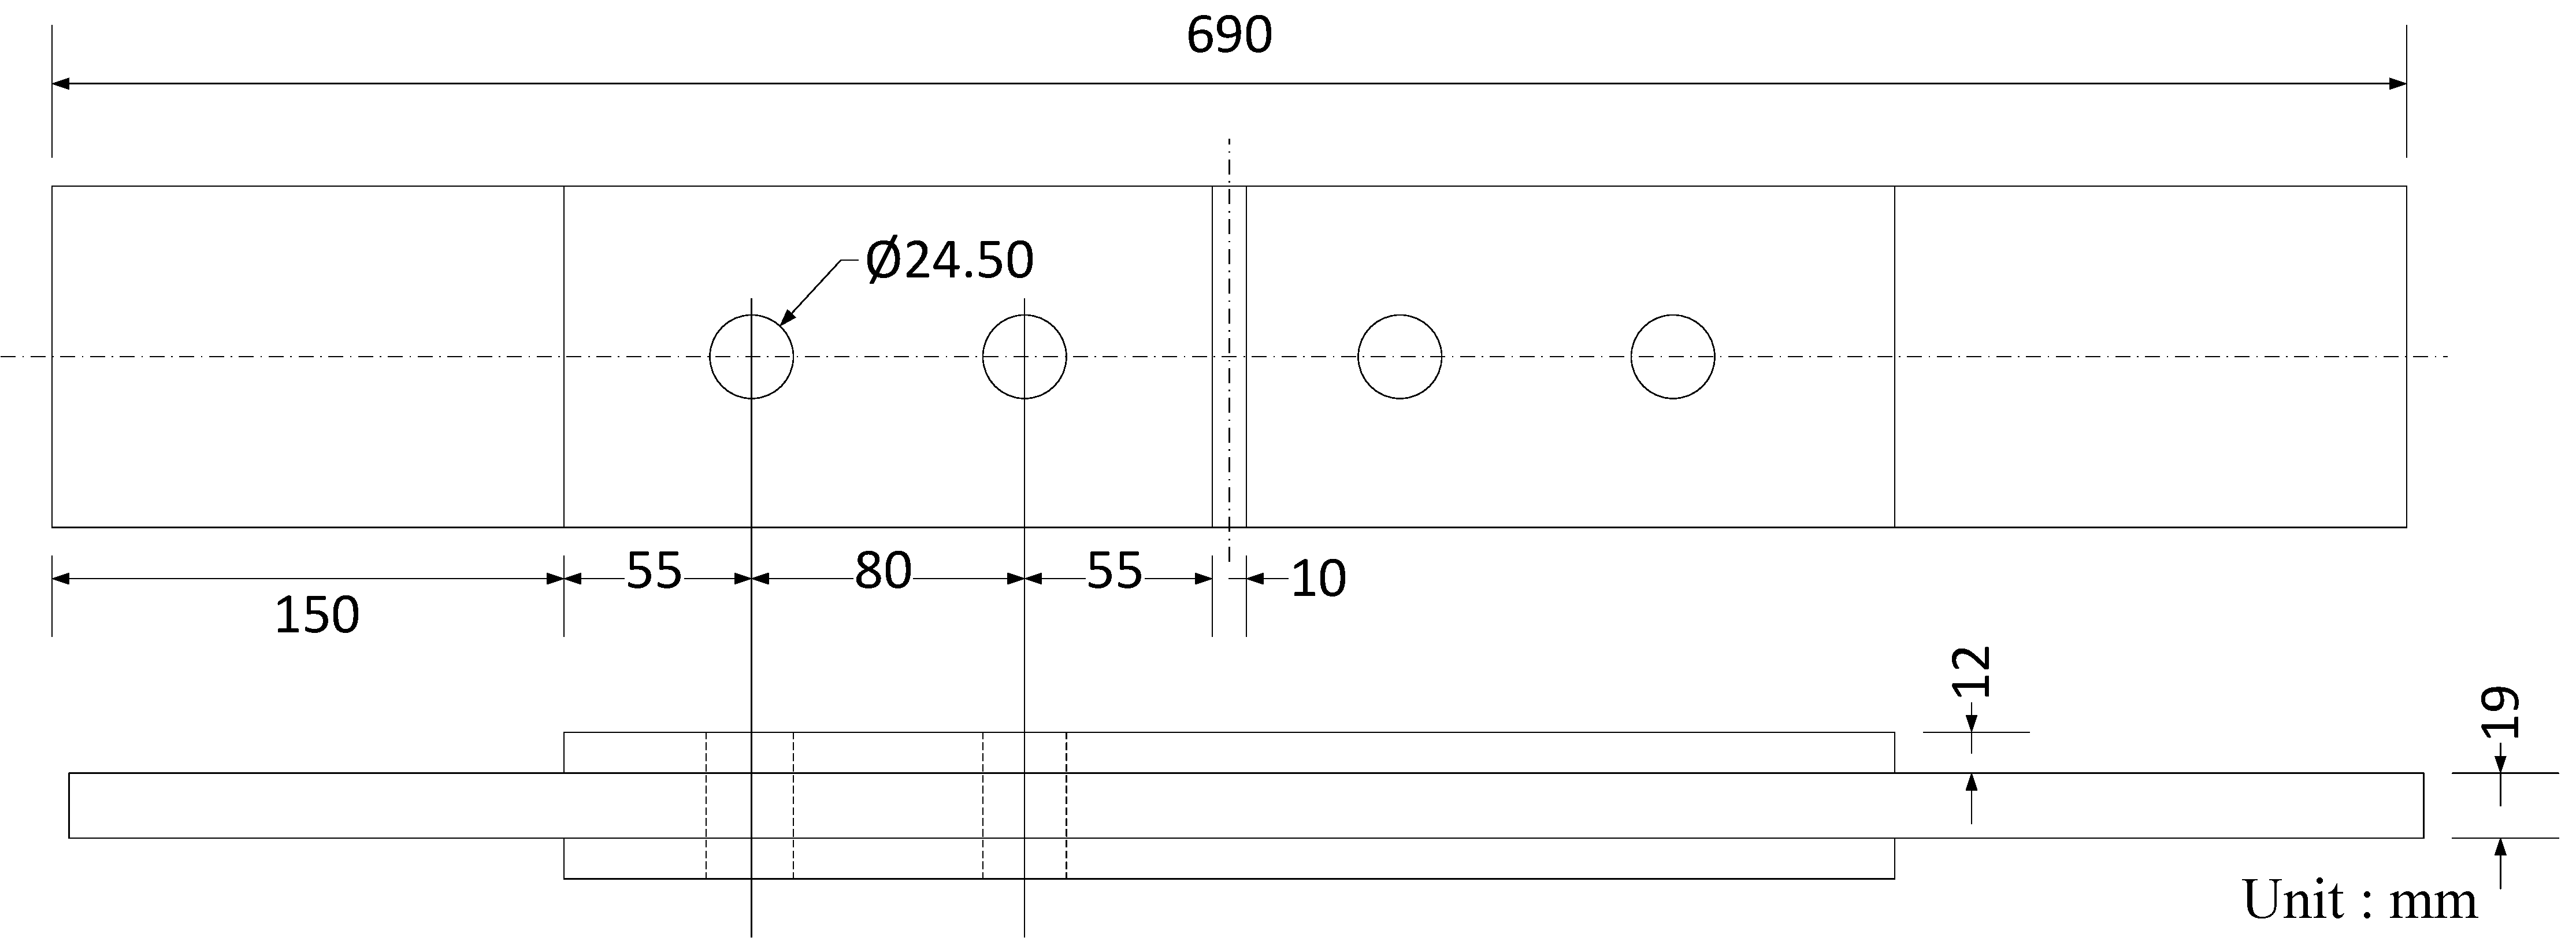
\includegraphics[width=0.85\linewidth]{imgs/ch6/slip-test.pdf}
    \caption{Shape of standard slip specimen}
    \label{fig-sliptest}
\end{figure}

\begin{table}[htbp]
\centering
\caption{Shape of standard slip specimen}
\label{tab-sizeslip}
\begin{tabular}{@{}cccccccccc@{}}
\toprule
 \begin{tabular}[c]{@{}c@{}}Bolt \\ grade\end{tabular}&
  \begin{tabular}[c]{@{}c@{}}$d$\end{tabular} &
  \begin{tabular}[c]{@{}c@{}}$d_0$\end{tabular} &
  \begin{tabular}[c]{@{}c@{}}Steel grade\end{tabular} &
  \begin{tabular}[c]{@{}c@{}}$f_y$\end{tabular} &
  \begin{tabular}[c]{@{}c@{}} $t_m$\end{tabular} &
  \begin{tabular}[c]{@{}c@{}}$t_s$\end{tabular} &
  \begin{tabular}[c]{@{}c@{}} $w$\end{tabular} &
  \begin{tabular}[c]{@{}c@{}}$e_1$\end{tabular} &
  \begin{tabular}[c]{@{}c@{}}$p_1$\end{tabular} 
  \\ \midrule
F10T & 22 & 24.5 & SM490Y & 355 & 19 & 12 & 100 & 55 & 80
\\ \bottomrule
\end{tabular}
\end{table}

where, $t_m$ is the thickness of main plate, $t_s$ is the thickness of splice plate, $w$ is the width of mian plate, $e_1$ is the end distance from bolt hole, $p_1$ is the bolt spacing. 

The test method for the standard slip test is shown below.

\begin{enumerate}
    \item The number of specimens shall be three. One side of the specimen is the test side and the other side is the fixed side. The bolts on the fixing side should be retightened by $10\%$ to prevent slippage at the test end. \\
    The slip coefficient $\mu$ is calculated by the following equation.
    \begin{equation}
    \mu = \frac{P}{m\times n \times N}
    \end{equation}
    where $P$: slip load measured by slip test, $m$: number of joint faces (=2), $m$: number of bolts (=2), $N$: design bolt axial force
    
    \item The joint surface treatment shall be the same as that of the adopted joint.
    In the 
    \item test, tensile loading is performed while measuring the relative displacement between the main plate and splice plate, and if no clear slip occurs, the measured relative displacement is used to determine the slip load (here, the relative displacement is used to determine the slip load). (In this case, slip is determined when the relative displacement reaches 0.2 mm.)
    \item The axial force introduced into the bolt is based on the standard axial force, and the test is conducted at least 12 hours after the bolt has been tightened, taking into account the effect of relaxation.
\end{enumerate}

The result of slip coefficient test as shown in table \ref{tab-slipcoef}, both the bolt preload and the slip coefficient have a low variation.

\begin{table}[htbp]
\centering
\caption{Result of slip coefficient test}\label{tab-slipcoef}
\begin{tabular}{@{}ccccc@{}}
\toprule
\multirow{2}{*}{Name} & \multicolumn{2}{c}{Preload} & \multirow{2}{*}{Slip load} & \multirow{2}{*}{Slip Coefficient} \\ \cmidrule(lr){2-3}
 & Before loading & Avg. &  &  \\ \midrule
\multirow{2}{*}{test-1} & 108.58 & \multirow{2}{*}{105.6} & \multirow{2}{*}{332.2} & \multirow{2}{*}{0.786} \\
 & 102.74 &  &  &  \\
\multirow{2}{*}{test-2} & 107.18 & \multirow{2}{*}{107.6} & \multirow{2}{*}{352.4} & \multirow{2}{*}{0.819} \\
 & 108.42 &  &  &  \\
\multirow{2}{*}{test-3} & 107.18 & \multirow{2}{*}{107.8} & \multirow{2}{*}{348.4} & \multirow{2}{*}{0.808} \\
 & 108.42 &  &  &  \\
Mean &  &  &  & 0.804 \\
Standard Deviation &  &  &  & 0.017 \\ \bottomrule
\end{tabular}
\end{table}


\subsection{Experiment detail}

The experimental specimen dimensions shown in Fig. \ref{fig-dimens} were selected based on previous research\cite{KAMEI2000} on the investigation results of an actual bridge. The commonly occurring single-row 10-column arrangement was used as a reference. To investigate the mechanical behavior of slip and bearing of the joints, $\beta$ is set to 0.65 to prevent the joints from being affected by the cross-sectional yield of the main plate before slip.

The specimens were subjected to loading using a hydraulic universal testing machine with a capacity of 2000kN (provided by Tokyo Testing Machine Co. Ltd.). Considering the testing machine's loading capacity, the specimen was scaled down to a size of 16/22. Static uniaxial tension testing was conducted. The loading rate was set to 1 kN/s until either the test machine capacity was reached or failure occurred in the net cross section of plate or shear of the bolt. The loading device is depicted in Fig. \ref{fig-setup}.

Fig. \ref{fig-mealoc} shows the locations where the relative displacement, joint deformatioin, and strain are measured. Clip displacement gauges are used to measure relative displacement. Joint deformation is measured using an LVDT. Strain is measured using a strain gauge and a camera. Additionally, random patterns are applied to the side-2 of joint to capture the strain and displacement on the lateral side of the joint using \ac{DIC} method. Validation of \ac{DIC} methods as shown in Fig. \ref{fig-dicresult}.

\begin{figure}[htbp]
    \centering
    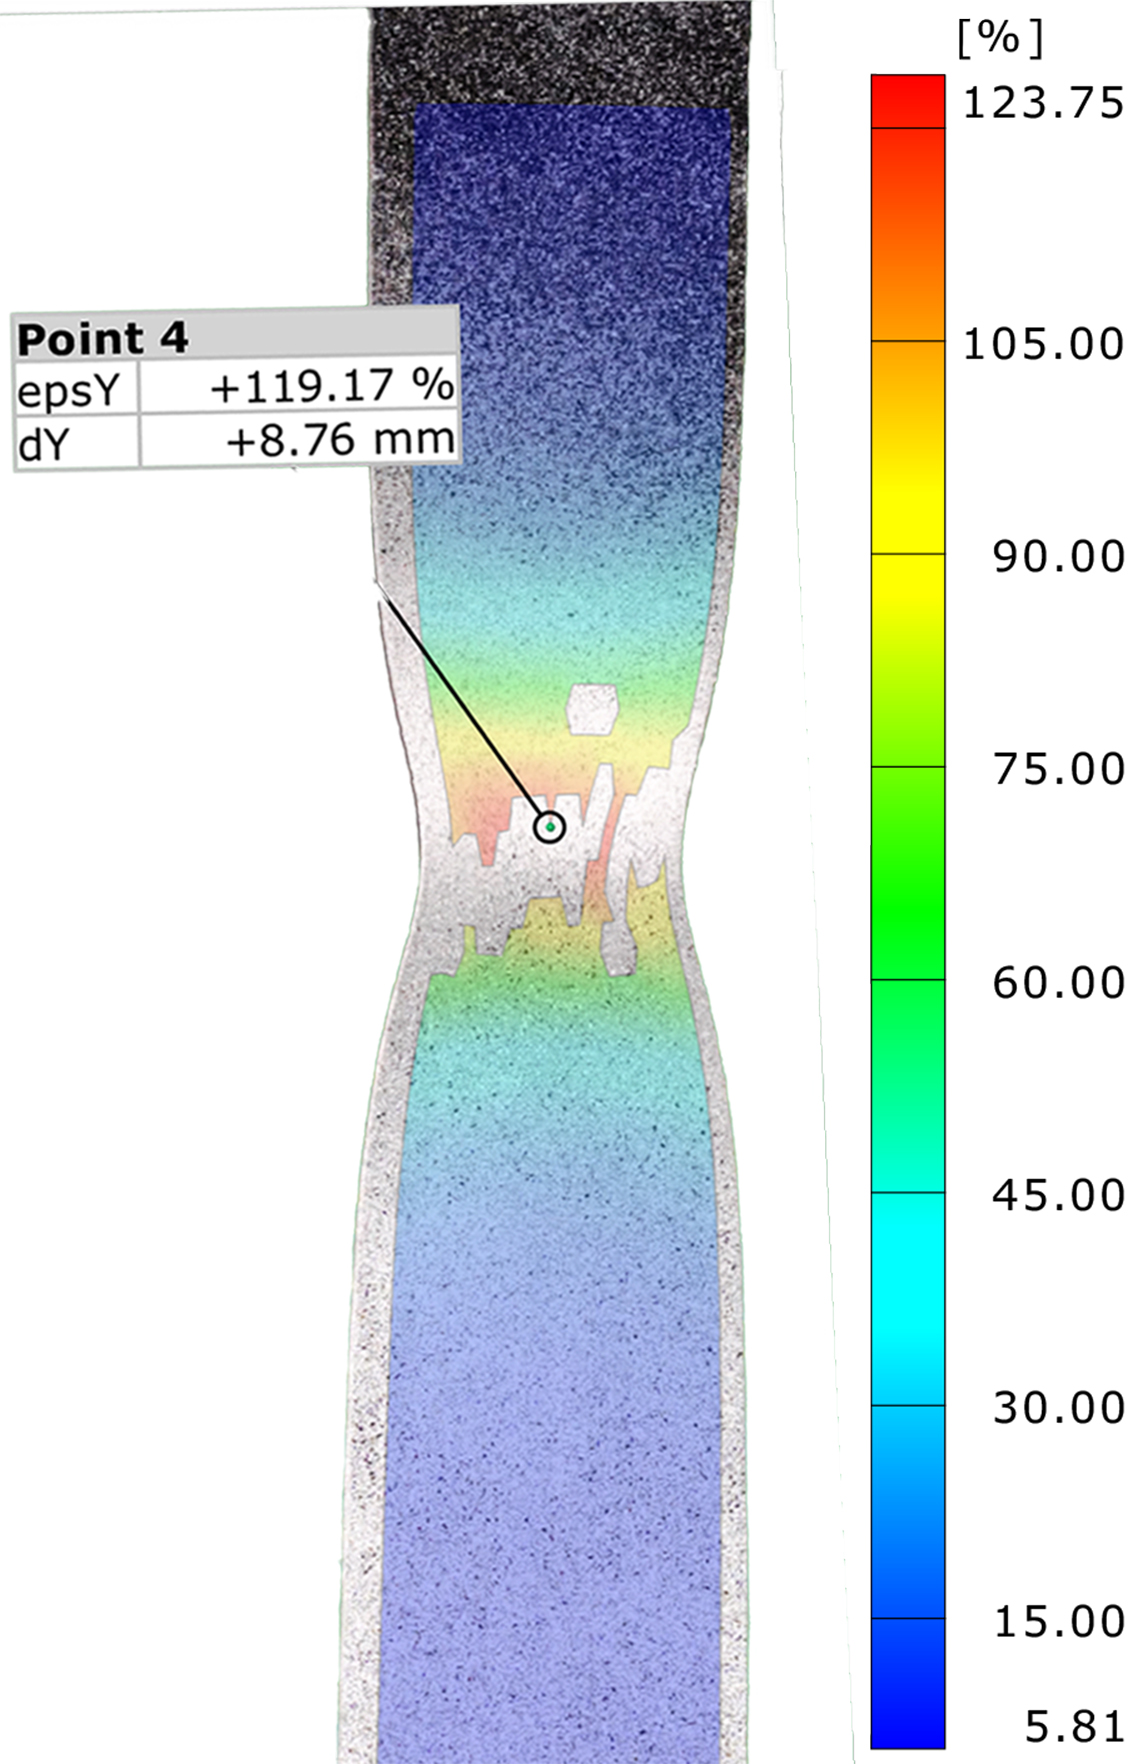
\includegraphics[width=0.4\textwidth]{imgs/ch6/DIC-RESULT.jpg}
    \caption{DIC-result}
    \label{fig-dicresult}
\end{figure}


According to JSHB\cite{douji2017}, the joint surface is coated with inorganic zinc-rich paint, with a presumed slip coefficient of 0.8, as determined from the slip factor test which arranged two bolts and have the same plate thickness and same faying surface condition as this test.

\begin{figure*}
    \centering
    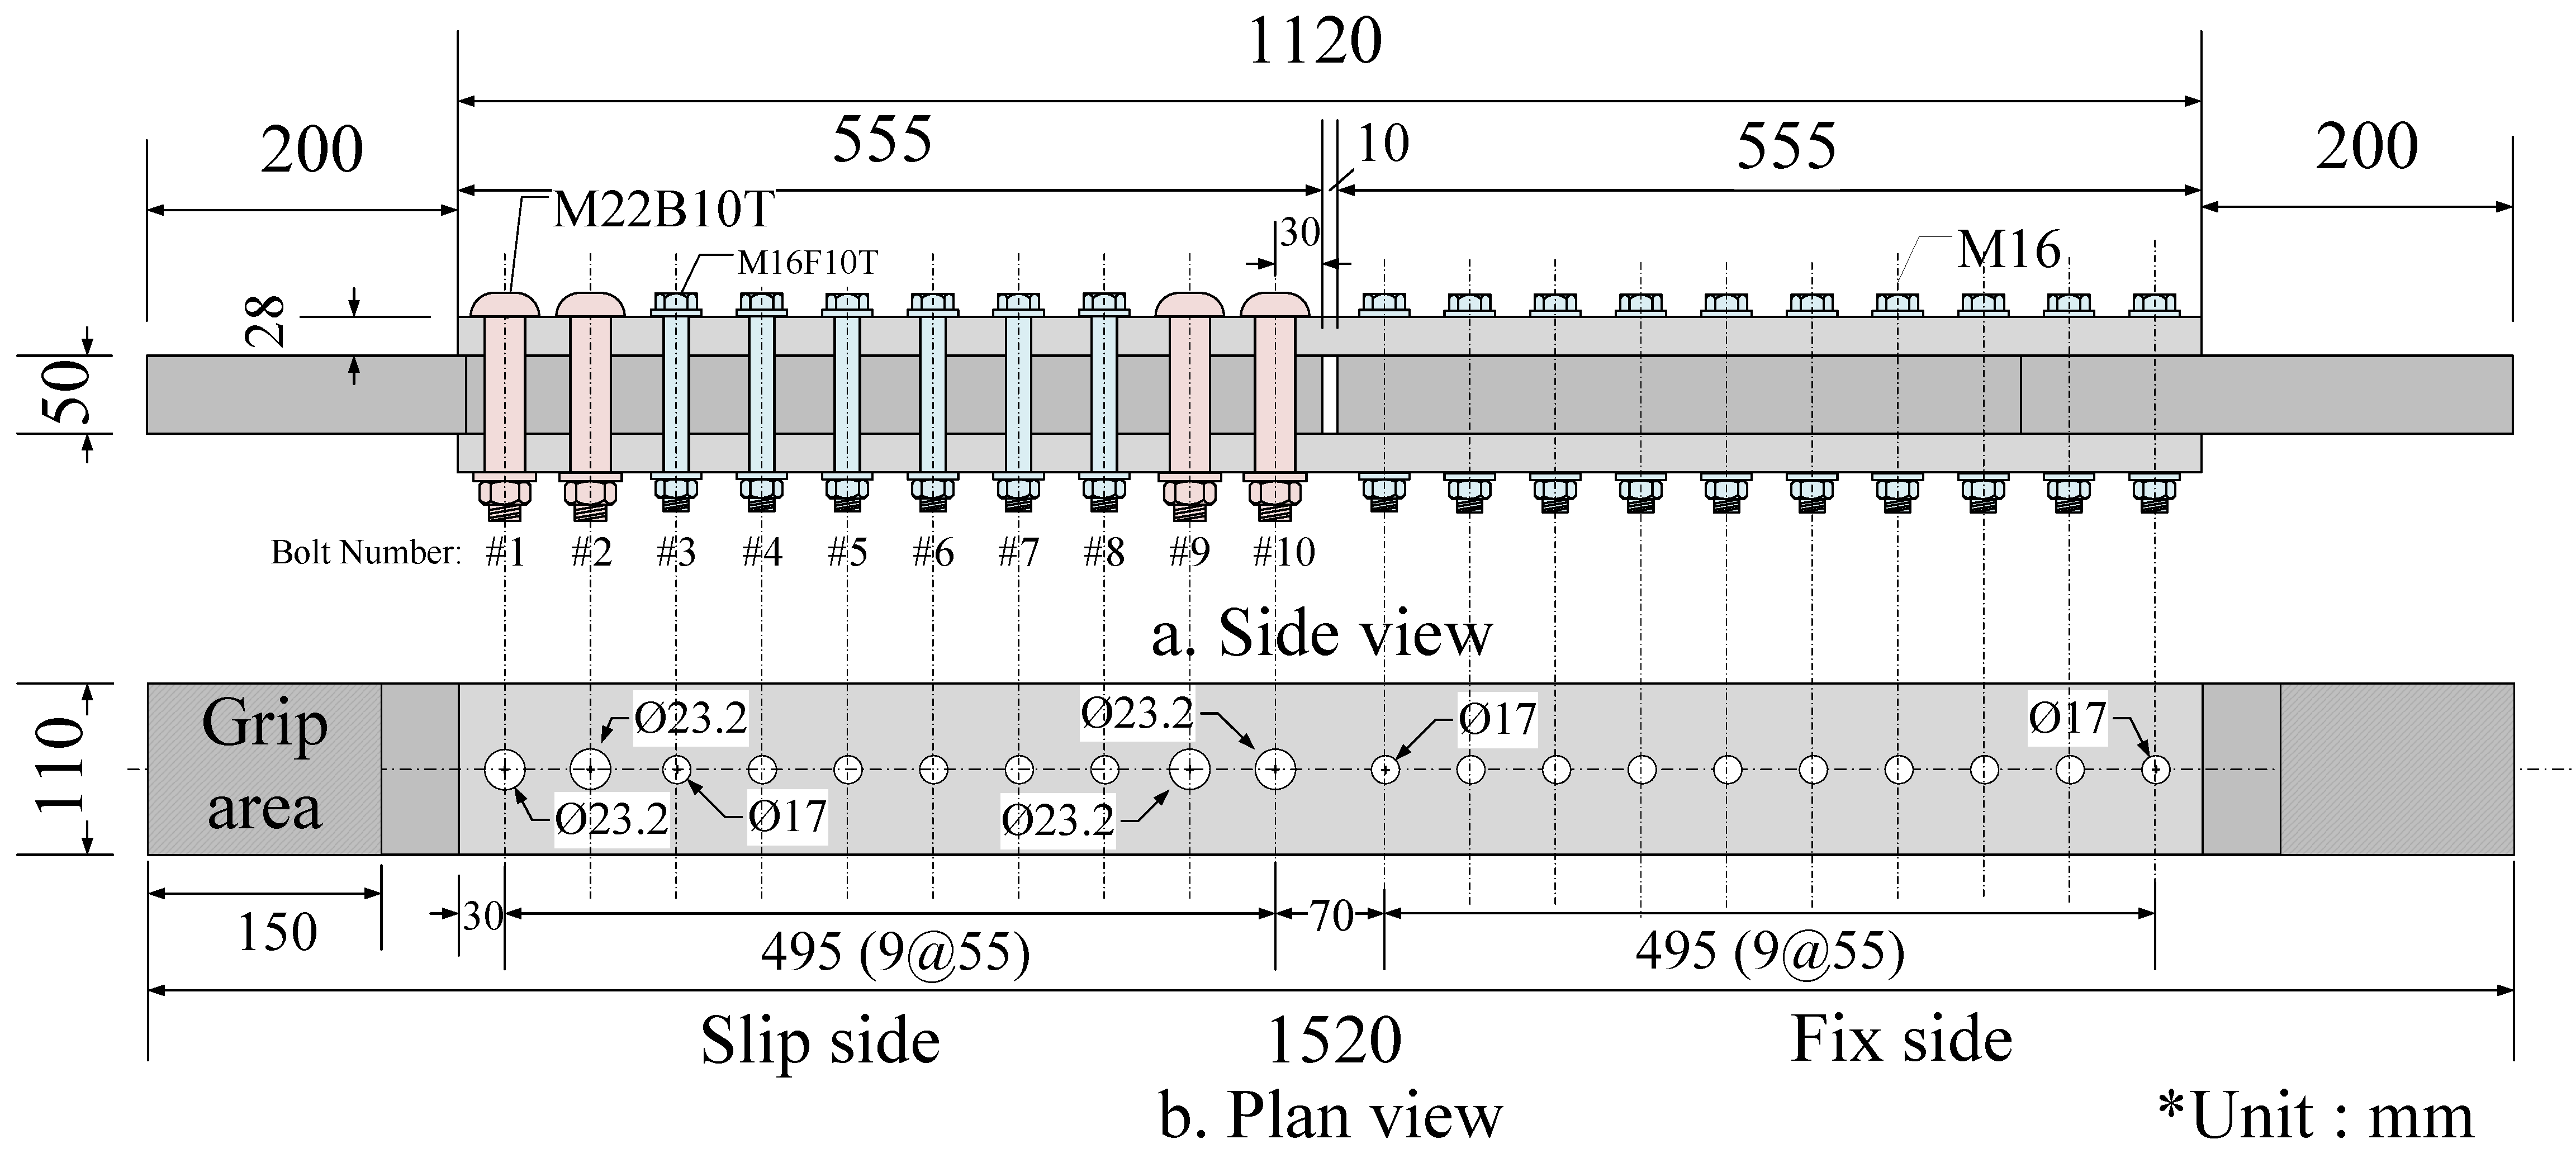
\includegraphics[width=\textwidth]{imgs/ch6/dimensions.pdf}
    \caption{Detailed dimensions of Hybrid joint}
    \label{fig-dimens}
\end{figure*}

\begin{figure}[htbp]
    \centering
    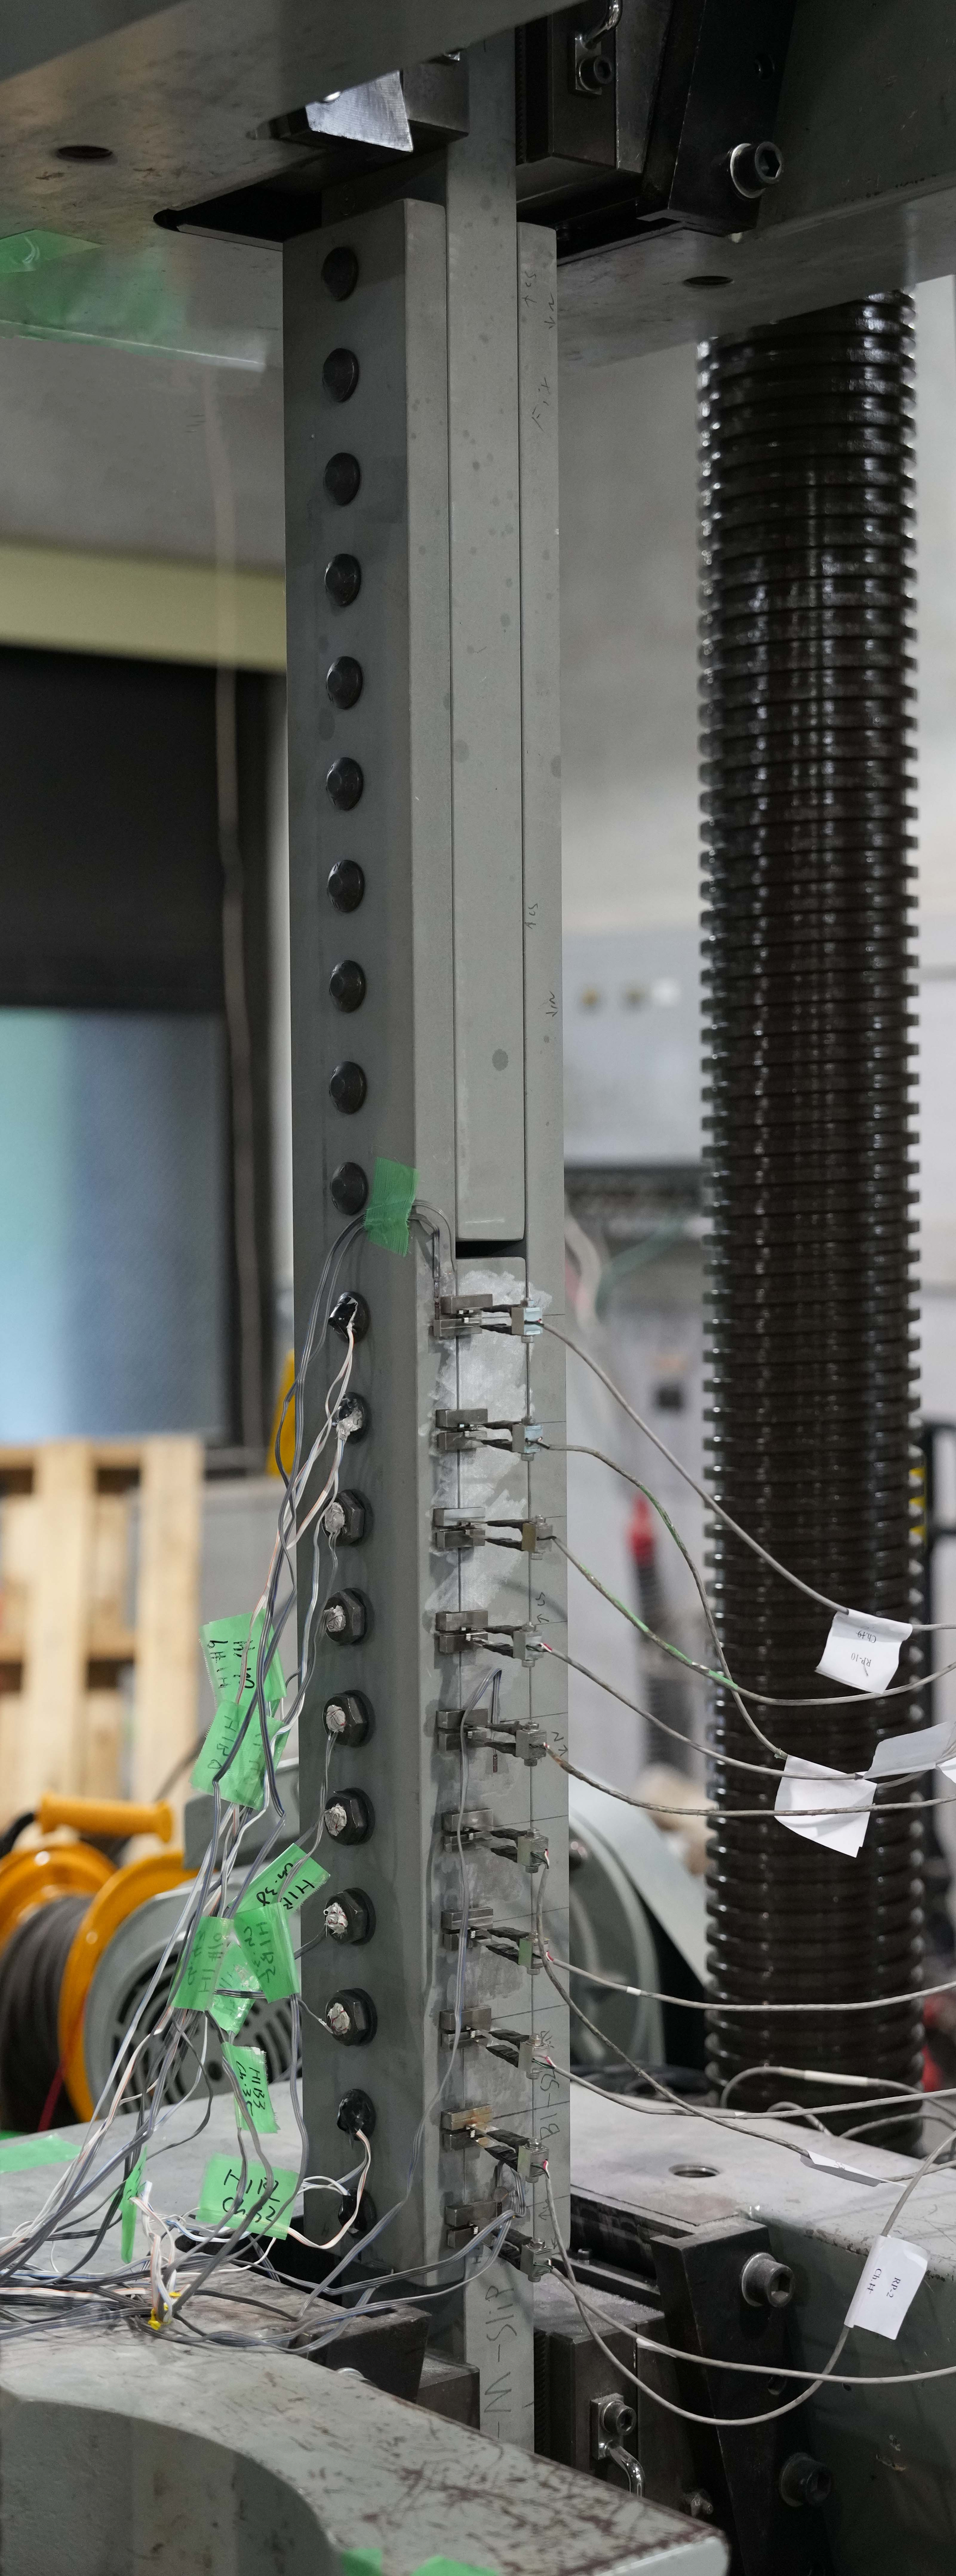
\includegraphics[width=0.25\textwidth]{imgs/ch6/set-up.jpg}
    \caption{Experiment Set-up}
    \label{fig-setup}
\end{figure}

\begin{figure*}
    \centering
    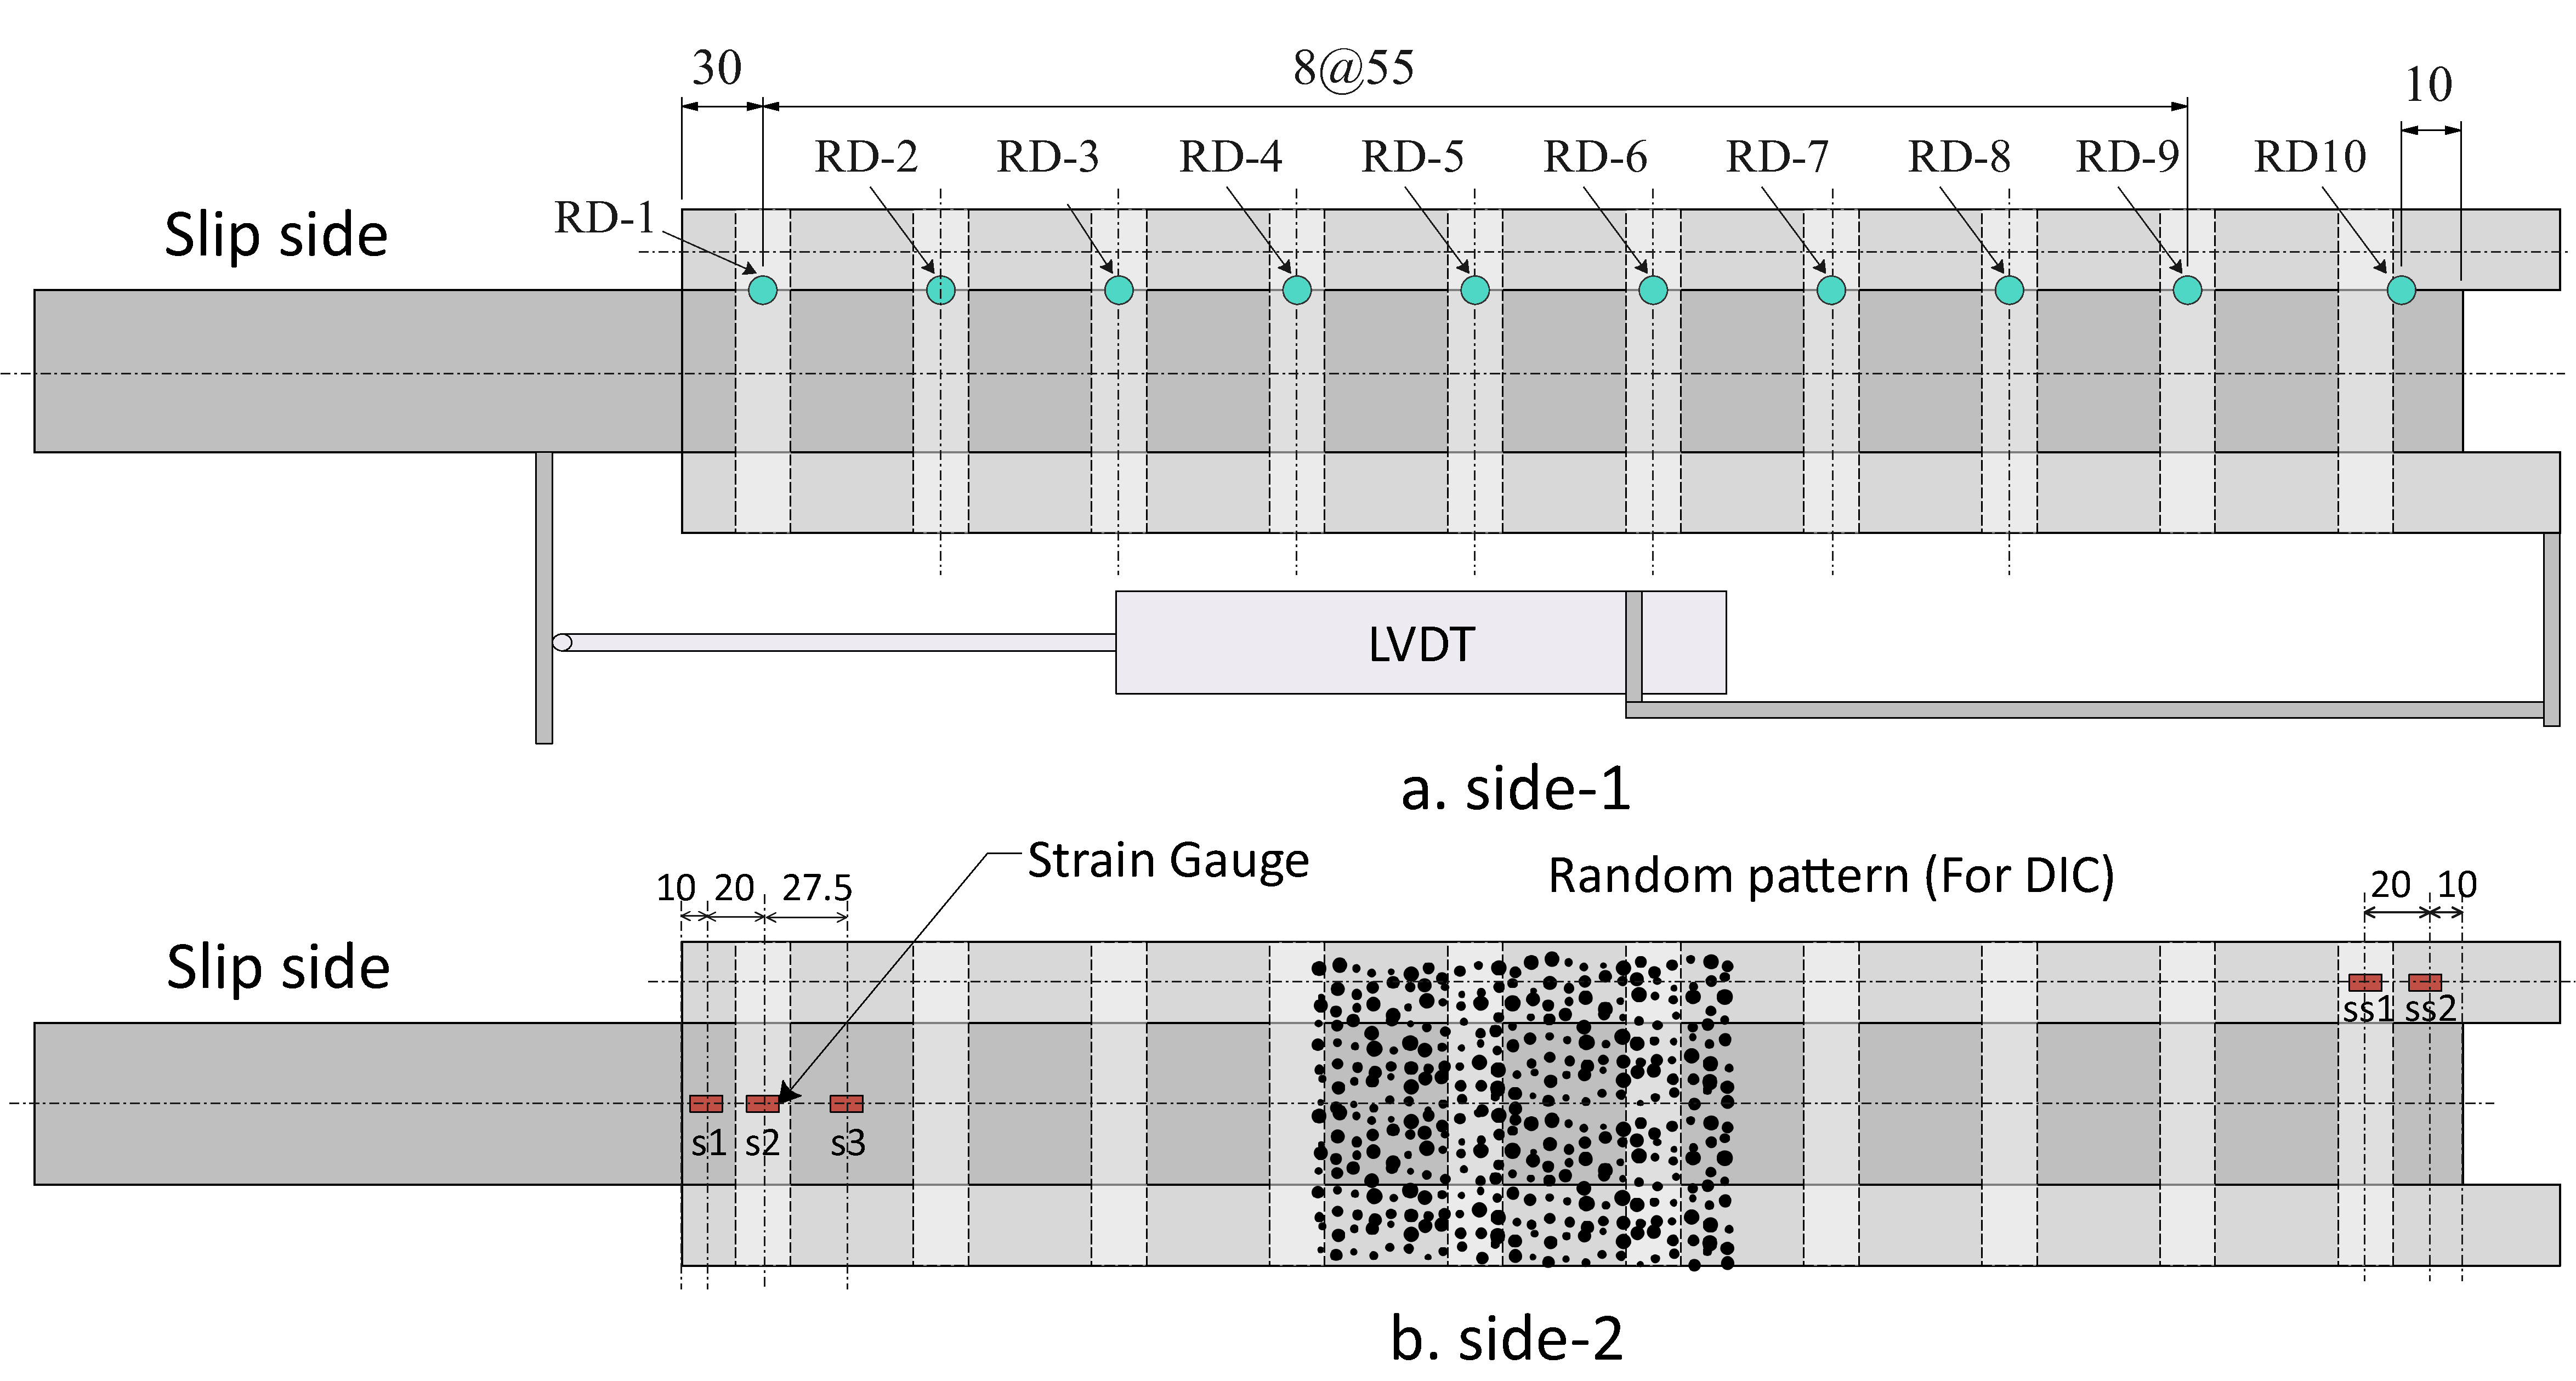
\includegraphics[width=0.9\textwidth]{imgs/ch6/mealoc.pdf}
    \caption{Measurement location (Unit: mm)}
    \label{fig-mealoc}
\end{figure*}

Interference fit bolts are installed using a hole with a diameter of 23.2mm. According to AASHTO \cite{AASHTO2020}, the common M16F10T bolt is installed using a 17mm diameter hole. Taking relaxation into account, the preload during installation for all bolts is 117kN \cite{douji2017}.

\subsection{Experimental cases}

The experimental specimens are shown in Table \ref{tab-expcase}. Previous research \cite{Chen2023MechanicalConnections} found that for long bolted joints with single columns of 8-12 rows, at least two or more Interference fit bolts should be used at each end of the joint to prevent excessive load sharing and premature shear yield of the bolts. Moreover, during the tightening process of the bolts, the bolt shank may undergo shrinkage caused by the Poisson's ratio effect, potentially leading to a loss of effectiveness in the interference fit. Therefore, in this experiment, the Hybrid case employs two Interference fit bolts at each end, whereas the Hybrid-NAF case means no preload for the interference fit bolt, which is only tightened to 5-10kN using a ratchet.

\begin{table*}[htbp]
\centering
\caption{ Experimental specimens }
\label{tab-expcase}
\begin{tabular}{@{}lcccccccccccc@{}}
\toprule
 \multirow{2}{*}{\begin{tabular}[c]{@{}c@{}} Specimens\end{tabular}} & \multicolumn{10}{c}{Fastener number (slip side)} & \multirow{2}{*}{\begin{tabular}[c]{@{}c@{}} Bolt \\ Preload\end{tabular}} \\ 
 \cmidrule(lr){2-11}
 &\multicolumn{1}{l}{\#1} & \multicolumn{1}{l}{\#2} & \multicolumn{1}{l}{\#3} & \multicolumn{1}{l}{\#4} & \multicolumn{1}{l}{\#5} & \multicolumn{1}{l}{\#6} & \multicolumn{1}{l}{\#7} & \multicolumn{1}{l}{\#8} & \multicolumn{1}{l}{\#9} & \multicolumn{1}{l}{\#10} &  \\ \midrule
Friction  &\faCircleO&\faCircleO&\faCircleO&\faCircleO&\faCircleO&\faCircleO&\faCircleO&\faCircleO&\faCircleO&\faCircleO& 117 \\
Hybrid & \faGear&\faGear&\faCircleO&\faCircleO&\faCircleO&\faCircleO&\faCircleO&\faCircleO&\faGear&\faGear& 117 \\
Hybrid-NAF & \faGear&\faGear&\faCircleO&\faCircleO&\faCircleO&\faCircleO&\faCircleO&\faCircleO&\faGear&\faGear& 5 --10 \\
\bottomrule
&&&&\multicolumn{9}{r}{\faCircleO : High-strength bolt, \faGear : Interference fit bolt}\\

\end{tabular}
\end{table*}


\section{Experiment Results}

\subsection{Installation of Interference fit bolt}
According to the regulations in Japan Road Association -- Japan Specifications For Highway Bridges - Part ii Steel Bridges\cite{douji2017} (hereinafter referred to as JSBH), the precision requirement for the bolt hole corresponding to the M22 bolt in bearing-type connections is 23.5±0.3mm. However, the maximum measured outer diameter of the Interference fit bolt shaft is 23.6mm. In order to confirm that the bolt can interference fit with the bolt hole after installation and fit tightly together, specimens with bolt hole diameters of 23.6mm, 23.5mm, and 23.2mm were respectively produced. Five interference fit bolts were randomly selected, and the average maximum  outer diameter of the bolt shaft (including the rib) measured with vernier calipers was 23.5 + 0.1mm.

The hole creation method involved drilling a pilot hole that is 1mm smaller than the target diameter, followed by enlarging the hole to the target diameter using a reamer. This approach guarantees that the bolt hole's accuracy is within ± 0.02mm.

The results showed that when the bolt hole is 23.6mm, the bolt can easily pass through the hole without achieving an interference fit. When the bolt hole is 23.5mm, it is not possible to insert the bolt into the hole by hand, but a hammer can be used with less force to install the bolt into the hole. When the bolt hole is 23.2mm, a significant amount of force is required to hammer the bolt into the hole.

Fig. \ref{fig-bcrossec} shows the cross-section of the bolt and the test plate. In both the 23.5mm and 23.2mm diameter holes, it can be observed that the ribs of the bolt have undergone plastic deformation, resulting in an interference fit. Fig. \ref{fig-bcrossec} reveals that the degree of deformation is more significant in the bolt shaft ribs and the hole wall of the test piece with the 23.2mm diameter hole. In order to achieve a better interference fit for the bolt, the diameter of the bolt hole for the Interference fit bolt used in this experiment was set to 23.2mm.


\begin{figure*}
\centering
\begin{subfigure}[t]{0.9\textwidth}
    \centering
    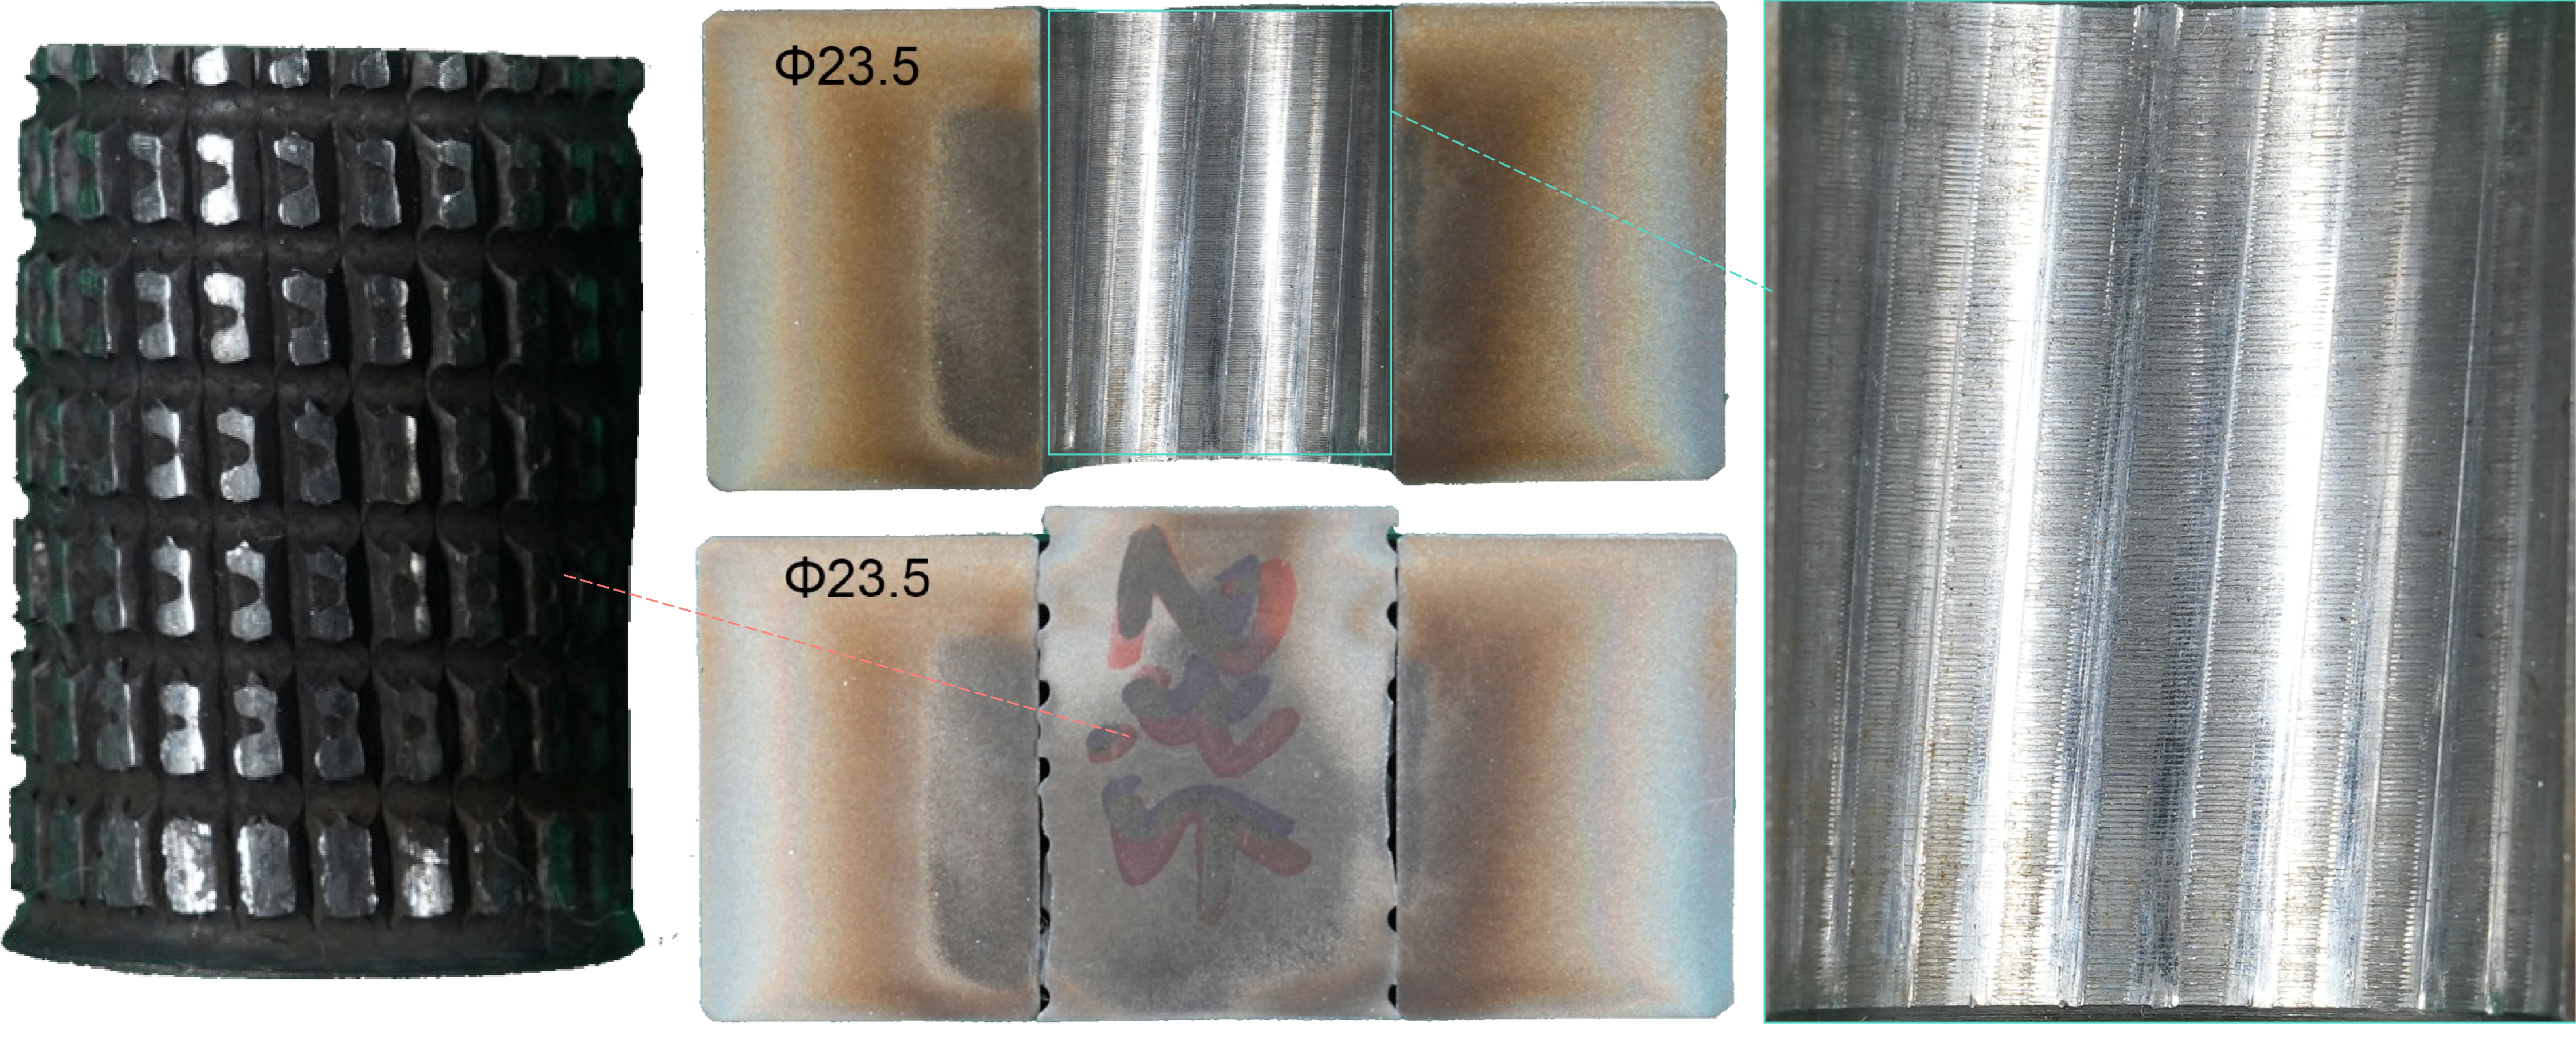
\includegraphics[width=\textwidth]{imgs/ch6/bstatus-23-5.pdf}
    \label{fig-bstatus235}
    \caption{23.5mm}
\end{subfigure}
\hfill
\begin{subfigure}[t]{0.9\textwidth}
    \centering
    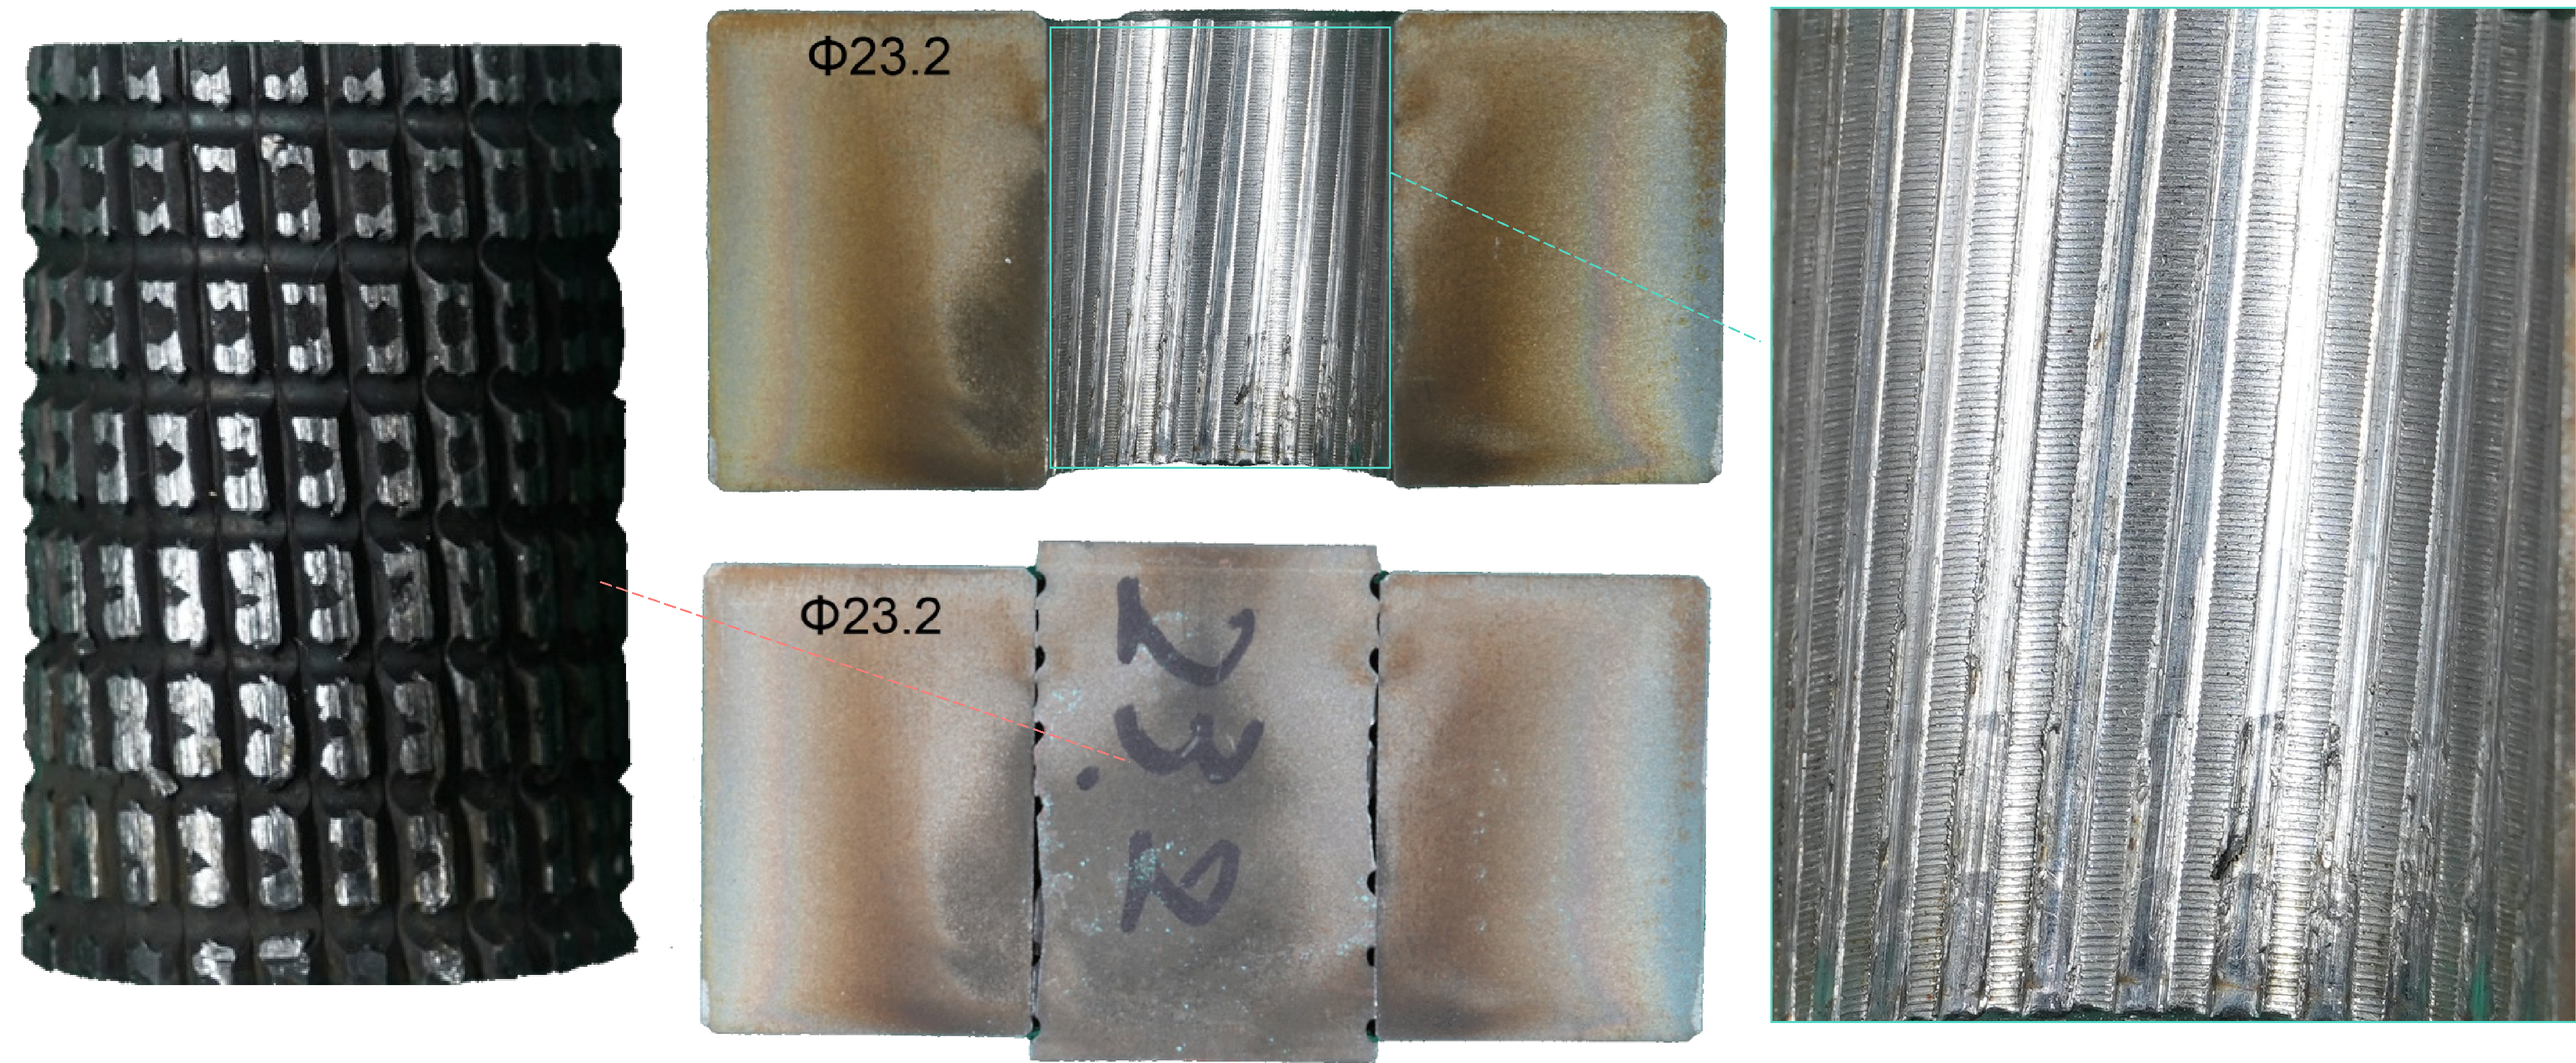
\includegraphics[width=\textwidth]{imgs/ch6/bstatus-23-2.pdf}
    \caption{23.2mm}
\end{subfigure}
\caption{The bearing status of the bolt shank and bolt hole.}
\label{fig-bcrossec}
\end{figure*}


\subsection{Deformation and relative displacement}

Fig. \ref{fig-loaddisp} shows the relationship between the load and the whole deformation of the joint. Clear slippage occurred at the friction type joint at 1361 kN, with the load decreasing to approximately 1048 kN (a change rate of approximately 23\%). The overall deformation of the joint increased from 3.7 mm to 6.5 mm, (a change rate of approximately 75\%). For the hybrid joint, slippage occurred when the load reached 1456 kN, and the load decreased from 1456 to 1407 kN (a change rate of approximately 3\%). As for the joint deformation, it decreased from 3.955 mm to 3.989 mm (a change rate of only approximately 0.8\%). The overall load-deformation relationship of the hybrid joint remains quasi-linear up to the upper load limit of 1800 kN, although a minor amount of slip occurs, and there have only 1mm minor residual deformation. In addition, for the Hybrid-NAF case, compare to the hybrid case besides a slight decrease in the initial slope and a minor reduction in the slippage load, the trend of the curve is not significantly different.

Fig. \ref{fig-rd10} shows the relationship between load and relative displacement at a distance of 10 mm from the end of main plate(CDT-6). Similar to the overall deformation figure, significant slippage occurred at the friction joint, with relative displacement increasing from 0.163 to 1.632 (an increase of approximately 900\%). As for the hybrid joint, the relative displacement increased from 0.184 to 0.342 (an increase of approximately 85\%). The hybrid joint exhibits a small amount of slippage similar to the results of previous studies\cite{kamei2010} on experiment of individual interference-fit bolts. This is due to the existence of small clearance between the bolt hole wall and the rib of the Interference fit bolt, resulting in inevitable slight slippage. The slip load of hybrid joints is 7\% higher than that of friction joint joints.

The value of slip load reduction and the slippage was summarized in Table \ref{tab-sumld}.

\begin{figure}[htbp]
\centering
    \begin{subfigure}[t]{0.45\textwidth}
        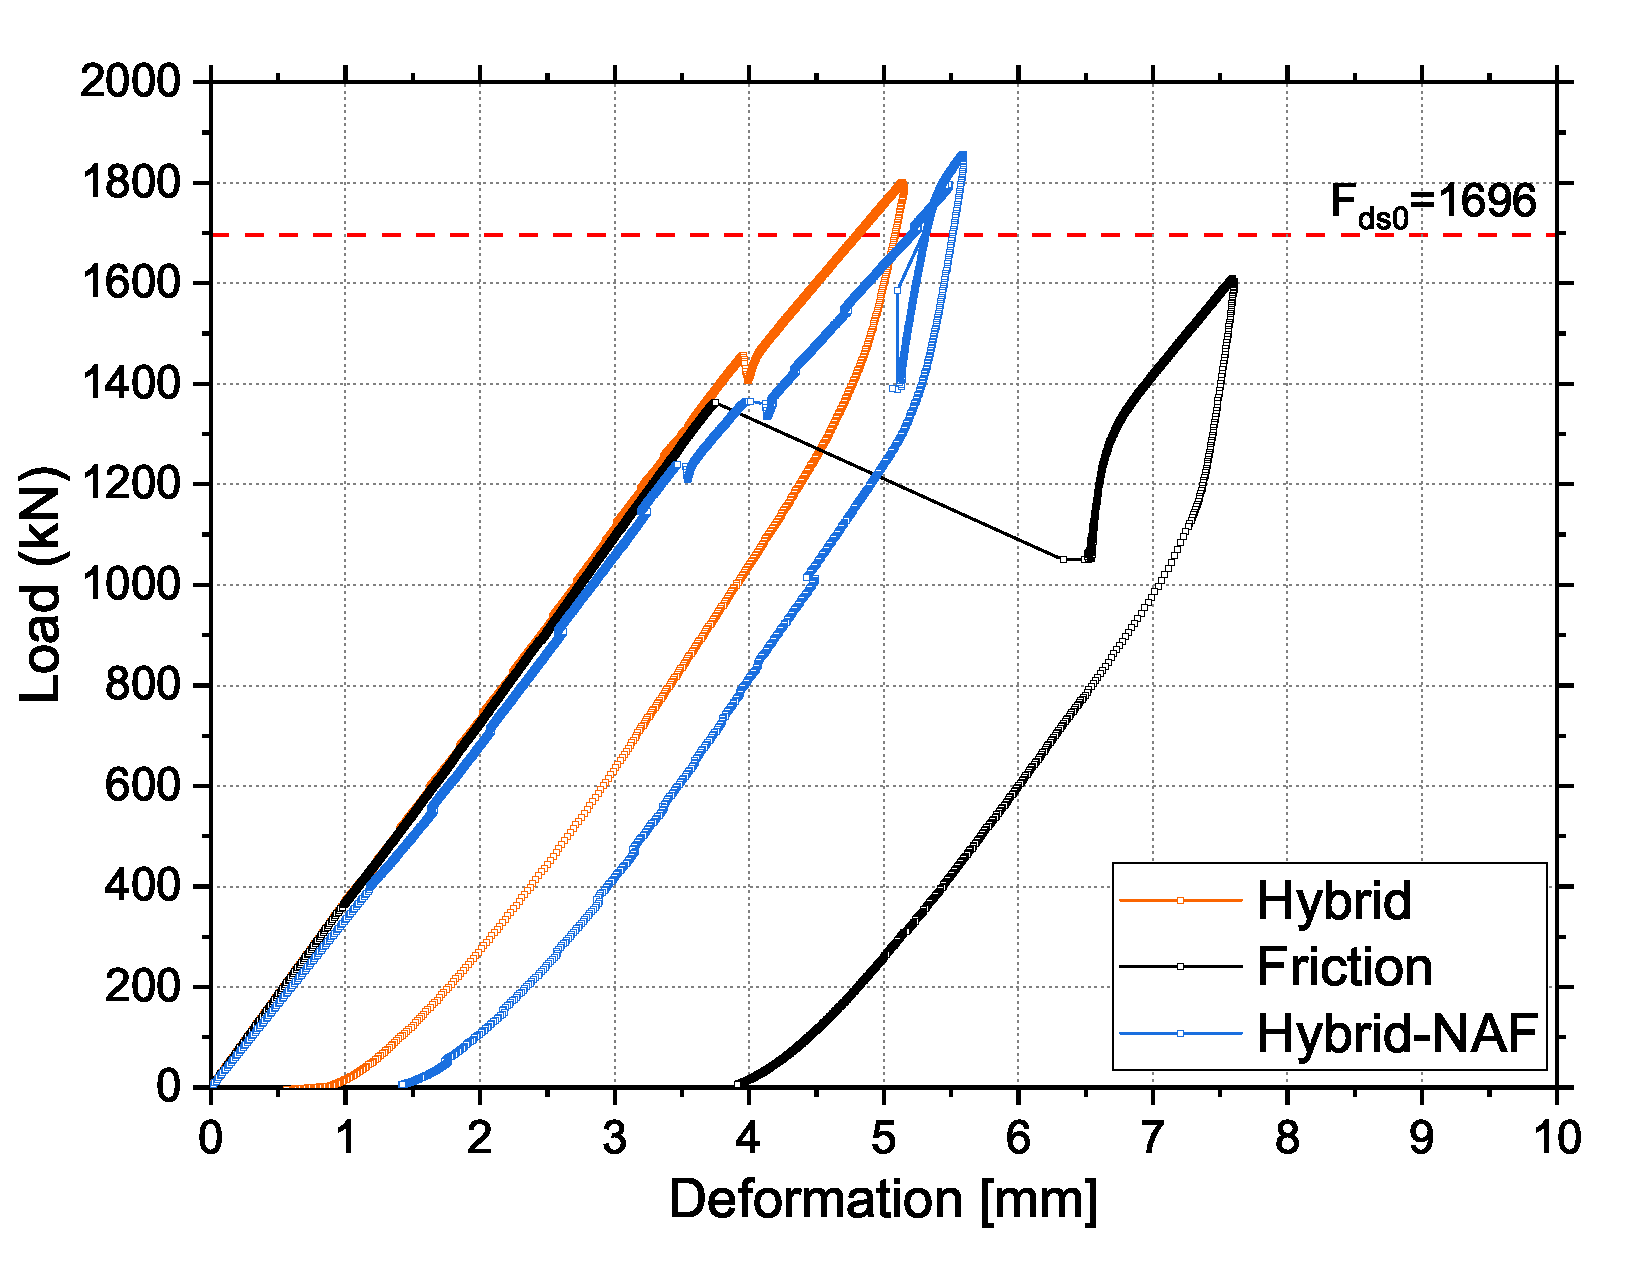
\includegraphics[width=\linewidth]{imgs/ch6/load-disp-cor.eps}
        \caption{Deformation}
        \label{fig-loaddisp}
    \end{subfigure}
    \hfill
    \begin{subfigure}[t]{0.45\textwidth}
        \includegraphics[width=\linewidth]{imgs/ch6/RD-bolt10.eps}
        \caption{Relative displacement}
        \label{fig-rd10}
    \end{subfigure}
    \caption{Relationship between load and deformation or relative displacement}
    \label{fig-disp}
\end{figure}


\begin{table}[]
\centering
\caption{ Summary of load drop and slip }
\label{tab-sumld}
\begin{tabular}{@{}ccccc@{}}
\toprule
Case & Slip Begins & End of Slip & Difference & Rate of Change \\ \midrule
\multicolumn{5}{c}{Load {[}kN{]}} \\
Friction & 1361 & 1048 & -313 & -23\% \\
Hybrid & 1456 & 1407 & -49 & -3\% \\
Hybrid-NAF & 1238 & 1210 & -28 & -2.2\% \\
\multicolumn{5}{c}{Deformation {[}mm{]}} \\
Friction & 3.7 & 6.5 & 2.8 & +75\% \\
Hybrid & 3.955 & 3.989 & 0.034 & +0.8\% \\
Hybrid-NAF & 3.46 & 3.54 & 0.08 & +2.3\% \\
\multicolumn{5}{c}{Relative Displacement {[}mm{]}} \\
Friction & 0.163 & 1.632 & 1.469 & +901\% \\
Hybrid & 0.184 & 0.342 & 0.158 & +85\% \\ 
Hybrid-NAF & 0.146 & 0.327 & 0.181 & +124\% \\ 
\bottomrule
\end{tabular}
\end{table}




\subsection{Bolt preload}

Fig. \ref{fig-laf} shows the relationship between bolt preload reduction ratio and load of each bolt, the bolt preload reduction ratio is calculated by $N/N_0$, where $N$ is real-time bolt preload, and $N_0$ is the bolt preload before loading. 

For the Friction joint, the most significant decrease in bolt preload occurred on bolt \#10, where the preload dropped to about 90\% when slip occurred (1361kN) as shown in Fig. \ref{fig-laff}. This is a 5\% difference compared to bolt \#6, which had the smallest decrease in preload.  The main reason for the significant reduction in preload at bolt \#10 is that the deformation of the splice plate at bolt \#10 is greater than that of the main plate at bolt \#1. Although the main plate had a larger net cross-sectional than the splice plate, considering the 1.1 times stress enhancement due to friction on the net cross-section of the main plate, the stress at the net cross-section of the splice plate would be almost the same as the main plate when subjected to the same tension. Moreover, it was found that the direct strain at bolt \# 10 of splice plate is greater than the strain at bolt \# 1 of main plate. Furthermore, apart from bolt \# 1, the preload of the other bolts have not decreased uniformly, with an approximate variation of 2\%. After 1361 kN was reached, a severe impact occurred due to the large slip that occurred in the joint and the momentary transition of the joint from a sliding to a bearing state, as a result, all strain gauges on the bolts were damaged and it was not possible to obtain bolt preload data.

For the hybrid joint as shown in Fig. \ref{fig-lafhy} , an observation was made that, at the load of 1361kN, there was a uniform distribution of bolt reduction ratio with a variation of around 1\% when compared to the friction type joint. Although we did not measure preload for the interference fit bolt, based on the data from HSB, we posit that the hybrid joint's load distribution is more uniform in comparison to the friction joint. Moreover, in the event that slip occurs at the joint, the variance of each bolt's preload is not significant, even after reaching 1456kN. When load reached 1800kN, the maximum reduction ratio in preload variation is only 6\%. Therefore, it can be considered that the load distribution of hybrid joints is more uniform and the load transmission is smoother than that of friction joints.

\begin{figure}[htbp]
    \centering
    \begin{subfigure}[t]{0.7\textwidth}
    \centering
    \includegraphics[width=\linewidth]{imgs/ch6/loadaf-fric.eps}
    \caption{Friction type joint }
    \label{fig-laff}
    \end{subfigure}
    %\vspace{1cm}
    \begin{subfigure}[t]{0.7\textwidth}
    \centering
    \includegraphics[width=\linewidth]{imgs/ch6/loadaf-hyb.eps}
    \caption{Hybrid joint }
    \label{fig-lafhy}
    \end{subfigure}
    \caption{The relationship between Bolt preload reduction ratio and load of each bolt. [\%]}
    \label{fig-laf}
\end{figure}

\subsection{Distribution of relative displacement}

The Distribution of relative displacement (When load = 0.8$F_{sf}$ = 1088kN, while $F_{sf}$ is Friction type joint slip load) is as shown in Fig. \ref{fig-rdbar}. Green bar represents the friction joint and the orange bar represents the hybrid joint. For the positions RD-1 and RD-2 at the ends of the joint, the relative displacement of the hybrid joint is significantly lower in comparison to the friction type joint. This low relative displacement can be attributed to the interference fit of the bolts \# 1 and \# 2, making it more difficult to generate relative displacement when the elastic slip stage is nearing its end. However, at the other end of the hybrid joint, at interference fit bolts \# 9 and \# 10, the relative displacement at RD8, 9 and 10 is actually higher than that of the friction type joint.It is speculated that the higher relative displacement observed at bolts \#9 and \#10 may be attributed to a suboptimal interference fit.

In addition, the hybrid joint has a more uniform distribution of relative displacement compared to the friction joint. This finding is consistent with the results discussed in section 3.3 regarding the distribution of bolt preload reduction. As a result, it can be inferred that the hybrid joint demonstrates a more uniform load distribution mechanism. The load sharing mechanism discussed in this paper is also similar to the analytical discussions found in previous studies \cite{Chen2023MechanicalConnections}.

\begin{figure}[htbp]
    \centering
    \includegraphics[width=0.6\textwidth]{imgs/ch6/RD-bar.eps}
    \caption{Distribution of Relative displacement (When load = 0.8$F_{sf}$ = 1088kN, while $F_{sf}$ is Friction type joint slip load) }
    \label{fig-rdbar}
\end{figure}

\subsection{Strain of the plate}

The Relationship between Load and strain are shown in Fig. \ref{fig-LS}, Where the measurement position are shown in Fig. \ref{fig-mealoc}. Fig. \ref{fig-s1ss2} shows the S1 and SS2 strain of the end of friction type joint, it is evident that the strain SS2 on the inner side of the splice plate has a steeper slope than S1 of the main plate. This indicates that the inner side of the splice plate undergoes a greater deformation in the tensile direction (referred to as the y-direction) compared to the main plate under the same load. Consequently, the deformation ($0.3\delta_y$) of the splice plate perpendicular to the tensile direction (x-direction) also increases. The deformation of the splice plate in the x-direction (i.e. the reduction in thickness) directly leads to a decrease in the bolt preload. This is because the deformation of the main plate at S1 is suppressed and part of the load is transferred to the splice plate by interfacial friction, causing the deformation of the splice plate at SS2 to be slightly greater than that of the main plate at S1. This also explains why the bolt preload decreased faster for the inner bolt \# 10 than for the outer bolt \# 1.

Compared to the friction joint, the hybrid joint exhibited higher slope of direct strain S1 and load. At 1456 kN, there was a minor slip, resulting in a slight change in slope. However, the strain remained quasi-linear until reaching the maximum load of 1800 kN. In contrast, for the friction joint, non-linear behavior was observed at around 800 kN, possibly due to uneven load distribution, reaching the limit of the end bolts' slip resistance. Due to the reduction in bolt preload, the slip resistance capacity decreases as the load increases until slip occurs.

Furthermore, focus on direct strain at position S3 that has already transmitted a portion of the load through bolt \# 1; this non-linear behavior becomes more evident and there is some residual strain after unloading. Nevertheless, there is no discernible non-linear behavior in the hybrid joint. The slop decreases only slightly during slip and after unloading, remains linear without the presence of residual strain. It can be inferred that the load-strain relationship of the hybrid joint is quasi-linear overall (up to the maximum load of 1800kN).

\begin{figure}[htbp]
\centering
    \begin{subfigure}[t]{0.6\textwidth}
        \includegraphics[width=\linewidth]{imgs/ch6/S1SS2-F.eps}
        \caption{S1,and SS2 for Friction type joint}
        \label{fig-s1ss2}
    \end{subfigure}
    \hfill
    \begin{subfigure}[t]{0.6\textwidth}
        \includegraphics[width=\linewidth]{imgs/ch6/S3-FH.eps}
        \caption{s1 and s3 for Friction and Hybrid joint}
        \label{fig-s3FH}
    \end{subfigure}
    \caption{Relationship between Load and Direct Strain}
    \label{fig-LS}
\end{figure}

\section{Discussion}

\subsection{Cross-section observation after slipping}

Fig. \ref{fig-csob} shows the Cross-section of Hybrid joint. The cross-sectional diagram was obtained from the hybrid joint that underwent a load of up to 1800kN. Fig. \ref{fig-csob1} shows the cross-sectional diagram of bolts \#1 - \# 3, revealing that the deformation of the rib on the non-bearing side is very small as observed in the magnified portion of bolt \#1 on the right side. Likewise, the magnified section of Bolt \#2 on the opposite side of the bearing suggests minor deformation of the rib. It appears that some ribs do not make contact with the hole wall when the interference fit bolt is hammered into the hole. Consequently, the desired interference fit is not produced, resulting in a minor slip in the joint. This slip is believed to be caused by the clearance created during the bolt installation, as well as slight plastic deformation of the rib.

\begin{figure*}
    \centering
    \begin{subfigure}[t]{0.85\textwidth}
    \centering
    \includegraphics[width=\linewidth]{imgs/ch6/cros-sec-ob1.pdf}
    \caption{Bolt \#1 -- \#3}
    \label{fig-csob1}
    \end{subfigure}
    %\vspace{1cm}
    \begin{subfigure}[t]{0.85\textwidth}
    \centering
    \includegraphics[width=\linewidth]{imgs/ch6/cros-sec-ob2.pdf}
    \caption{Bolt \#4 -- \#6}
    \label{fig-csob2}
    \end{subfigure}
    \caption{Cross-section of Hybrid joint's each bolt, Loading to 1800kN}
    \label{fig-csob}
\end{figure*}


Fig. \ref{fig-dicdisp} shows the displacement of the hybrid joint case at a load of 200kN, measured by DIC methods, taken from the side of the joint. It was found that the displacement on the nut side of the joint (i.e. SP2 side) is greater than the displacement on the bolt head side (i.e. SP1 side). This observation is consistent with the results obtained from cross-sectional observations. Insufficient interference fit resulted in an increase in displacement and a slight occurrence of slippage.

\begin{figure*}
    \centering
    \includegraphics[width=0.85\linewidth]{imgs/ch6/dic-B3-200kN.pdf}
    \caption{Displacements of hybrid joint when load is 200kN }
    \label{fig-dicdisp}
\end{figure*}

\subsection{Load reduction for long bolted joint}

The European Convention for Constructional Steelwork (ECCS), and ISO/TC specify that the resistance should be reduced by a factor of $\beta_{rd}$ when the spacing between the first and last bolt in a joint is larger than 15d as shown in Eq.\ref{eq-eurolon} \cite{eccs1985,isohtb}. AASHTO \cite{AASHTO2020} provides the nominal shear resistance of bolts in joints longer than 38.0 in. must be reduced by an additional factor of 0.83 or 0.75/0.9\par

\begin{equation}\label{eq-eurolon}
    \beta_{rd} = 
    \begin{cases}
    1 & (L \leq 15 d) \\ 
    1.08-L / (200 d) & (15 d < L \leq 65 d)\\ 
    0.75 & (65 d < L)
    \end{cases}
\end{equation}

Eurocode 3 (EN 1993-1-8:2005) \cite{eurocode3-21} provisions that where the distance $L_j$ between the centers of the end fasteners in a joint, measured in the direction of force transfer is more than 15d, the design shear resistance of all the fasteners should be reduced by multiplying it by a reduction factor $\beta_{Lf}$:
\begin{equation}
    \beta_{Lf}=1-\frac{L_j - 15d}{200d}
\end{equation}

Japanease Specification for Highway Bridge (JSHB) \cite{douji2017} published by Japan Road Association states that when the number of row exceeds 8 in bolted joint, a reduction factor must be applied to the slip resistance, as shown in Table \ref{ch6tab-jpredu}.
\begin{table}[h]
    \centering
    \caption{Reduction of slip resistance of bolted joint of JSHB-JRA}
    \begin{tabular}{cccccc}
    \toprule
        Number of Row &  8 & 9 & 10 & 11 & 12 \\ \midrule
        Reduction factor & 1.00 & 0.98 & 0.96 & 0.94 & 0.92 \\ \bottomrule
    \end{tabular}
    \label{ch6tab-jpredu}
\end{table}

Furthermore, due to the non-uniformity of load distribution, the bolts are unable to fracture simultaneously, consequently leading to a reduction in the ultimate limit bearing capacity.\cite{Takai2021BoltUnbuttoning,Peng2013FeaDimensions,peng2010}.

Table \ref{tab-rera} presents the experimentally acquired slip loads $P_{s}$ of each case, along with their corresponding calculated slip resistance $F_{ds}$. It also shows the load reduction rate between the experimentally acquired slip loads $P_{s}$ and the calculated values $F_{ds}$. Eurocode 3 \cite{eurocode3-21} recommend that interference fit bolts should be designed by calculating slip resistance in the same way as HSB friction type connection. Slip resistance $F_{ds}$ is calculated from Equation \ref{eq-fds1ch6} and slip load $P_s$ is the load when the first load drop occurred. The lengths of the Friction and Hybrid joint $L_j$ are both 495 mm (where $L_j$ is the distance between the centres of the end fasteners in a joint). The load reduction rate of the friction type reaches 0.79, which is lower than the values specified by Eurocode (calculated to be 0.92) and JHSB (calculated to be 0.96). It is inferred that this is due to the use of thick plate (50mm in main plate) in this experiment. Because the thick plate causes the bearing stress on the bolt to be uneven, the bolt will be more susceptible to bending deformation, resulting in loss of preload. While the Hybrid joints have a slip load reduction of 0.9, which is about 10\% higher than friction joints. The slip resistance reduction ratio for the hybrid joint without preload (Hybrid-NAF case) on the interference fit bolts was 0.92, which is approximately the same as for the hybrid joint. This is because regardless of the presence of preload in the interference fit bolt, the amount of slip until the load is increased is nearly the same for both cases. This depends on the gap in the bolt and hole wall and the plastic deformation of the rib. 



\begin{table}[]
\centering
\caption{Slip resistance reduction ratio of each case}
\begin{tabular}{@{}lccc@{}}
\toprule
 & \begin{tabular}[c]{@{}c@{}}Slip load $P_s$\\ kN\end{tabular} & \begin{tabular}[c]{@{}c@{}}slip resistance $F_{ds}$\\ kN\end{tabular} & load reduction rate \\ \midrule
Hybrid & 1456 & 1618 & 0.90 \\
Hybrid-NAF & 1237 & 1341 & 0.91 \\
Friction & 1362 & 1726 & 0.79 \\ \bottomrule
\end{tabular}
\label{tab-rera}
\end{table}

\begin{equation}
    \label{eq-fds1ch6}
    F_{ds} = \sum_n \mu \times N_0 \times m
\end{equation}

where $\mu$ is the slip coefficient = 0.8 taken from the slip factor test which arranged two bolts and has the same plate thickness and the same faying surface condition as this test, $N_0$ is the preload of the bolts before loading, $m$ is the number of shear planes, $n$ is the number of the bolt.


In addition, the theoretical calculations indicate that applying a preload of 106kN to a bolt with a diameter of 22mm would result in a contraction of 0.009 mm, which is much smaller than the manufacturing tolerances of the bolt hole or the bolt shank diameter. Therefore, the horizontal shrinkage of the bolt shaft is small enough to be negligible.

Bolt shaft shrinking value ($\Delta d$) is:
\begin{equation}
    \label{eq-bdefo}
    \Delta d=\delta_{yb}d_{ib}=\frac{N_0v}{EA}d
\end{equation}
where $\delta_{yb}$ is the bolt strain of y-direction (axial direction), $d_{ib}$ is the diameter of the interference fit bolt, $A_{ib}$ is the cross-sectional area of the interference fit bolt shaft.

Therefore, result as the amount of bolt preload does not have a significant effect on the slip behavior, and it can be considered that the reduction of slip load is related to the bearing capacity of the rib, as insufficient contact area of the rib results in excessive contact pressure and compression plastic deformation. 

\begin{figure}[htbp]
    \centering
    \includegraphics[width=0.6\textwidth]{imgs/ch6/nor-load-disp.eps}
    \caption{The relationship between normalised load and normalised deformation. (Normalised load is the load divided by the sliding load $F_s$, and normalised deformation is the deformation divided by the joint length $L_j$).}
    \label{fig-ldnor}
\end{figure}

Fig. \ref{fig-ldnor} shows the relationship between normalised load and normalised deformation. It can be seen that the initial slop is higher for the Hybrid-NAF case, this is due to the bearing resistance of the interference fit bolts is not included in the calculation of the slip resistance, comparing this with the behaviour of the friction joint, it can be confirmed that the bearing resistance is included in the load sharing of the Hybrid-NAF joint result a high initial slope of Hybrid-NAF case, despite the minor amount of slip that occurs. The minor amount of slip is due to the inadequacy of the interference fit,  which results in the interference fit bolt in not being able to fully resist the portion of the load lost as a result of the slip that occurs. 


\subsection{Limit state}

Previous study \cite{fisher1965behavior} shows that load will firstly transmit by the connection with higher stiffness, and the bearing-type connection will only play a significant role in load sharing when the friction-type connection approaches its limit. Therefore, the limit state of a hybrid joint relies on the state of the bearing type connection, which can manifest as either the shear yield limit of the bolt or the bearing deformation limit of the main plate.

This study considers that for hybrid joints using bearing type bolted connections and friction connections together, the design under the serviceability limit state can be performed by accumulating the bearing resistance of interference fit bolt and the slip resistance of HSB.

However, in this experiment, slight slippage occurred in the hybrid joint, which was believed to be caused by the gaps between the rib and the hole wall. Therefore, regarding the definition of the limit state of the hybrid joint, by referring to the Japanese AIJ Recommendations for Design of Connections in Steel Structures \cite{2012AIJStructures}, a slip limit of 0.2mm can be set for the joint. The maximum load within a relative slip coefficient of 0.2mm is taken as the serviceability limit state, which is the slip resistance $F_{ds}$ in Table \ref{tab-rera}. Since a slight slip occurred in the hybrid joint in this experiment, the behavior after 0.2 mm cannot be determined based on this data. 

Despite this, hybrid joints in the slip limit state exhibit greater strength compared to friction joints. The load distribution is also more even and the relative displacement of the ends is smaller. Consequently, the performance of hybrid joints is superior to that of existing friction joints under the current slip limit specification, and the study concludes that designing hybrid joints under the current slip limit specification is feasible.

\section{Summarize}

This study focuses on interference fit bolts assembled at both ends of friction type bolted joint to elucidate the slip resistance and deformation of the hybrid joints, and to verify whether the interference fit bolts can be assembled in the friction type joints to improve the strength of the joint. Tensile tests were performed with three specimens: friction type bolted joint, hybrid joint, and hybrid joint with non-preload interference fit bolts. 

On the basis of the results of our investigation, we have made the following findings and conclusions. \par

\begin{enumerate}

\item The slip load of a 10-row hybrid joint assembled with four interference fit bolts at both ends is approximately 7\% higher than that of a friction-type joint. If the initial preload of the bolts is considered inconsistent, the result of dividing the slip load by the corresponding calculated slip resistance is approximately 10\% higher for the hybrid joint than that for the friction-type joint.

\item The distributions of relative displacements and reduction in the preload on the individual bolts of the joint show that the hybrid joint has a small dispersion of the data when compared with the friction-type joint, suggesting that the uneven load distribution and deformation of the joint can be improved by installing interference fit bolts. This allows the inner bolts of the hybrid joint to share a greater part of the load than the friction-type joint for the same load level, thus reducing the load concentration on the outer bolts. The deformation of the hybrid joint improves owing to the considerable reduction in the outermost relative displacement RD1. The performance of hybrid joints is superior to that of the existing friction-type joints under the current slip limit specification. 

\item The overall load--deformation relationship of the hybrid joint remains quasi-linear up to the upper load limit of 1800 kN, although a minor amount of slip occurs. Moreover, the total residual deformation of the hybrid joint is only 0.2\% relative to the length $L_j$ of the joint. In contrast, the friction-type bolted joint produces a residual deformation of 0.75\% when loaded to 1600 kN. Therefore, within the quasi-linear range, it can be expected that the hybrid joint will have a high serviceability limit strength.

\item The observation of the cross section showed that the rib portion of the interference fit bolt tail did not provide a good interference fit (the rib was not in contact with the hole wall or the contact area was too small). This resulted in the interference fit bolt being unable to fully resist the portion of load lost due to the slip, causing a minor slip to occur. This is also illustrated by the fact that the displacement of the splice plate SP2 on the nut side is greater than that of the splice plate SP1 on the head side of the bolt.


\end{enumerate}
\chapter{Limit state design methods of Hybrid Connection}
\label{ch7}

%%%%%%%%%%%%%%%%%%%%%%%%%%%%%%%%%%%%%%%
% IMPORTANT
\begin{spacing}{1.25} %THESE FOUR
\minitoc % LINES MUST APPEAR IN
\end{spacing} % EVERY
\onehalfspacing % CHAPTER
% COPY THEM IN ANY NEW CHAPTER
%%%%%%%%%%%%%%%%%%%%%%%%%%%%%%%%%%%%%%%


% 列出两种模型 一个是有小滑移的,一个是没有小滑移的理想状态,然后基于理想状态进行耐力折减,耐力可以定义在非线性前,
%

\conclusions % Do not change - required
% EDIT THE CONTENT OF THE FILE
% Conclusions.tex
% You can find it under the folder 
% "chapters" on the left column

% APPENDICES ARE OPTIONAL
% COMMENT OUT BOTH LINES BELOW TO REMOVE THEM
% ADD CHAPTERS TO ADD MULTIPLE APPENDICES
\appendix 
\chapter{Title of the Appendix}
\label{app1}
\onehalfspacing


% Example text
%\chapter{Aging riveted bridge}
\label{app2}
\onehalfspacing


\subsection{Microscope observation}\label{app-obsur}

As shown in Fig. \ref{ch3fig3}, the joint surface was observed with an electron microscope of 60, 200 and 600 times. The orange-red substance is red lead (Pb3O4), and the black primer is the black oxide of steel (Fe2O3). No obvious traces of rust are found on the joint surface. The light reflecting material in the picture is a resin coating.

\begin{figure}
    \centering
    \includegraphics[width=1\linewidth]{imgs//app2/fig-ob-surface.pdf}
    \caption{Microscope observation for faying surface of riveted joint}
    \label{fig-obsur}
\end{figure}


\section{Lamination of riveted joint main plate}

Laminations are an imperfection in a steel, resulting from blisters, seams, foreign material, and/or scratches on an ingot or billet that are not repaired during the rolling process.

Due to the immaturity of previous steelmaking technology, impurities or air bubbles were present in the steelmaking process, leading to the appearance of lamination, which resulted in unexpected damage to the material during testing and lower than expected strength values as shown in Fig. \ref{fig-lami}.

In this experiment, multiple laminations were found only in the web of one riveted girder, which is particularly important for evaluating the load carrying capacity of riveted bridges.

\begin{figure}
    \centering
    \includegraphics[width=1\linewidth]{imgs//app2/fig-lami.pdf}
    \caption{Lamination of main plate}
    \label{fig-lami}
\end{figure} % Example second appendix (need to create the file in "chapters")


\cleardoublepage % Do not change - required
\RemoveLabels % Do not change - required


% \label{section:references}


\addcontentsline{toc}{chapter}{\bibname}
\singlespacing
\bibliography{package/references,package/refmen}


\end{document}
